\documentclass[12pt,fleqn,openany]{book} 

% ####
% PACOTES E DEFINIÇÕES
% ####

% ----
% Pacotes Originais do Modelo
% ----
\usepackage{comment}
\usepackage{graphicx} 
\graphicspath{{art/}} 
\usepackage{lipsum} % Inserts dummy text
\usepackage{tikz} % Required for drawing custom shapes
\usetikzlibrary{shadows}
\usetikzlibrary{fadings}
\usepackage{tcolorbox}
\tcbuselibrary{skins}
\definecolor{mygreen}{RGB}{0, 128, 0}
\usepackage{subfigure}
\usepackage{float}

\usepackage[portuguese]{babel} % English language/hyphenation
\usepackage{enumitem} % Customize lists
\setlist{nolistsep} % Reduce spacing between bullet points and numbered lists
\usepackage{booktabs} % Required for nicer horizontal rules in tables
\usepackage{xcolor} % Required for specifying colors by name
\definecolor{ocre}{RGB}{228, 104, 11} % Define the orange color used for highlighting throughout the book
\definecolor{chapterhead}{RGB}{0,156,218}
\usepackage{sectsty} %Change Color for Headings
\usepackage{indentfirst}
\usepackage{graphicx,wrapfig}
\usepackage[pt-BR]{datetime2}

% ----
% Pacotes Adicionais
% ----
\usepackage{ae}
\usepackage{lastpage}
\usepackage{mathrsfs}
\usepackage{listings}
\usepackage{multicol}
\usepackage{xspace}
\usepackage{pdflscape}
\usepackage{titlesec}
\usepackage{color, colortbl} % Para tabelas
\usepackage{epigraph} % Epígrafes e Quotes

% Configurações para tabelas
\setlength{\arrayrulewidth}{1pt}
\setlength{\tabcolsep}{18pt}
\renewcommand{\arraystretch}{1.5}

% Barras de Progresso
\usepackage[width=8cm,heightr=1,filledcolor=red,emptycolor=blue!30]{progressbar}

\usepackage{typearea} % Para anexos
\usepackage{pdfpages} % Para anexos
\usepackage{wrapfig}
\usepackage{marvosym}
\usepackage{fontawesome}
\usepackage[none]{hyphenat}

\usepackage{etoolbox} % Para Listar Ambientes
\usepackage{tabulary}
\usepackage{tabularx}
\usepackage{xcolor,soul}

\usepackage{ifthen}

\usepackage{dirtree} % Para Treeview
\usepackage{adjustbox} % Para Caixa de Cor¨

% \usepackage{draftwatermark}
% \SetWatermarkText{Rascunho} % Pacotes
% ####
% ESTRUTURA
% ####

% ----
%	MARGINS
% ----

\usepackage{geometry} % Required for adjusting page dimensions and margins

\geometry{
	paper=a4paper, % Paper size, change to letterpaper for US letter size
	top=3cm, % Top margin
	bottom=3cm, % Bottom margin
	left=3cm, % Left margin
	right=3cm, % Right margin
	headheight=14pt, % Header height
	footskip=1.4cm, % Space from the bottom margin to the baseline of the footer
	headsep=10pt, % Space from the top margin to the baseline of the header
	%showframe, % Uncomment to show how the type block is set on the page
}

% ----
%	FONTS
% ----

\usepackage{avant} % Use the Avantgarde font for headings
%\usepackage{times} % Use the Times font for headings
\usepackage{mathptmx} % Use the Adobe Times Roman as the default text font together with math symbols from the Sym­bol, Chancery and Com­puter Modern fonts

\usepackage{microtype} % Slightly tweak font spacing for aesthetics
\usepackage[utf8]{inputenc} % Required for including letters with accents
\usepackage[T1]{fontenc} % Use 8-bit encoding that has 256 glyphs
\usepackage{setspace}
\usepackage{csquotes}

% ----
%	BIBLIOGRAPHY AND INDEX
% ----

\usepackage[style=numeric,citestyle=numeric,sorting=nyt,sortcites=true,autopunct=true,babel=hyphen,hyperref=true,abbreviate=false,backref=true,backend=biber]{biblatex}
\addbibresource{refs.bib} % BibTeX bibliography file
\defbibheading{bibempty}{}

\usepackage{calc} % For simpler calculation - used for spacing the index letter headings correctly
\usepackage{makeidx} % Required to make an index
\makeindex % Tells LaTeX to create the files required for indexing

% ----
%	MAIN TABLE OF CONTENTS
% ----

\usepackage{titletoc} % Required for manipulating the table of contents

\contentsmargin{0cm} % Removes the default margin

% Part text styling (this is mostly taken care of in the PART HEADINGS section of this file)
\titlecontents{part}
	[0cm] % Left indentation
	{\addvspace{20pt}\bfseries} % Spacing and font options for parts
	{}
	{}
	{}

% Chapter text styling
\titlecontents{chapter}
	[1.25cm] % Left indentation
	{\addvspace{12pt}\large\sffamily\bfseries} % Spacing and font options for chapters
	{\color{blue!80}\contentslabel[\Large\thecontentslabel]{1.25cm}\color{blue}} % Formatting of numbered sections of this type
	{\color{blue}} % Formatting of numberless sections of this type
	{\color{blue!60}\normalsize\;\titlerule*[.5pc]{.}\;\thecontentspage} % Formatting of the filler to the right of the heading and the page number

% Section text styling
\titlecontents{section}
	[1.25cm] % Left indentation
	{\addvspace{3pt}\sffamily\bfseries} % Spacing and font options for sections
	{\contentslabel[\thecontentslabel]{1.25cm}} % Formatting of numbered sections of this type
	{} % Formatting of numberless sections of this type
	{\hfill\color{black}\thecontentspage} % Formatting of the filler to the right of the heading and the page number

% Subsection text styling
\titlecontents{subsection}
	[1.25cm] % Left indentation
	{\addvspace{1pt}\sffamily\small} % Spacing and font options for subsections
	{\contentslabel[\thecontentslabel]{1.25cm}} % Formatting of numbered sections of this type
	{} % Formatting of numberless sections of this type
	{\ \titlerule*[.5pc]{.}\;\thecontentspage} % Formatting of the filler to the right of the heading and the page number

% Figure text styling
\titlecontents{figure}
	[1.25cm] % Left indentation
	{\addvspace{1pt}\sffamily\small} % Spacing and font options for figures
	{\thecontentslabel\hspace*{1em}} % Formatting of numbered sections of this type
	{} % Formatting of numberless sections of this type
	{\ \titlerule*[.5pc]{.}\;\thecontentspage} % Formatting of the filler to the right of the heading and the page number

% Table text styling
\titlecontents{table}
	[1.25cm] % Left indentation
	{\addvspace{1pt}\sffamily\small} % Spacing and font options for tables
	{\thecontentslabel\hspace*{1em}} % Formatting of numbered sections of this type
	{} % Formatting of numberless sections of this type
	{\ \titlerule*[.5pc]{.}\;\thecontentspage} % Formatting of the filler to the right of the heading and the page number

% ----
%	MINI TABLE OF CONTENTS IN PART HEADS
% ----

% Chapter text styling
\titlecontents{lchapter}
	[0em] % Left indentation
	{\addvspace{15pt}\large\sffamily\bfseries} % Spacing and font options for chapters
	{\color{blue}\contentslabel[\Large\thecontentslabel]{1.25cm}\color{blue}} % Chapter number
	{}  
	{\color{blue}\normalsize\sffamily\bfseries\;\titlerule*[.5pc]{.}\;\thecontentspage} % Page number

% Section text styling
\titlecontents{lsection}
	[0em] % Left indentation
	{\sffamily\small} % Spacing and font options for sections
	{\contentslabel[\thecontentslabel]{1.25cm}} % Section number
	{}
	{}

% Subsection text styling (note these aren't shown by default, display them by searchings this file for tocdepth and reading the commented text)
\titlecontents{lsubsection}
	[.5em] % Left indentation
	{\sffamily\footnotesize} % Spacing and font options for subsections
	{\contentslabel[\thecontentslabel]{1.25cm}}
	{}
	{}

% ----
%	HEADERS AND FOOTERS
% ----

\usepackage{fancyhdr} % Required for header and footer configuration

\pagestyle{fancy} % Enable the custom headers and footers

\renewcommand{\chaptermark}[1]{\markboth{\sffamily\normalsize\bfseries\chaptername\ \thechapter.\ #1}{}} % Styling for the current chapter in the header
\renewcommand{\sectionmark}[1]{\markright{\sffamily\normalsize\thesection\hspace{5pt}#1}{}} % Styling for the current section in the header

\newcommand{\targetR}{\hyperlink{TargetResumoAmbientes}{Resumo}}
\newcommand{\targetS}{\hyperlink{TargetTableOfContents}{Sumário}}


\fancyhf{} % Clear default headers and footers
\fancyhead[LE,RO]{\sffamily\normalsize\thepage} % Styling for the page number in the header
\fancyhead[LO]{\rightmark} % Print the nearest section name on the left side of odd pages
\fancyhead[RE]{\leftmark} % Print the current chapter name on the right side of even pages
\fancyfoot[R]{\targetR} % Uncomment to include a footer
\fancyfoot[L]{\targetS} % Uncomment to include a footer

\renewcommand{\headrulewidth}{0.5pt} % Thickness of the rule under the header

\fancypagestyle{plain}{% Style for when a plain pagestyle is specified
	\fancyhead{}\renewcommand{\headrulewidth}{0pt}%
}

% Removes the header from odd empty pages at the end of chapters
\makeatletter
\renewcommand{\cleardoublepage}{
\clearpage\ifodd\c@page\else
\hbox{}
\vspace*{\fill}
\thispagestyle{empty}
\newpage
\fi}

% ----
%	THEOREM STYLES
% ----

\usepackage{amsmath,amsfonts,amssymb,amsthm} % For math equations, theorems, symbols, etc

\newcommand{\intoo}[2]{\mathopen{]}#1\,;#2\mathclose{[}}
\newcommand{\ud}{\mathop{\mathrm{{}d}}\mathopen{}}
\newcommand{\intff}[2]{\mathopen{[}#1\,;#2\mathclose{]}}
\renewcommand{\qedsymbol}{$\blacksquare$}
\newtheorem{notation}{Notação}[chapter]

% Boxed/framed environments
\newtheoremstyle{bluenumbox}% Theorem style name
{0pt}% Space above
{0pt}% Space below
{\normalfont}% Body font
{}% Indent amount
{\small\bf\sffamily\color{blue}}% Theorem head font
{\;}% Punctuation after theorem head
{0.25em}% Space after theorem head
{\small\sffamily\color{blue}\thmname{#1}\nobreakspace\thmnumber{\@ifnotempty{#1}{}\@upn{#2}}% Theorem text (e.g. Theorem 2.1)
\thmnote{\nobreakspace\the\thm@notefont\sffamily\bfseries\color{black}---\nobreakspace#3.}} % Optional theorem note

\newtheoremstyle{blacknumex}% Theorem style name
{5pt}% Space above
{5pt}% Space below
{\normalfont}% Body font
{} % Indent amount
{\small\bf\sffamily}% Theorem head font
{\;}% Punctuation after theorem head
{0.25em}% Space after theorem head
{\small\sffamily{\tiny\ensuremath{\blacksquare}}\nobreakspace\thmname{#1}\nobreakspace\thmnumber{\@ifnotempty{#1}{}\@upn{#2}}% Theorem text (e.g. Theorem 2.1)
\thmnote{\nobreakspace\the\thm@notefont\sffamily\bfseries---\nobreakspace#3.}}% Optional theorem note

\newtheoremstyle{blacknumbox} % Theorem style name
{0pt}% Space above
{0pt}% Space below
{\normalfont}% Body font
{}% Indent amount
{\small\bf\sffamily}% Theorem head font
{\;}% Punctuation after theorem head
{0.25em}% Space after theorem head
{\small\sffamily\thmname{#1}\nobreakspace\thmnumber{\@ifnotempty{#1}{}\@upn{#2}}% Theorem text (e.g. Theorem 2.1)
\thmnote{\nobreakspace\the\thm@notefont\sffamily\bfseries---\nobreakspace#3.}}% Optional theorem note

% Non-boxed/non-framed environments
\newtheoremstyle{bluenum}% Theorem style name
{5pt}% Space above
{5pt}% Space below
{\normalfont}% Body font
{}% Indent amount
{\small\bf\sffamily\color{blue}}% Theorem head font
{\;}% Punctuation after theorem head
{0.25em}% Space after theorem head
{\small\sffamily\color{blue}\thmname{#1}\nobreakspace\thmnumber{\@ifnotempty{#1}{}\@upn{#2}}% Theorem text (e.g. Theorem 2.1)
\thmnote{\nobreakspace\the\thm@notefont\sffamily\bfseries\color{black}---\nobreakspace#3.}} % Optional theorem note
\makeatother

% Defines the theorem text style for each type of theorem to one of the three styles above
\newcounter{dummy} 
\numberwithin{dummy}{section}
\theoremstyle{bluenumbox}
\newtheorem{theoremeT}[dummy]{Teorema}
\newtheorem{problem}{Problema}[chapter]
\newtheorem{exerciseT}{Exercício}[chapter]
\theoremstyle{blacknumex}
\newtheorem{exampleT}{Exemplo}[chapter]
\theoremstyle{blacknumbox}
\newtheorem{vocabulary}{Vocabulário}[chapter]
\newtheorem{definitionT}{Definição}[section]
\newtheorem{corollaryT}[dummy]{Ação}
\theoremstyle{bluenum}
\newtheorem{proposition}[dummy]{Proposição}

% ----
%	DEFINITION OF COLORED BOXES
% ----

\RequirePackage[framemethod=default]{mdframed} % Required for creating the theorem, definition, exercise and corollary boxes

% Theorem box
\newmdenv[skipabove=7pt,
skipbelow=7pt,
backgroundcolor=black!5,
linecolor=blue,
innerleftmargin=5pt,
innerrightmargin=5pt,
innertopmargin=5pt,
leftmargin=0cm,
rightmargin=0cm,
innerbottommargin=5pt]{tBox}

% Exercise box	  
\newmdenv[skipabove=7pt,
skipbelow=7pt,
rightline=false,
leftline=true,
topline=false,
bottomline=false,
backgroundcolor=blue!10,
linecolor=blue,
innerleftmargin=5pt,
innerrightmargin=5pt,
innertopmargin=5pt,
innerbottommargin=5pt,
leftmargin=0cm,
rightmargin=0cm,
linewidth=4pt]{eBox}	

% Definition box
\newmdenv[skipabove=7pt,
skipbelow=7pt,
rightline=false,
leftline=true,
topline=false,
bottomline=false,
linecolor=blue,
innerleftmargin=5pt,
innerrightmargin=5pt,
innertopmargin=0pt,
leftmargin=0cm,
rightmargin=0cm,
linewidth=4pt,
innerbottommargin=0pt]{dBox}	

% Corollary box
\newmdenv[skipabove=7pt,
skipbelow=7pt,
rightline=false,
leftline=true,
topline=false,
bottomline=false,
linecolor=cldfC!80!black,
backgroundcolor=cldfC!40,
innerleftmargin=5pt,
innerrightmargin=5pt,
innertopmargin=5pt,
leftmargin=0cm,
rightmargin=0cm,
linewidth=4pt,
innerbottommargin=0pt,
roundcorner=10pt]{cBox}

% Creates an environment for each type of theorem and assigns it a theorem text style from the "Theorem Styles" section above and a colored box from above
\newenvironment{theorem}{\begin{tBox}\begin{theoremeT}}{\end{theoremeT}\end{tBox}}
\newenvironment{exercise}{\begin{eBox}\begin{exerciseT}}{\hfill{\color{blue}\tiny\ensuremath{\blacksquare}}\end{exerciseT}\end{eBox}}				  
\newenvironment{definition}{\begin{dBox}\begin{definitionT}}{\end{definitionT}\end{dBox}}	
\newenvironment{example}{\begin{exampleT}}{\hfill{\tiny\ensuremath{\blacksquare}}\end{exampleT}}		
\newenvironment{corollary}{\begin{cBox}\begin{corollaryT}}{\end{corollaryT}\end{cBox}}	

% ----
%	REMARK ENVIRONMENT
% ----

\newenvironment{remark}{\par\vspace{10pt}\small % Vertical white space above the remark and smaller font size
\begin{list}{}{
\leftmargin=35pt % Indentation on the left
\rightmargin=25pt}\item\ignorespaces % Indentation on the right
\makebox[-2.5pt]{\begin{tikzpicture}[overlay]
\node[draw=blue!60,line width=1pt,circle,fill=blue!25,font=\sffamily\bfseries,inner sep=2pt,outer sep=0pt] at (-15pt,0pt){\textcolor{blue}{R}};\end{tikzpicture}} % Orange R in a circle
\advance\baselineskip -1pt}{\end{list}\vskip5pt} % Tighter line spacing and white space after remark

% ----
%	SECTION NUMBERING IN THE MARGIN
% ----

\makeatletter
\renewcommand{\@seccntformat}[1]{\llap{\textcolor{blue}{\csname the#1\endcsname}\hspace{1em}}}                    
\renewcommand{\section}{\@startsection{section}{1}{\z@}
{-4ex \@plus -1ex \@minus -.4ex}
{1ex \@plus.2ex }
{\normalfont\large\sffamily\bfseries}}
\renewcommand{\subsection}{\@startsection {subsection}{2}{\z@}
{-3ex \@plus -0.1ex \@minus -.4ex}
{0.5ex \@plus.2ex }
{\normalfont\sffamily\bfseries}}
\renewcommand{\subsubsection}{\@startsection {subsubsection}{3}{\z@}
{-2ex \@plus -0.1ex \@minus -.2ex}
{.2ex \@plus.2ex }
{\normalfont\small\sffamily\bfseries}}                        
\renewcommand\paragraph{\@startsection{paragraph}{4}{\z@}
{-2ex \@plus-.2ex \@minus .2ex}
{.1ex}
{\normalfont\small\sffamily\bfseries}}

% ----
%	PART HEADINGS
% ----

% Numbered part in the table of contents
\newcommand{\@mypartnumtocformat}[2]{%
	\setlength\fboxsep{0pt}%
	\noindent\colorbox{blue!20}{\strut\parbox[c][.7cm]{\ecart}{\color{blue!70}\Large\sffamily\bfseries\centering#1}}\hskip\esp\colorbox{blue!40}{\strut\parbox[c][.7cm]{\linewidth-\ecart-\esp}{\Large\sffamily\centering#2}}%
}

% Unnumbered part in the table of contents
\newcommand{\@myparttocformat}[1]{%
	\setlength\fboxsep{0pt}%
	\noindent\colorbox{blue!40}{\strut\parbox[c][.7cm]{\linewidth}{\Large\sffamily\centering#1}}%
}

\newlength\esp
\setlength\esp{4pt}
\newlength\ecart
\setlength\ecart{1.2cm-\esp}
\newcommand{\thepartimage}{}%
\newcommand{\partimage}[1]{\renewcommand{\thepartimage}{#1}}%
\def\@part[#1]#2{%
\ifnum \c@secnumdepth >-2\relax%
\refstepcounter{part}%
\addcontentsline{toc}{part}{\texorpdfstring{\protect\@mypartnumtocformat{\thepart}{#1}}{\partname~\thepart\ ---\ #1}}
\else%
\addcontentsline{toc}{part}{\texorpdfstring{\protect\@myparttocformat{#1}}{#1}}%
\fi%
\startcontents%
\markboth{}{}%
{\thispagestyle{empty}%
\begin{tikzpicture}[remember picture,overlay]%
\node at (current page.north west){\begin{tikzpicture}[remember picture,overlay]%	
\fill[blue!20](0cm,0cm) rectangle (\paperwidth,-\paperheight);
\node[anchor=north] at (4cm,-3.25cm){\color{blue!40}\fontsize{220}{100}\sffamily\bfseries\thepart}; 
\node[anchor=south east] at (\paperwidth-1cm,-\paperheight+1cm){\parbox[t][][t]{8.5cm}{
\printcontents{l}{0}{\setcounter{tocdepth}{2}}% The depth to which the Part mini table of contents displays headings; 0 for chapters only, 1 for chapters and sections and 2 for chapters, sections and subsections
}};
\node[anchor=north east] at (\paperwidth-1.5cm,-3.25cm){\parbox[t][][t]{15cm}{\strut\raggedleft\color{white}\fontsize{30}{30}\sffamily\bfseries#2}};
\end{tikzpicture}};
\end{tikzpicture}}%
\@endpart}
\def\@spart#1{%
\startcontents%
\phantomsection
{\thispagestyle{empty}%
\begin{tikzpicture}[remember picture,overlay]%
\node at (current page.north west){\begin{tikzpicture}[remember picture,overlay]%	
\fill[blue!20](0cm,0cm) rectangle (\paperwidth,-\paperheight);
\node[anchor=north east] at (\paperwidth-1.5cm,-3.25cm){\parbox[t][][t]{15cm}{\strut\raggedleft\color{white}\fontsize{30}{30}\sffamily\bfseries#1}};
\end{tikzpicture}};
\end{tikzpicture}}
\addcontentsline{toc}{part}{\texorpdfstring{%
\setlength\fboxsep{0pt}%
\noindent\protect\colorbox{blue!40}{\strut\protect\parbox[c][.7cm]{\linewidth}{\Large\sffamily\protect\centering #1\quad\mbox{}}}}{#1}}%
\@endpart}
\def\@endpart{\vfil\newpage
\if@twoside
\if@openright
\null
\thispagestyle{empty}%
\newpage
\fi
\fi
\if@tempswa
\twocolumn
\fi}

% ----
%	CHAPTER HEADINGS
% ----

% A switch to conditionally include a picture, implemented by Christian Hupfer
\newif\ifusechapterimage
\usechapterimagetrue
\newcommand{\thechapterimage}{}%
\newcommand{\chapterimage}[1]{\ifusechapterimage\renewcommand{\thechapterimage}{#1}\fi}%
\newcommand{\autodot}{.}
\def\@makechapterhead#1{%
{\parindent \z@ \raggedright \normalfont
\ifnum \c@secnumdepth >\m@ne
\if@mainmatter
\begin{tikzpicture}[remember picture,overlay]
\node at (current page.north west)
{\begin{tikzpicture}[remember picture,overlay]
\node[anchor=north west,inner sep=0pt] at (0,0) {\ifusechapterimage\includegraphics[width=\paperwidth]{\thechapterimage}\fi};
\draw[anchor=west] (\Gm@lmargin,-9cm) node [line width=2pt,rounded corners=15pt,draw=blue,fill=white,fill opacity=0.5,inner sep=15pt]{\strut\makebox[22cm]{}};
\draw[anchor=west] (\Gm@lmargin+.3cm,-9cm) node {\huge\sffamily\bfseries\color{black}\thechapter\autodot~#1\strut};
\end{tikzpicture}};
\end{tikzpicture}
\else
\begin{tikzpicture}[remember picture,overlay]
\node at (current page.north west)
{\begin{tikzpicture}[remember picture,overlay]
\node[anchor=north west,inner sep=0pt] at (0,0) {\ifusechapterimage\includegraphics[width=\paperwidth]{\thechapterimage}\fi};
\draw[anchor=west] (\Gm@lmargin,-9cm) node [line width=2pt,rounded corners=15pt,draw=blue,fill=white,fill opacity=0.5,inner sep=15pt]{\strut\makebox[22cm]{}};
\draw[anchor=west] (\Gm@lmargin+.3cm,-9cm) node {\huge\sffamily\bfseries\color{black}#1\strut};
\end{tikzpicture}};
\end{tikzpicture}
\fi\fi\par\vspace*{270\p@}}}

%-------------------------------------------

\def\@makeschapterhead#1{%
\begin{tikzpicture}[remember picture,overlay]
\node at (current page.north west)
{\begin{tikzpicture}[remember picture,overlay]
\node[anchor=north west,inner sep=0pt] at (0,0) {\ifusechapterimage\includegraphics[width=\paperwidth]{\thechapterimage}\fi};
\draw[anchor=west] (\Gm@lmargin,-9cm) node [line width=2pt,rounded corners=15pt,draw=blue,fill=white,fill opacity=0.5,inner sep=15pt]{\strut\makebox[22cm]{}};
\draw[anchor=west] (\Gm@lmargin+.3cm,-9cm) node {\huge\sffamily\bfseries\color{black}#1\strut};
\end{tikzpicture}};
\end{tikzpicture}
\par\vspace*{270\p@}}
\makeatother

% ----
%	LINKS
% ----

\usepackage{hyperref}
\hypersetup{hidelinks,backref=true,pagebackref=true,hyperindex=true,colorlinks=false,breaklinks=true,urlcolor=blue,bookmarks=true,bookmarksopen=false}

\usepackage{bookmark}
\bookmarksetup{
open,
numbered,
addtohook={%
\ifnum\bookmarkget{level}=0 % chapter
\bookmarksetup{bold}%
\fi
\ifnum\bookmarkget{level}=-1 % part
\bookmarksetup{color=blue,bold}%
\fi
}
}

% ----
%	AMBIENTES ADICIONAIS
% ----


\newcommand{\mytitle}[1]{
    \node[left=210pt]
    at (frame.north){#1};
}

\newtcolorbox{mybox}[2][]{
    enhanced,
    overlay={\mytitle{#2}},
    borderline={2pt}{0mm}{mygreen},
    borderline={.7pt}{1mm}{mygreen},
    frame hidden,
    arc=3mm,
    sidebyside,
    lefthand width=2.5cm,
    segmentation hidden,
    top=15pt,
    left=-90pt,
    #1
}


% ATENÇÃO %

\newenvironment{aten}{\par\vspace{0pt}\small
\begin{list}{}{
\leftmargin=-15pt
\rightmargin=25pt}\item\ignorespaces 
\advance\baselineskip -1pt}{\end{list}\vskip5pt} 

\newcommand{\atencao}[1]{
\vspace{0.5cm} \begin{mybox}{\makebox[-2.5pt]{\begin{tikzpicture}[overlay]
\node at (0pt,0pt){
\includegraphics[scale=.6]{atencao}};\end{tikzpicture}}}{\begin{aten}\end{aten}}
    \tcblower
    #1
    \vspace{0.2cm}
\end{mybox}}



% SAIBA MAIS %
\newcommand{\mais}[1]{
\vspace{0.5cm} \begin{mybox}{\makebox[-2.5pt]{\begin{tikzpicture}[overlay]
\node at (0pt,0pt){
\includegraphics[scale=.6]{mais}};\end{tikzpicture}}}{\begin{aten}\end{aten}}
    \tcblower
    #1
    \vspace{0.2cm}
\end{mybox}}

% GLOSSÁRIO %
\newcommand{\glossario}[1]{
\vspace{0.5cm} \begin{mybox}{\makebox[-2.5pt]{\begin{tikzpicture}[overlay]
\node at (0pt,0pt){
\includegraphics[scale=.6]{glossario}};\end{tikzpicture}}}{\begin{aten}\end{aten}}
    \tcblower
    #1
    \vspace{0.2cm}
\end{mybox}}


% MULTIMIDIA %
\newcommand{\midia}[1]{
\vspace{0.5cm} \begin{mybox}{\makebox[-2.5pt]{\begin{tikzpicture}[overlay]
\node at (0pt,0pt){
\includegraphics[scale=.6]{midia}};\end{tikzpicture}}}{\begin{aten}\end{aten}}
    \tcblower
    #1
    \vspace{0.2cm}
\end{mybox}}

% ATIVIDADES %
\newcommand{\atividade}[1]{
\vspace{0.5cm} \begin{mybox}{\makebox[-2.5pt]{\begin{tikzpicture}[overlay]
\node at (0pt,0pt){
\includegraphics[scale=.6]{atividade}};\end{tikzpicture}}}{\begin{aten}\end{aten}}
    \tcblower
    #1
    \vspace{0.2cm}
\end{mybox}}

%\setcounter{tocdepth}{3} % Profundida no Sumário

% PAGINA EM BRANCO %
\def\blankpage{%
      \clearpage%
      \thispagestyle{empty}%
      \addtocounter{page}{-1}%
      \null%
      \clearpage}
      
% NOVOS COMANDOS %
\let\parte\part
\let\capitulo\chapter
\let\secao\section
\let\subsecao\subsection
\let\subsubsecao\subsubsection

 % Estrutura
% -----------------------------------------------------------
% Comandos
% -----------------------------------------------------------
\newsavebox{\selvestebox}
\newenvironment{colbox}[1]
  {\newcommand\colboxcolor{#1}%
   \begin{lrbox}{\selvestebox}%
   \begin{minipage}{\dimexpr\columnwidth-2\fboxsep\relax}}
  {\end{minipage}\end{lrbox}%
   \begin{center}
   \colorbox[HTML]{\colboxcolor}{\usebox{\selvestebox}}
   \end{center}}

% Atentar para a ordem pois alguns comandos devem preceder outros
% -------------------------------------------------
% Cores
% -------------------------------------------------

% https://www.hexcolortool.com/F8E0E0#bded8c
\newcommand{\corTeoria}{f7b497}
\newcommand{\corExemplo}{8ce3ed}
\newcommand{\corExercicio}{e7e5e4}
\newcommand{\corNota}{ffce80}
\newcommand{\corCinza}{c5c9c6}
\newcommand{\corTodo}{9ee0ff}
\newcommand{\corCompetencia}{ADD8E6}
\newcommand{\corDefinicao}{FF7F50}

% https://www.colorhexa.com/ffb347
\newcommand{\corDestaque}{ffdca9}

% #####
% Cores do Brand book CLDF
% #####

% Cores da marca meio tom 
\definecolor{cldfA1}{RGB}{75, 87, 95} % Marrom 
\definecolor{cldfB1}{RGB}{246, 169, 36} % Laranja 
\definecolor{cldfC1}{RGB}{255, 229, 131} % Amarelo 

% Tabela Complementar
\definecolor{cldfA}{RGB}{228, 104, 11} % Laranjado
\definecolor{cldfB}{RGB}{240, 180, 80} % Amarelo
\definecolor{cldfC}{RGB}{0, 156, 218} % Azul Escuro
\definecolor{cldfD}{RGB}{89, 203, 232} % Azul Claro


\definecolor{cldfE}{RGB}{0, 144, 137} % Ciano Escuro
\definecolor{cldfF}{RGB}{110, 193, 182}  % Ciano Claro
\definecolor{cldfG}{RGB}{23, 163, 69} % Verde
\definecolor{cldfH}{RGB}{205, 205, 0} % Amarelo 

\definecolor{cldfK}{RGB}{228, 54, 137} % Rosa
\definecolor{cldfL}{RGB}{242, 168, 199} % Rosa Claro
\definecolor{cldfI}{RGB}{169, 57, 138} % Roxo
\definecolor{cldfJ}{RGB}{187, 150, 193} % Roxo Claro

% #####
% Tabelas do Texto
% #####
\definecolor{corMUST}{RGB}{228, 104, 11}
\definecolor{corSHOULD}{RGB}{240, 180, 80}
\definecolor{corCOULD}{RGB}{0, 156, 218}
\definecolor{corWOULD}{RGB}{187, 150, 193}

\definecolor{corP1}{RGB}{0, 144, 137} % Primeira Posicao
\definecolor{corP2}{RGB}{110, 193, 182} % Segunda Posicao
\definecolor{corP3}{RGB}{89, 203, 232} % Terceira Posicao
\definecolor{corPF}{RGB}{187, 150, 193} % Eliminados

\definecolor{corSIM}{RGB}{119, 221, 119} % Green
\definecolor{corNAO}{RGB}{255, 105, 97} % Red
\definecolor{corMED}{RGB}{253, 253, 150} % Amarelo


% #####
% Cores Adicionais
% #####


% https://colorhunt.co/palettes/pastel
% https://colorhunt.co/palette/ffb3b3ffdba4ffe9aec1efff
\definecolor{clPastelBlue}{HTML}{C1EFFF}
\definecolor{clPastelYellow}{HTML}{FFE9AE}
\definecolor{clPastelBrown}{HTML}{FFDBA4}
\definecolor{clPastelPink}{HTML}{FFB3B3}

% https://colorhunt.co/palettes/winter
% https://colorhunt.co/palette/002b5b2b4865256d858fe3cf
\definecolor{clWinterBlue1}{HTML}{8FE3CF}
\definecolor{clWinterBlue2}{HTML}{256D85}
\definecolor{clWinterBlue3}{HTML}{2B4865}
\definecolor{clWinterBlue4}{HTML}{002B5B}

% https://colorhunt.co/palettes/summer
% https://colorhunt.co/palette/fff5e4ffe3e1ffd1d1ff9494
\definecolor{clSummerRed1}{HTML}{FFF5E4}
\definecolor{clSummerRed2}{HTML}{FFE3E1}
\definecolor{clSummerRed3}{HTML}{FFD1D1}
\definecolor{clSummerRed4}{HTML}{FF9494}

% https://colorhunt.co/palette/eae5097dce135bb3182b7a0b
\definecolor{clNatureGreen1}{HTML}{EAE509}
\definecolor{clNatureGreen2}{HTML}{7DCE13}
\definecolor{clNatureGreen3}{HTML}{5BB318}
\definecolor{clNatureGreen4}{HTML}{2B7A0B}


% #####
% Cores Tabela Logs
% #####

\definecolor{clLogF}{HTML}{FFE9AE} % Amarelo
\definecolor{clLogA}{HTML}{7DCE13} % Verde
\definecolor{clLogB}{HTML}{FFD8A9} % Laranja
\definecolor{clLogC}{HTML}{FFB3B3} % Rosa
\definecolor{clLogD}{HTML}{FFF5E4} % Vermelho
\newcommand{\toPrev}{}
\newcommand{\toProx}{}

\newcommand{\red}[1]{\textcolor{red}{\textbf{#1}}}

\newcommand{\DV}[1]{\colorbox{orange}{\textbf{Dúvida}: #1}}

\newcommand{\WR}[1]{
	\begin{center}
		\colorbox{red}{#1}
	\end{center}
}

\newcommand{\CB}[1]{
    \begin{center}
	    \textbf{#1}
    \end{center}
}

\newcommand{\RPP}[1]{
    \begin{center}
	    \colorbox{green!10}{#1}
    \end{center}
}

\newcommand{\sigla}[1]{\textbf{\textsc{#1}}}


% ----------------------------------    
\newcounter{CounterTodo}
\setcounter{CounterTodo}{0}
\newcommand{\TODO}[2][0]
{
	\ifthenelse{#1 = 0}{\renewcommand{\auxCheck}{\msrln}}{\renewcommand{\auxCheck}{\msrls}}
	
	%\renewcommand{\toPrev}{\hyperlink{TargetTodo\arabic{CounterTodo}}{<<}}
		
	\stepcounter{CounterTodo}		
	
	\renewcommand{\auxTitulo}{\textbf{\auxCheck \xspace TODO \xspace \arabic{CounterTodo}}: \hypertarget{TargetTodo\arabic{CounterTodo}}{\nohyphens{#2}} \toPrev}
	
    \begin{center}
		\colorbox{blue!10}{\auxTitulo}
		\listcsgadd{ListaTodo}{\ifthenelse{#1 = 0}{\msrln}{\msrls} #2}	
	\end{center}
}
% -----------------------------------------------------------
\newcounter{CounterTogil}
\setcounter{CounterTogil}{0}
\newcommand{\toGil}[2][0]
{
	\ifthenelse{#1 = 0}{\renewcommand{\auxCheck}{\msrln}}{\renewcommand{\auxCheck}{\msrls}}
	
	%\renewcommand{\toPrev}{\hyperlink{TargetTogil\arabic{CounterTogil}}{<<}}
	
	\stepcounter{CounterTogil}		
	
	\renewcommand{\auxTitulo}{\textbf{\auxCheck \xspace toGil \xspace \arabic{CounterTogil}}: \hypertarget{TargetTogil\arabic{CounterTogil}}{\nohyphens{#2}} \toPrev}
	
	\begin{center}
		\colorbox{blue!10}{\auxTitulo}
		\listcsgadd{ListaTogil}{\ifthenelse{#1 = 0}{\msrln}{\msrls} #2}	
	\end{center}
}
% -----------------------------------------------------------
\newcounter{CounterTopedro}
\setcounter{CounterTopedro}{0}
\newcommand{\toPedro}[2][0]
{
	\ifthenelse{#1 = 0}{\renewcommand{\auxCheck}{\msrln}}{\renewcommand{\auxCheck}{\msrls}}
	
	%\renewcommand{\toPrev}{\hyperlink{TargetTopedro\arabic{CounterTopedro}}{<<}}
	
	\stepcounter{CounterTopedro}		
	
	\renewcommand{\auxTitulo}{\textbf{\auxCheck \xspace toPedro \xspace \arabic{CounterTopedro}}: \hypertarget{TargetTopedro\arabic{CounterTopedro}}{\nohyphens{#2}} \toPrev}
	
	\begin{center}
		\colorbox{blue!10}{\auxTitulo}
		\listcsgadd{ListaTopedro}{\ifthenelse{#1 = 0}{\msrln}{\msrls} #2}	
	\end{center}
}
% -----------------------------------------------------------

% ----------------------------------
% Comando Genérico para Imprimir Listas
% ----------------------------------

\newcommand{\printlista}[2][\\]{{
		\def\listsep{\def\listsep{#1}}
		\renewcommand{\do}[1]{\listsep ##1}
		\noindent \dolistloop#2		
}}


% -----------------------------------------------
% Colorir texto com quebra de linhas automáticas
% ------------------------------------------------

\newcommand{\ctextrgb}[3][RGB]{%
	\begingroup
	\definecolor{hlcolor}{#1}{#2}\sethlcolor{hlcolor}%
	\hl{#3}%
	\endgroup
}
%Uso: \ctextrgb[RGB]{153,221,231}{Colorido}

\newcommand{\ctextcolor}[2]{%
	\begingroup
	\colorlet{usercolor}{#1}
	\sethlcolor{usercolor}\hl{#2}%
	\endgroup
}
%Uso: \ctextcolor{orange}{Colorido}

% ----------------------------------
%           Ger Sol Unid
% ----------------------------------        

\newcommand{\GERSOLUNID}[9]{
	\def\argI{#1} 
	\def\argII{#2} 
	\def\argIII{#3} 
	\def\argIV{#4} 
	\def\argV{#5} 
	\def\argVI{#6} 
	\def\argVII{#7} 
	\def\argVIII{#8} 
	\def\argIX{#9} 
	\GERSOLUNIDCMD
}

\newcommand{\GERSOLUNIDCMD}[4]{
	% ArgI: Solicitação
	% ArgII: Unidade Solicitante
	% ArgIII: Tipo
	% ArgIV: Subtipo
	% ArgV: Prop. Numero
	% ArgVI: Prop. Ano
	% ArgVII: Comissão
	% ArgVIII: Urgente
	% ArgIX: Andamento	 
	% Arg 10 - #1: Estado
	% Arg 11 - #2: Elaborador(es) 
	% Arg 12 - #3: Revisor(es) 
	% Arg 13 - #4: Ação
\begin{center}
	\scalebox{0.8}{
	\begin{tabularx}{22cm}{|c|c|X|X|}
		\hline
		\rowcolor{yellow!70} \multicolumn{4}{|c|}{ \textbf{Gerenciar Solicitações Unidade}} \\ \hline
		
		% CABEÇALHO
		\rowcolor{yellow!20} \textbf{Solicitação} & \textbf{Estado} & \textbf{Elaborador(es)} & \textbf{Revisor(es)} \\ \hline

		% CONTEUDO
		\rowcolor{cldfG!10} \mssim \argI & #1 & #2 & #3 \\ \hline
		% -----			
	\end{tabularx}   
	} 
\end{center}
}

% ----------------------------------
%           Área de Trabalho do CL
% ----------------------------------        

\newcommand{\AREATRABCL}[9]{
	\def\argI{#1} 
	\def\argII{#2} 
	\def\argIII{#3} 
	\def\argIV{#4} 
	\def\argV{#5} 
	\def\argVI{#6} 
	\def\argVII{#7} 
	\def\argVIII{#8} 
	\def\argIX{#9} 
	\AREATRABCLCMD
}

\newcommand{\AREATRABCLCMD}[4]{
	% ArgI: Solicitação
	% ArgII: Unidade Solicitante
	% ArgIII: Tipo
	% ArgIV: Subtipo
	% ArgV: Prop. Numero
	% ArgVI: Prop. Ano
	% ArgVII: Comissão
	% ArgVIII: Urgente
	% ArgIX: Andamento	 
	% Arg 10 - #1: Estado
	% Arg 11 - #2: Elaborador(es) 
	% Arg 12 - #3: Revisor(es) 
	% Arg 13 - #4: CL
	\begin{center}
		\scalebox{0.8}{
		\begin{tabularx}{22cm}{|c|c|X|X|}
			% -----	
			\hline
			\rowcolor{orange!70} \multicolumn{4}{|c|}{\textbf{Área de Trabalho de #4}} \\ \hline
			
			% CABEÇALHO
			\rowcolor{orange!20} \textbf{Solicitação} & \textbf{Estado} & \textbf{Elaborador(es)} & \textbf{Revisor(es)} \\ \hline
			
			% CONTEUDO
			\rowcolor{cldfG!10} \mssim \argI & #1 & #2 & #3 \\ \hline
			% -----	
		\end{tabularx}
		}    
	\end{center}
}

% ----------------------------------
%           Configuração das Unidades
% ----------------------------------        

\newcommand{\CONFIGURAUNID}[5]{
	\begin{center}
	\scalebox{0.8}{
		\begin{tabularx}{\textwidth}{|c|X|}
			% -----	
			\hline
			\rowcolor{cldfA!70} \multicolumn{2}{|c|}{\textbf{Configurações da Unidade #1}} \\ \hline
			
			% CABEÇALHO
			\rowcolor{cldfA!20} & \textbf{Configuração} \\ \hline
			
			% CONTEUDO
			\rowcolor{cldfD!30} #2 & Permitir auto-atribuição de \textbf{elaboradores} \\ \hline
			\rowcolor{cldfD!30} #3 & Ao permitir auto-atribuição de \textbf{elaborador(es)}, dispensar consentimento do supervisor \\ \hline
			\rowcolor{cldfG!30} #4 & Permitir auto-atribuição de \textbf{revisor(es)} \\ \hline
			\rowcolor{cldfG!30} #5 & Ao permitir auto-atribuição de \textbf{revisor(es)}, dispensar consentimento do supervisor \\ \hline
			% -----	
		\end{tabularx}
	}    
	\end{center}
}


%% ##################################        
% ----------------------------------
%         NIVEIS EXTRAS
% ----------------------------------        
% ##################################        

% titlesec
% https://tex.stackexchange.com/questions/60209/how-to-add-an-extra-level-of-sections-with-headings-below-subsubsection


\titleclass{\subsubsubsection}{straight}[\subsection]

\newcounter{subsubsubsection}[subsubsection]
\renewcommand\thesubsubsubsection{\thesubsubsection.\arabic{subsubsubsection}}
\renewcommand\theparagraph{\thesubsubsubsection.\arabic{paragraph}} % optional; useful if paragraphs are to be numbered

\titleformat{\subsubsubsection}
  {\normalfont\normalsize\bfseries}{\thesubsubsubsection}{1em}{}
\titlespacing*{\subsubsubsection}
{0pt}{3.25ex plus 1ex minus .2ex}{1.5ex plus .2ex}

\makeatletter
\renewcommand\paragraph{\@startsection{paragraph}{5}{\z@}%
  {3.25ex \@plus1ex \@minus.2ex}%
  {-1em}%
  {\normalfont\normalsize\bfseries}}
\renewcommand\subparagraph{\@startsection{subparagraph}{6}{\parindent}%
  {3.25ex \@plus1ex \@minus .2ex}%
  {-1em}%
  {\normalfont\normalsize\bfseries}}
\def\toclevel@subsubsubsection{4}
\def\toclevel@paragraph{5}
\def\toclevel@paragraph{6}
\def\l@subsubsubsection{\@dottedtocline{4}{7em}{4em}}
\def\l@paragraph{\@dottedtocline{5}{10em}{5em}}
\def\l@subparagraph{\@dottedtocline{6}{14em}{6em}}
\makeatother

\setcounter{secnumdepth}{4}
\setcounter{tocdepth}{4} %Tem que arrumar a posição
% -----------------------------------------------------------
                % Elementos: Atores, Artefatos, Etc...
% -----------------------------------------------------------
\newcommand{\auxTitulo}{}
\newcommand{\auxCheck}{}

\newenvironment{env-definicao}
    {
        \begin{colbox}{\corDefinicao}
        \textbf{Definição:}
        \parindent12pt
        \begin{quote}
        
    }
    {   \end{quote}
        \end{colbox}
    }
% -----------------------------------------------------------
\newenvironment{env-competencia}
    {
        \begin{colbox}{\corCompetencia}
        \parindent12pt
        \begin{quote}
        
    }
    {   \end{quote}
        \end{colbox}
    }
%--------------------------------------    
\newenvironment{env-nota}
    {
        \begin{colbox}{\corNota}
        \textbf{Nota:}
        \parindent12pt
    }
    {
        \end{colbox}
    }
%--------------------------------------
\newenvironment{env-nota-i}
    {
        \begin{colbox}{\corDuvida}
        \textbf{Nota:}
        \begin{itemize}
    }
    {
        \end{itemize}
        \end{colbox}
    }
%--------------------------------------
\newenvironment{env-cinza}
    {
        \begin{colbox}{\corCinza}
        \parindent12pt
    }
    {
        \end{colbox}
    }
%--------------------------------------    
%\newcounter{envtodo}[section]
\newenvironment{envtodo}[2][]
    {
        \begin{colbox}{\corTodo}
        \refstepcounter{cmdtodo}\par\medskip
        \textbf{TODO~\thecmdtodo \xspace: ``#2''} \rmfamily
        \addcontentsline{expcmdtodo}{cmdtodo}{\protect\numberline{\thecmdtodo}#2}\par
        \parindent12pt
    }
    {
        \end{colbox}
    }    
%--------------------------------------    
\newenvironment{env-destaque}[2][]
    {
    \begin{tcolorbox}[colback=cldfA!40,colframe=cldfA!80!black,title=\textbf{\nohyphens{#2}},after skip=0.2cm,before skip=0.2cm]
    }
    {
        \end{tcolorbox}
    }
% -----------------------------------------------------------
\newenvironment{env-cor}[3][]
{
	\begin{tcolorbox}[colback=#3!40,colframe=#3!80!black,title=\textbf{\nohyphens{#2}},after skip=0.2cm,before skip=0.2cm]
	}
	{
	\end{tcolorbox}
}
% -----------------------------------------------------------
\newenvironment{env-regra}[2][]
{
	\begin{tcolorbox}[colback=cldfD!40,colframe=cldfC!80!black,title=\textbf{\nohyphens{#2}},after skip=0.2cm,before skip=0.2cm]
	\begin{center}

	}
	{
	\end{center}
	\end{tcolorbox}
}
% -----------------------------------------------------------
\newenvironment{env-aplica}[2][]
{
	\begin{tcolorbox}[colback=cldfF!40,colframe=cldfE!80!black,title=\textbf{\nohyphens{#2}},after skip=0.2cm,before skip=0.2cm]
		\begin{multicols}{2}
		\begin{itemize}
			
		}
		{
		\end{itemize}
		\end{multicols}
	\end{tcolorbox}
}
% -----------------------------------------------------------
\newenvironment{env-cenario}[2][]
    {
    \begin{tcolorbox}[colback=cldfA!40,colframe=cldfA!80!black,title=\textbf{\nohyphens{#2}},leftright skip=4cm,after skip=0.2cm,before skip=0.2cm]
    }
    {
        \end{tcolorbox}
    }
% -----------------------------------------------------------
\newenvironment{env-cenario2}[2][]
    {
    \begin{tcolorbox}[colback=cldfA!40,colframe=cldfA!80!black,title=\textbf{\nohyphens{#2}},leftright skip=2.5cm,after skip=0.2cm,before skip=0.2cm]
    }
    {
        \end{tcolorbox}
    }
% -----------------------------------------------------------
\newenvironment{env-exemplo}[2][]
    {
    \begin{tcolorbox}[colback=cldfB!40,colframe=cldfB!70!black,title=\textbf{\nohyphens{#2}},after skip=0.2cm,before skip=0.2cm]
    }
    {
        \end{tcolorbox}
    }
% -----------------------------------------------------------
\newenvironment{env-auditoria}[2][]
{
	\begin{tcolorbox}[colback=cldfA!20,colframe=cldfA!70,title=\textbf{\nohyphens{#2}},left skip=0.3cm,after skip=0.1cm,before skip=0.1cm]
	}
	{
	\end{tcolorbox}
}
% -----------------------------------------------------------
\newenvironment{env-popup}[2][]
{
	\begin{center}
		\begin{tcolorbox}[colback=cldfF!40,colframe=cldfF!70!black,title=\textbf{\nohyphens{#2}},after skip=0.2cm,before skip=0.2cm,width=10cm]
		}
		{
		\end{tcolorbox}
	\end{center}
}
% -----------------------------------------------------------
\newenvironment{env-sistemas}[2][]
    {
    \begin{tcolorbox}[colback=cldfB!40,colframe=cldfB!70!black,title=\textbf{\nohyphens{#2}},after skip=0.2cm,before skip=0.2cm]
    }
    {
        \end{tcolorbox}
    }
% -----------------------------------------------------------
\newenvironment{env-caso}[2][]
    {
    \begin{tcolorbox}[colback=cldfB!40,colframe=cldfB!70!black,title=\textbf{\nohyphens{#2}},after skip=0.2cm,before skip=0.2cm]
    }
    {
        \end{tcolorbox}
    }
% -----------------------------------------------------------
\newenvironment{env-proposta}[2][]
    {
    \begin{tcolorbox}[colback=cldfC!40,colframe=cldfC!80!black,title=\large \textbf{Ação Recomendada \xspace -- \nohyphens{#2}},after skip=0.2cm,before skip=0.2cm]
    \par\parindent12pt
    }
    {
        \end{tcolorbox}
    }
% -----------------------------------------------------------
\newcounter{CounterPergunta}
\setcounter{CounterPergunta}{0}
\newenvironment{pergunta}[2][0]
{
	\ifthenelse{#1 = 0}{\renewcommand{\auxCheck}{\msrln}}{\renewcommand{\auxCheck}{\msrls}}
	
	\stepcounter{CounterPergunta}	
	
	\renewcommand{\auxTitulo}{\hypertarget{TargetPergunta\arabic{CounterPergunta}}{\textbf{\auxCheck \xspace \nohyphens{#2}}}}
	
	\begin{tcolorbox}[colback=cldfC!40,colframe=cldfC!80!black,title=\auxTitulo,after skip=0.2cm,before skip=0.2cm]		
		
		\listcsgadd{ListaPergunta}{\ifthenelse{#1 = 0}{\msrln}{\msrls} #2}	
	}
	{
	\end{tcolorbox}
}
% -----------------------------------------------------------
\newcounter{CounterResposta}
\setcounter{CounterResposta}{0}
\newenvironment{resposta}[2][0]
{
	\ifthenelse{#1 = 0}{\renewcommand{\auxCheck}{\msrln}}{\renewcommand{\auxCheck}{\msrls}}
	
	\stepcounter{CounterResposta}	
	
	\renewcommand{\auxTitulo}{\hypertarget{TargetResposta\arabic{CounterResposta}}{\textbf{\auxCheck \xspace \nohyphens{#2}}}}
	
	\begin{tcolorbox}[colback=cldfD!40,colframe=cldfD!80!black,title=\auxTitulo,after skip=0.2cm,before skip=0.2cm]		
		
		\listcsgadd{ListaResposta}{\ifthenelse{#1 = 0}{\msrln}{\msrls} #2}	
	}
	{
	\end{tcolorbox}
}
% -----------------------------------------------------------
\newcounter{CounterRequisito}
\setcounter{CounterRequisito}{0}
\newenvironment{requisito}[2][0]
{
	\ifthenelse{#1 = 0}{\renewcommand{\auxCheck}{\msrln}}{\renewcommand{\auxCheck}{\msrls}}
	
	\stepcounter{CounterRequisito}	
	
	\renewcommand{\auxTitulo}{\hypertarget{TargetRequisito\arabic{CounterRequisito}}{\textbf{\auxCheck \xspace \nohyphens{#2}}}}
	
	\begin{tcolorbox}[colback=cldfE!40,colframe=cldfE!80!black,title=\auxTitulo,after skip=0.2cm,before skip=0.2cm]		
		
		\listcsgadd{ListaRequisito}{\ifthenelse{#1 = 0}{\msrln}{\msrls} #2}	
	}
	{
	\end{tcolorbox}
}
% -----------------------------------------------------------
\newcounter{CounterExemplo}
\setcounter{CounterExemplo}{0}
\newenvironment{exemplo}[2][0]
{
	\ifthenelse{#1 = 0}{\renewcommand{\auxCheck}{\msrln}}{\renewcommand{\auxCheck}{\msrls}}
	
	\stepcounter{CounterExemplo}	
	
	\renewcommand{\auxTitulo}{\hypertarget{TargetExemplo\arabic{CounterExemplo}}{\textbf{\auxCheck \xspace \nohyphens{#2}}}}
	
	\begin{tcolorbox}[colback=cldfD!40,colframe=cldfD!80!black,title=\auxTitulo,after skip=0.2cm,before skip=0.2cm]		
		
		\listcsgadd{ListaExemplo}{\ifthenelse{#1 = 0}{\msrln}{\msrls} #2}	
	}
	{
	\end{tcolorbox}
}
% -----------------------------------------------------------
\newcounter{CounterImportante}
\setcounter{CounterImportante}{0}
\newenvironment{importante}[2][0]
{
	\ifthenelse{#1 = 0}{\renewcommand{\auxCheck}{\msrln}}{\renewcommand{\auxCheck}{\msrls}}
	
	\stepcounter{CounterImportante}	
	
	\renewcommand{\auxTitulo}{\hypertarget{TargetImportante\arabic{CounterImportante}}{\textbf{\auxCheck \xspace \nohyphens{#2}}}}
	
	\begin{tcolorbox}[colback=cldfG!40,colframe=cldfG!80!black,title=\auxTitulo,after skip=0.2cm,before skip=0.2cm]		
	
	\listcsgadd{ListaImportante}{\ifthenelse{#1 = 0}{\msrln}{\msrls} #2}	
	}
	{
	\end{tcolorbox}
}

% -----------------------------------------------------------
\newcounter{CounterFuncionalidade}
\setcounter{CounterFuncionalidade}{0}
\newenvironment{funcionalidade}[2][0]
{
	\ifthenelse{#1 = 0}{\renewcommand{\auxCheck}{\msrln}}{\renewcommand{\auxCheck}{\msrls}}
	
	\stepcounter{CounterFuncionalidade}	
	
	\renewcommand{\auxTitulo}{\hypertarget{TargetFuncionalidade\arabic{CounterFuncionalidade}}{\textbf{\auxCheck \xspace \nohyphens{#2}}}}	
	
	
	\begin{tcolorbox}[colback=cldfJ!40,colframe=cldfJ!80!black,title=\auxTitulo,after skip=0.2cm,before skip=0.2cm]
		
	\listcsgadd{ListaFuncionalidade}{\ifthenelse{#1 = 0}{\msrln}{\msrls} #2}
	}
	{
	\end{tcolorbox}
}
% -----------------------------------------------------------
\newcounter{CounterNota}
\setcounter{CounterNota}{0}
\newenvironment{nota}[2][0]
{
	\ifthenelse{#1 = 0}{\renewcommand{\auxCheck}{\msrln}}{\renewcommand{\auxCheck}{\msrls}}
	
	\stepcounter{CounterNota}	
	
	\renewcommand{\auxTitulo}{\hypertarget{TargetNota\arabic{CounterNota}}{\textbf{\auxCheck \xspace \nohyphens{#2}}}}
	
	\begin{tcolorbox}[colback=cldfC1!40,colframe=cldfC1!50!black,title=\auxTitulo,after skip=0.2cm,before skip=0.2cm]		
		
		\listcsgadd{ListaNota}{\ifthenelse{#1 = 0}{\msrln}{\msrls} #2}	
	}
	{
	\end{tcolorbox}
}
% -----------------------------------------------------------
\newcounter{CounterFalha}
\setcounter{CounterFalha}{0}
\newenvironment{falha}[2][0]
{
	\ifthenelse{#1 = 0}{\renewcommand{\auxCheck}{\msrln \xspace Falha Pendente:   }}{\renewcommand{\auxCheck}{\msrls \xspace Falha Resolvida:}}
	
	\stepcounter{CounterFalha}	
	
	\renewcommand{\auxTitulo}{\hypertarget{TargetFalha\arabic{CounterFalha}}{\textbf{\auxCheck \nohyphens{#2}}}}
	
	\begin{tcolorbox}[colback=cldfA!20!white,colframe=cldfA!90!black,title=\auxTitulo,after skip=0.2cm,before skip=0.2cm]		
		
		\listcsgadd{ListaFalha}{\ifthenelse{#1 = 0}{\msrln}{\msrls} #2}	
	}
	{
	\end{tcolorbox}
}
% -----------------------------------------------------------
\newcounter{CounterImagine}
\setcounter{CounterImagine}{0}
\newenvironment{imagine}[2][0]
{
	\ifthenelse{#1 = 0}{\renewcommand{\auxCheck}{\msrln}}{\renewcommand{\auxCheck}{\msrls}}
	
	\stepcounter{CounterImagine}	
	
	\renewcommand{\auxTitulo}{\hypertarget{TargetImagine\arabic{CounterImagine}}{\textbf{\auxCheck \xspace \nohyphens{#2}}}}
	
	\begin{tcolorbox}[colback=cldfF!40,colframe=cldfF!80!black,title=\auxTitulo,after skip=0.2cm,before skip=0.2cm]		
		
		\listcsgadd{ListaImagine}{\ifthenelse{#1 = 0}{\msrln}{\msrls} #2}	
	}
	{
	\end{tcolorbox}
}
% -----------------------------------------------------------
\newcounter{CounterAjuste}
\setcounter{CounterAjuste}{0}
\newenvironment{ajuste}[2][0]
{
	\ifthenelse{#1 = 0}{\renewcommand{\auxCheck}{\msrln}}{\renewcommand{\auxCheck}{\msrls}}
	
	\stepcounter{CounterAjuste}	
	
	\renewcommand{\auxTitulo}{\hypertarget{TargetAjuste\arabic{CounterAjuste}}{\textbf{\auxCheck \xspace \nohyphens{#2}}}}
	
	\begin{tcolorbox}[colback=cldfF!40,colframe=cldfF!80!black,title=\auxTitulo,after skip=0.2cm,before skip=0.2cm]		
		
		\listcsgadd{ListaAjuste}{\ifthenelse{#1 = 0}{\msrln}{\msrls} #2}	
	}
	{
	\end{tcolorbox}
}
% -----------------------------------------------------------
% -----------------------------------------------------------
\newcounter{CounterEvolutivo}
\setcounter{CounterEvolutivo}{0}
\newenvironment{evolutivo}[2][0]
{
	\ifthenelse{#1 = 0}{\renewcommand{\auxCheck}{\msrln}}{\renewcommand{\auxCheck}{\msrls}}
	
	\stepcounter{CounterEvolutivo}	
	
	\renewcommand{\auxTitulo}{\hypertarget{TargetEvolutivo\arabic{CounterEvolutivo}}{\textbf{\auxCheck \xspace \nohyphens{#2}}}}
	
	\begin{tcolorbox}[colback=cldfE!40,colframe=cldfE!80!black,title=\auxTitulo,after skip=0.2cm,before skip=0.2cm]		
		
		\listcsgadd{ListaEvolutivo}{\ifthenelse{#1 = 0}{\msrln}{\msrls} #2}	
	}
	{
	\end{tcolorbox}
}
% -----------------------------------------------------------
% -----------------------------------------------------------
	% Ambientes com Contadores
% -----------------------------------------------------------
\newcounter{counterpropostanumerada}
\newenvironment{env-propostanumerada}[2][]
    {
    \refstepcounter{counterpropostanumerada}\par\medskip
    \addcontentsline{exppropostas}{counterpropostanumerada}{\protect\numberline{\thecounterpropostanumerada}#2}
    \begin{tcolorbox}[colback=cldfC!40,colframe=cldfC!80!black,title=\large \textbf{Ação Recomendada~\thecounterpropostanumerada \xspace \xspace -- \nohyphens{#2}},after skip=0.2cm,before skip=0.2cm]
    \par\parindent12pt
    }
    {
    \end{tcolorbox}
    }
% -----------------------------------------------------------




% -----------------------------------------------------------
% Comando para Enumerar Ambientes
% -----------------------------------------------------------

\newcounter{CounterCMDListarAmbiente}
\newcommand{\listarAmbiente}[2][]{
	\setcounter{CounterCMDListarAmbiente}{0}
	\begin{itemize}
		\forlistloop{\stepcounter{CounterCMDListarAmbiente} \item \hyperlink{#1\arabic{CounterCMDListarAmbiente}}}{#2}
	\end{itemize}
}






% https://tex.stackexchange.com/questions/66154/how-to-construct-a-coloured-box-with-rounded-corners

% https://www.ctan.org/pkg/tcolorbox
% -----------------------------------------------------------
                % Atalhos
% -----------------------------------------------------------

% Geral
\newcommand{\CLDF}{Câmara Legislativa do Distrito Federal \xspace}
\newcommand{\CMI}{Coordenadoria de Modernização e Informática \xspace}
\newcommand{\Gartner}{Grupo \emph{Gartner} \xspace}
\newcommand{\CDDHCEDP}{Comissão de Defesa dos Direitos Humanos, Cidadania, Ética e Decoro Parlamentar}
\newcommand{\CODEPLAN}{Companhia de Planejamento do Distrito Federal}

\newcommand{\ASSEL}{Assessoria Legislativa}
\newcommand{\CL}{consultor legislativo \xspace}
\newcommand{\CLs}{consultores legislativos \xspace}
\newcommand{\CTL}{consultor técnico-legislativo \xspace}
\newcommand{\CTLs}{consultores técnico-legislativos \xspace}

% Relatórios Nomes Simples
\newcommand{\relGMQ}{relatório ``\emph{Gartner Magic Quadrant}''} 
\newcommand{\relGCC}{relatório ``\emph{Gartner Critical Capabilities}''}  
\newcommand{\relFCM}{relatório ``\emph{The Forrester Wave Client-Managed}''} 
\newcommand{\relFVM}{relatório ``\emph{The Forrester Wave Vendor-Managed}''} 

% Relatórios Nomes Completos
\newcommand{\relatorioGMQ}{relatório ``\emph{Magic Quadrant for Analytics and Business Intelligence Platforms} 2020''} 
\newcommand{\relatorioGCC}{relatório ``\emph{Critical Capabilities for Analytics and Business Intelligence Platforms} 2020''}
\newcommand{\relatorioFVM}{relatório ``\emph{The Forrester Wave: Enterprise BI Platforms (Vendor-Managed), Q3 2019''}} 
\newcommand{\relatorioFCM}{relatório ``\emph{The Forrester Wave: Enterprise BI Platforms (Client-Managed), Q3 2019''}} 

\newcommand{\RelatorioGMQ}{Relatório ``\emph{Magic Quadrant for Analytics and Business Intelligence Platforms} 2020''} 
\newcommand{\RelatorioGCC}{Relatório ``\emph{Critical Capabilities for Analytics and Business Intelligence Platforms} 2020''}
\newcommand{\RelatorioFVM}{Relatório ``\emph{The Forrester Wave: Enterprise BI Platforms (Vendor-Managed), Q3 2019''}} 
\newcommand{\RelatorioFCM}{Relatório ``\emph{The Forrester Wave: Enterprise BI Platforms (Client-Managed), Q3 2019''}} 





% Critério MoSCoW
\newtcbox{\moscowTag}[1][red]{on line,
arc=7pt,colback=#1!80!white,colframe=#1!50!black,
before upper={\rule[-3pt]{0pt}{10pt}},boxrule=1pt,
boxsep=0pt,left=6pt,right=6pt,top=2pt,bottom=2pt}

% \colorbox{corDoFundo}{\textcolor{corDoTexto}{texto}}
\newcommand{\MUST}{\moscowTag[corMUST]{MUST}}
\newcommand{\SHOULD}{\moscowTag[corSHOULD]{SHOULD}}
\newcommand{\COULD}{\moscowTag[corCOULD]{COULD}}
\newcommand{\WOULD}{\moscowTag[corWOULD]{WOULD}}

% Botões

% Botões nos dois módulos
\newcommand{\bVisualizar}{\moscowTag[cldfG]{Visualizar}\xspace}
\newcommand{\bDetalhes}{\moscowTag[cldfG]{Detalhes}\xspace}

% Botões de Gerenciar Solicitações da Unidade
\newcommand{\bGerAtrib}{\moscowTag[cldfA]{Gerenciar Atribuições}\xspace}
\newcommand{\bGerInscricoes}{\moscowTag[cldfA]{Gerenciar Inscrições}\xspace}
\newcommand{\bInscrever}{\moscowTag[yellow]{Inscrever-se}\xspace}
\newcommand{\bEncaminhar}{\moscowTag[cldfA]{Encaminhar}\xspace}
\newcommand{\bAnalisar}{\moscowTag[cldfA]{Analisar}\xspace}

% Botões da Área de Trabalho do CL
\newcommand{\bAvaliar}{\moscowTag[cldfJ]{Avaliar}\xspace}
\newcommand{\bDesistir}{\moscowTag[cldfJ]{Desistir}\xspace}
\newcommand{\bConcluir}{\moscowTag[cldfJ]{Concluir}\xspace}

% Simulação
\newcommand{\SU}{\ctextcolor{yellow!40}{Sergio Uchoa}\xspace}
\newcommand{\SD}{\ctextcolor{yellow!50}{Samuel Duarte}\xspace}
\newcommand{\ST}{\ctextcolor{yellow!60}{Sandro Teixeira}\xspace}
\newcommand{\SQ}{\ctextcolor{yellow!70}{Sebastiao Quintana}\xspace}
\newcommand{\SC}{\ctextcolor{yellow!80}{Savio Castro}\xspace}

\newcommand{\EU}{\ctextcolor{blue!10}{Eduardo Uchoa}\xspace}
\newcommand{\ED}{\ctextcolor{blue!20}{Erick Duarte}\xspace}
\newcommand{\ET}{\ctextcolor{blue!30}{Edson Teixeira}\xspace}
\newcommand{\EQ}{\ctextcolor{blue!40}{Emerson Costa}\xspace}
\newcommand{\EC}{\ctextcolor{blue!50}{Emanuel Santos}\xspace}

\newcommand{\RU}{\ctextcolor{green!20}{Rodrigo Uchoa}\xspace}
\newcommand{\RD}{\ctextcolor{green!30}{Rafael Dias}\xspace}
\newcommand{\RT}{\ctextcolor{green!40}{Roberto Torres}\xspace}
\newcommand{\RQ}{\ctextcolor{green!50}{Renato Queiroz}\xspace}
\newcommand{\RC}{\ctextcolor{green!60}{Ricardo Castro}\xspace}

\newcommand{\SOLU}{\ctextcolor{orange!20}{CONS008-2023}\xspace}
\newcommand{\SOLD}{\ctextcolor{orange!40}{PL1700F006-2021}\xspace}
\newcommand{\SOLT}{\ctextcolor{orange!60}{DEN1994P002-2021}\xspace}




% Tabelas
\newcommand{\msnone}{\textemdash}
\newcommand{\msmark}{\checkmark}

% Cenários
\newcommand{\mssim}{\Large \Checkedbox \xspace \normalsize}
\newcommand{\msnao}{\Large  \HollowBox \xspace \normalsize}
\newcommand{\msint}{\Large  \faQuestion \xspace \normalsize}

\newtcbox{\cenarioTag}[1][red]{on line,
arc=1pt,colback=#1!80!white,colframe=#1!50!black,
before upper={\rule[-3pt]{0pt}{10pt}},boxrule=1pt,
boxsep=0pt,left=6pt,right=6pt,top=2pt,bottom=2pt}

\newcommand{\mschecksim}{\cenarioTag[corSIM]{\mssim}}
\newcommand{\mschecknao}{\cenarioTag[corNAO]{\msnao}}
\newcommand{\mscheckint}{\cenarioTag[corMED]{\msint}}


% Estados das Funcionalidades
\newcommand{\msrls}{\Large \Checkedbox \xspace \normalsize}
\newcommand{\msrln}{\Large  \HollowBox \xspace \normalsize}
\newcommand{\msrlv}{\Large  \faQuestion \xspace \normalsize}
\newcommand{\msfcs}{\cenarioTag[corSIM]{\mssim}}
\newcommand{\msfcn}{\cenarioTag[corNAO]{\msnao}}



% Metáfora do Restaurante
\newcommand{\METAFORADORESTAURANTE}{\textsc{Metáfora do Restaurante}}
\newcommand{\METAFORA}{\textsc{Metáfora}}
\newcommand{\RESTAURANTE}{\textsc{Restaurante}}
\newcommand{\CLIENTE}{\textsc{Cliente}}
\newcommand{\CLIENTES}{\textsc{Clientes}}
\newcommand{\CLIENTEDORESTAURANTE}{\textsc{Cliente do Restaurante}}
\newcommand{\PRATO}{\textsc{Prato}}
\newcommand{\PRATOS}{\textsc{Pratos}}
\newcommand{\CARDAPIO}{\textsc{Cardápio de Pratos}}
\newcommand{\LIVRODERECEITAS}{\textsc{Livro de Receitas}}
\newcommand{\RECEITA}{\textsc{Receita}}
\newcommand{\RECEITAS}{\textsc{Receitas}}
\newcommand{\INGREDIENTE}{\textsc{Ingrediente}}
\newcommand{\INGREDIENTES}{\textsc{Ingredientes}}
\newcommand{\PRODUTOR}{\textsc{Produtor de Ingrediente}}
\newcommand{\PRODUTORES}{\textsc{Produtores de Ingrediente}}
\newcommand{\DESPENSA}{\textsc{Despensa}}
\newcommand{\COZINHEIRO}{\textsc{Cozinheiro}}
\newcommand{\COZINHEIROS}{\textsc{Cozinheiros}}
\newcommand{\FOGAO}{\textsc{Fogão}}
\newcommand{\GERENTE}{\textsc{Gerente}}
\newcommand{\GERENTES}{\textsc{Gerentes}}


% Tipos de Itens para Protocolo

\newcommand{\msUnd}{\faUsers \xspace}
\newcommand{\msArt}{\faFilePictureO \xspace}
\newcommand{\msObs}{\faFileTextO \xspace}
\newcommand{\msAnd}{\faMailForward \xspace}
\newcommand{\msAct}{\faGears \xspace}


 % Comandos


\hypersetup{pdftitle={Notas Tecnicas Sistema ASSEL},pdfauthor={Ronie Porfirio}} 

%----
\begin{document}

\renewcommand{\contentsname}{Sumário}
\renewcommand\indexname{Índice}

% Elementos Pré-Textuais

% Descomentar as 2 proximas linhas:
% ####
% CAPA
% ####

% ----
% Informações da Capa
% ----
\newcommand{\capatitulo}{
\vphantom{espaço vertical em branco}
Documentação

Projeto Sistema \emph{DNC}
}

\newcommand{\capasubtitulo}{
%\large Notas da Reunião do dia 09 de Agosto de 2021 

\large Autor: Ronie Paulucio Porfirio

\vphantom{\small Publicado no DCL nº 22, de 16 de março de 2021}
}

\newcommand{\capaunidade}{
\large Eu

\Large Eu

\vphantom{espaço vertical em branco}
}

% ----
% Código  
% ----
\begingroup

\thispagestyle{empty} % Suppress headers and footers on the title page

\begin{tikzpicture}[remember picture,overlay]
\node[inner sep=0pt] (background) at (current page.center) 
{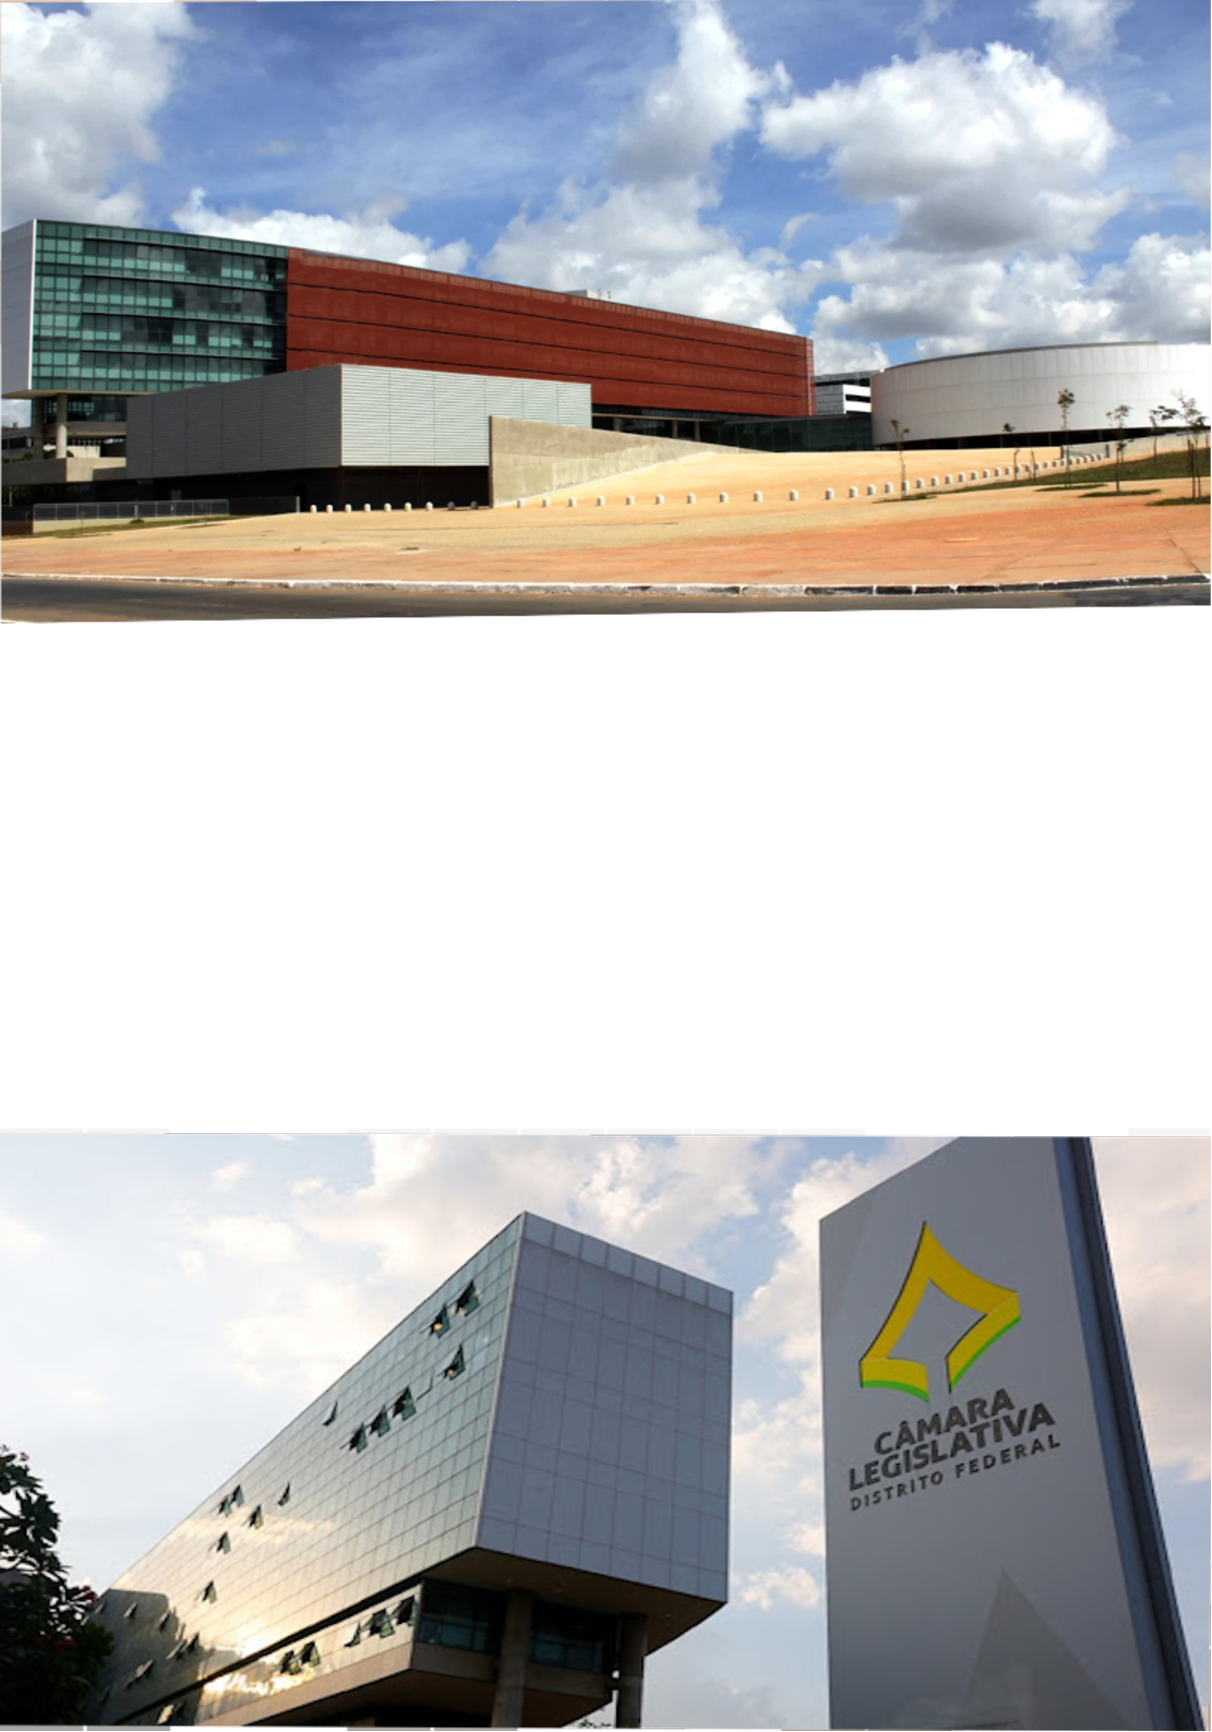
\includegraphics[width=\paperwidth]{capa.pdf}};
\draw (current page.center) node [fill=ocre!30!white,fill opacity=0.8,text opacity=1,inner sep=1cm]{\Huge\centering\bfseries\sffamily\parbox[c][][t]
{\paperwidth}
{
\centering \capatitulo\\[15pt] % Book title
{\Large \capasubtitulo}\\[20pt] % Subtitle
{\capaunidade} % Author name
}}; 
\end{tikzpicture}

\vfill

\endgroup
 % Capa
%
\includepdf[pages=-]{cfg/creditos.pdf}

% Esses debaixo nao vai ter mesmo
% nao descomentar
%% ####
% COPYRIGHT
% ####

\newpage
~\vfill
\thispagestyle{empty}

\noindent Copyright \copyright\ 2019 John Smith\\ % Copyright notice

\noindent \textsc{Published by Publisher}\\ % Publisher

\noindent \textsc{book-website.com}\\ % URL

\noindent Licensed under the Creative Commons Attribution-NonCommercial 3.0 Unported License (the ``License''). You may not use this file except in compliance with the License. You may obtain a copy of the License at \url{http://creativecommons.org/licenses/by-nc/3.0}. Unless required by applicable law or agreed to in writing, software distributed under the License is distributed on an \textsc{``as is'' basis, without warranties or conditions of any kind}, either express or implied. See the License for the specific language governing permissions and limitations under the License.\\ % License information, replace this with your own license (if any)

\noindent \textit{First printing, March 2019} % Printing/edition date
 % Copyright
%% ####
% APRESENTAÇÃO
% ####

\newpage
~\vfill
\thispagestyle{empty}

\noindent \textsc{Curso Técnico em Eletrotécnica, Instituto Federal Fluminense - Campus Itaperuna}\\

\noindent 
Caro estudante,

Bem-vindos à disciplina de Meio Ambiente e Energias Renováveis que tratará [...] para aprofundar seus conhecimentos sobre [...] no curso Técnico em Eletrotécnica do Instituto Federal Fluminense – Campus Itaperuna.

Para que seu estudo se torne proveitoso e prazeroso, esta disciplina foi organizada em [...] capítulos, com temas e subtemas que, por sua vez, são subdivididos em seções (tópicos), atendendo aos objetivos do processo de ensino-aprendizagem.
O capítulo 1, que trata [...], procuraremos compreender [...].  No capítulo 2, descreveremos
[...]. No capítulo 3, detalharemos [...]. Finalmente, no capítulo 4 refletiremos um pouco sobre [...]. Esperamos que, até o final da disciplina vocês possam:
- Ampliar a compreensão sobre [...];
- Conhecer [...];
- Identificar os aspectos [...];
- Compreender a importância [...];
Para tanto, a metodologia das aulas [...].

Porém, antes de iniciar a leitura, gostaríamos que vocês parassem um instante para refletir sobre algumas questões [...].
Não se preocupe.  Não queremos que vocês respondam de imediato todas essas questões.  Mas esperamos que, até o final, vocês tenham respostas e também formulem outras perguntas.

Vamos, então, iniciar nossas aulas? Bons estudos!

\vspace{3cm}
\DTMlangsetup{showdayofmonth=false}
\noindent \textit{1ª Ed., \today }
\DTMlangsetup{showdayofmonth=true}
 % Apresentação

%----
%	SUMÁRIO
%----

\usechapterimagefalse % If you don't want to include a chapter image, use this to toggle images off - it can be enabled later with \usechapterimagetrue


\addtocontents{toc}{\protect\hypertarget{TargetTableOfContents}{}}
\chapterimage{capitulos.pdf}
\pagestyle{empty}
\tableofcontents
\cleardoublepage
\pagestyle{fancy}

%----
%	DESENVOLVIMENTO
%----

%% ####
% DESENVOLVIMENTO
% ####

% Aqui você coloca os .tex na ordem que serão compilados
% Pode usar os comandos parte para dividir em partes se quiser

\part{PLANEJAMENTO}

\chapter{Afazeres}


\TODO{Aqui todos}


\section{Afazeres Gerais}

\TODO{Qualquer todo}





% \chapter{Dúvidas}


	\section{Dúvidas para Pedro}


\begin{enumerate}
	% \item Durante a Sprint de codificação, precisarão se reunir comigo?
	
	% \item Não estou vendo, no escopo, aonde vamos modelar as telas de cada Unidade do Sistema.
	
	
	% \item Quando seria importante fazer umas reuniões com o Gilberto para ver o sistema antigo?
	
	\item Final.
\end{enumerate}

	\section{Dúvidas para Fábrica/João}


\begin{enumerate}
	\item Nada
	
	% \item Vamos controlar apenas o protocolo ou vamos fazer o gerenciamento de distribuição dos artefato(s) que são criados? Fazer tudo.
	
	% \item Tem como armazenar os documentos word em uma tabela de banco de dados?
\end{enumerate}



	\section{Dúvidas Respondidas}

\subsection{Respostas para Wagner - Modelagem}

\begin{enumerate}
	
	\item A seta entre Avaliar OS e Histórico parece estar no sentido contrário. É feito um registro a cada avaliação ou é consultado o histórico para verificar se o trabalho já foi demandado?
	
	Sim, é consultado o histórico para verificar se o trabalho já foi demandado. Troquei o sentido da seta.
	
	
	\item O que acontece se o chefe da unidade não aprovar os artefatos?
	
	Se o chefe da unidade não aprovar os artefatos, ele devolve o artefato para o consultor legislativo corrigir.
	
	\item O demandante tem a opção de rejeitar a entrega?
	
	Não sei. Ver com eles.
	
	%\TODO[1]{Ver isso}	
	
	\item Acho que não precisa da seta entre Entregar Artefatos ao Solicitante e Solicitante já que o próximo passo é o envio do e-mail que é, para mim, o registro formal da entrega.
	
	Concordo.	
	
	\item Faltou o evento de início (círculo verde) e um evento de fim (círculo vermelho).
	
	O evento de início é o evento de início especial de recebimento de mensagem.
	
	O evento de final é o evento de final especial de envio de mensagem.	
	
	
	\item Pegar opinião entre modelo com retornos ou sem. 
	
	Vai ser com retornos.
\end{enumerate}

\subsection{Controle de Perfis e Papéis}


\begin{pergunta}[1]{Pergunta}
	Dúvida sobre algo que devo precisar no Sistema da ASSEL: 
	
	- Que informações sobre determinado usuário consigo pegar pelo Active Directory?
	
	- Tem como, pelo login, saber se o usuário é Consultor Legislativo ou Consultor Técnico Legislativo?
\end{pergunta}	

\begin{resposta}[1]{Resposta}
	não use o AD pra regra de negocio de sistema, pelo amor de deus!
\end{resposta}	

\begin{resposta}[1]{Resposta}
	Usar o AD então só para autenticação e depois fazer um controle de papéis interno dentro do sistema. Provavelmente vou precisar de ajuda de vcs quando eu chegar nessa etapa.
	
	Lá na ASSEL, dependendo do Cargo da Pessoa, unidade, lotação, etc, cada um só terá acesso a uma determinada "tela" .
\end{resposta}	

\begin{resposta}[1]{Resposta}
	Acho arriscado amarrar as atribuições em função do cargo. Com as mudanças nas chefias e no quadro de servidores, podem mudar do dia para a noite. No PLe, as funcionalidades são utilizadas para configurar os perfis de acesso e alterações podem ser feitas a qualquer tempo por um administrador do sistema.
\end{resposta}	

\begin{resposta}[1]{Resposta}
	a falar isso: esquece a ideia de "cargo", pensa em "perfil". é atribuição do usuario gestor determinar qual pessoa tem qual perfil em qual unidade. Se ela qusier colcoar um faxineiro com perfil de CL, é problema dele, nao nosso.
	
	e uma mesma pessoa pode ter varios papeis. um chefe pode ser tambem um CL. E tambem assessor de um deputado.
\end{resposta}	


\chapter{Diário}

\section{26 Nov 2023}

Criei esse ambiente latex a partir de al para escrever alguma documentação.


%\part{MODELAGEM}

%\chapter{Entrevistas}

\section{Gilberto - Apoio da ASSEL}

O sistema deve ser integrado ao SEI de forma a documentar no SEI o histórico na mudança dos estados.

Então, as Ordens de Serviços para a Assel, que atualmente vem por intermédio de um Formulário do SEI, deveriam vir por intermédio de um Formulário Preenchido dentro do Portal, que alimenta o sistema e, por sua vez, o sistema registra isso no SEI.

\begin{requisito}{Requisito}
	Deve haver alguma forma de registrar quem foi o(s) solicitante(s) de uma Demanda. Inclusive, se combinado, quando o Solicitante entrar no sistema para fazer uma nova Solicitação, ele consiga ver o histórico dos pedidos que ele fez acompanhado do Status dos pedidos já realizados por ele: Em Execução, Concluído, Suspenso, etc… Isso seria possível através de uma ``Tela de Acompanhamento'' na qual o Solicitante loga-se e pode acompanhar o ``Estado'' de cada uma de suas demandas. Isso atende A1-3:19.
\end{requisito}

\subsection{A1 8:20 até 16:00 - Duas ou mais demandas de mesmo PL}

	\textbf{Questão de ter duas ou mais Demandas relacionadas a um mesmo projeto, mas designado por Deputados diferentes, e portanto, de Comissões diferentes.} 
  
	Nesses casos, os pareceres serão diferentes, então mesmo que as duas demandas estejam relacionadas com um mesmo Projeto de Lei, os pareceres terão de ser feitos com pontos de vista diferentes e, assim, serão pareces diferentes. No processo de “RECEBER OS E APOIAR” o pessoal do Apoio quer ser capaz de verificar no histórico, todos os processos relacionados a, por exemplo, uma mesma PL. Assim, mesmo que seja uma demanda nova “que necessite elaboração” , ela já pode encaminhar essa informação para o Consultor que fará o trabalho. Então o processo de “APOIO” gera artefatos novos que serão apensados à OS. Um desses artefatos são informações de, por exemplo, demandas já realizadas pela ASSEL que relacionam-se com aquela demanda. Esse “pacote”  é que segue para frente.

	Em relação a isso, vislumbro uma tela onde o Apoio tem como se fosse uma “Caixa de Entrada” com as demandas recebidas, por quem, etc… Ali, o servidor da ASSEL será capaz de analisar cada demanda recebida e destiná-la. Quando o destino for “Necessita de Elaboração” ele já pode anexar no “Processo” informações de outras demandas já concluídas pela ASSEL que estão relacionadas àquela demanda. O sistema já poderia até sugerir isso para ele automaticamente.  

\subsection{A1 17:00 - Código de Nomenclatura}

	Ele fala de uma metodologia que eles já usam atualmente para nomear o artefato que será produzido. É como se fosse uma Primary Key, isto é, um Código Chave, um identificador único que eles criam para cada documento que será elaborado de forma que isto facilite, depois, o controle deles. Acho importante mantermos essa forma de organizar as coisas, ou se não, podemos melhorar, mas com o cuidado de “melhorar mas manter compatibilidade”.

\subsection{A1 18:30 - Diversos Tipos de Demandas}

Não podemos restringir o sistema a “Demandas relacionadas somente com PLs”. O sistema deve ser capaz de controlar atividades relacionadas a quaisquer tipo de “Demandas” dentre os tipos de Demandas Possíveis.

\subsection{A1 20:55}

Está falando os diferentes tratamentos dados aos diferentes “tipos de demandas”. Cada “Demanda” tem um “Tipo” e “Demandas” de cada “Tipo” terão atributos diferentes. Alguns desses atributos já virão preenchidos.

Aqui no *1 deve haver uma etapa na qual o Apoio consegue classificar e até “corrigir” a Demanda que chegou. Talvez na “Tela de Envio” o usuário poderá selecionar o tipo de demanda que ele “Acha” que é e já preencher os dados.

E haverá uma “tela de classificação” na qual o Servidor do Apoio poderá ver os dados brutos preenchidos pelo Solicitante e classificar aquela demanda corrigindo se isso for necessário. 


\begin{exemplo}{Exemplo}
	O Solicitante solicita uma Consulta e em um campo “Descrição” ele descreve o que quer. Chegando na ASSEL, o Servidor do Apoio analisa o pedido e verifica que o que o Solicitante deseja é, na verdade, ´um “Estudo” e não uma “Consulta”. Reclassifica essa demanda e segue.
\end{exemplo}

\begin{requisito}{Requisito}
	Pesquisa textual dentro de todos os Documentos já produzidos pela ASSEL.
\end{requisito}

\begin{exemplo}{Exemplo}
	APOIO = RECEBER $\rightarrow$ FILTRAR $\rightarrow$ REGISTRAR NO SISTEMA $\rightarrow$ ENVIA PARA CHEFE DISTRIBUIR
\end{exemplo}

Aqui um dos Metadados possíveis seria a possibilidade do Apoio “Sugerir” para qual unidade isso deve ser distribuído. Depois, a Chefe, no momento de Distribuir para a Unidade, recebe essa sugestão e decide se “Acata e Aprova” ou se manda para outra Unidade.

Haverá uma “Tela de Distribuição” na qual somente o Chefe pode assessar e lá o Chefe deve distribuir o processo ou mandar voltar.

Acho que sempre deve existir o botão de “VOLTAR” ou “RETORNAR” com uma mensagem de forma que correções de fluxo possam ser realizados. Por exemplo, alguem erra e manda pra frente. Lá na frente, a pessoa pode mandar “VOLTAR” e claro, justifica. Ou seja, depois que vai, pra voltar, quem manda de volta é quem recebe.

\begin{requisito}{Requisito}
	Toda a ASSEL terá que ter acesso ao Sistema. O Sistema é quem distribui  etc.
\end{requisito}


13/05/21 Gilberto me disse:

\begin{importante}[1]{Ao receber OS}
	Verificando a Modelagem de processo, na questão de recebimento da Ordem de Serviço, ocorre que em primeiro momento quem recebe a demanda no Apoio é a própria Chefe da Assessoria que lê e defini qual a Unidade da Assessoria Legislativa é competente para analisar o pedido, depois distribui para nós alimentarmos os sistema atual, nessa etapa verificamos se já houve algum pedido do mesmo solicitante, ou de outro. A OS estando OK para seguir, liberamos o documento para seguir, geramos o Despacho para a Chefe da Assessoria Legislativa assinar e dar seguimento.
\end{importante}

Assim, já entendi que a Chefe da Assel deve fazer as interfaces com os demais atores.

O Apoio conversa unicamente com a Chefe da Assel.  

 


\section{Ana - Consultora Legislativa da UDA}

A Ana é Consultora Legislativa da UDA.

\subsection{Papéis Desempenhados}

Ela me alertou que o CL pode trabalhar de duas formas:

\begin{enumerate}
	\item Titular da Demanda: Responsável pelo trabalho de elaboração dos Artefato(s) demandados.
	
	\item Revisor de Artefato(s): Responsável pelo trabalho de revisar o trabalho de outro colega.
\end{enumerate}

Inclusive ela me disse que esse papel de ``Revisão'' faz parte formal do trabalho do CL.

\begin{requisito}{Requisito}
	Portanto, é importante separar esse Estado onde o processo se encontra. Está sendo elaborado ou está sendo revisado?
\end{requisito}

\subsection{Função do Chefe}

Quando os trabalhos de elaboração e revisão terminam, os artefato(s) são entregues para o Chefe, que faz uma revisão ``menor'' nos produtos.

Basicamente eles apenas tomam conhecimentos e devolvem os artefatos para o Apoio.

\subsection{Controle de Estado de Elaboração}


\begin{requisito}{Requisito}
	Haver forma de ``medir'' ou se fazer controle de estado da Elaboração / Revisão;	
\end{requisito}


\subsection{Distribuição dos Artefatos}

Os artefato(s) criados vão para a Pasta do CL. O apoio tem acesso a todas as pastas de todos os CLs.

Os CLs só tem acesso às suas próprias pastas na rede.

Por enquanto, a troca de arquivos ocorre dessa forma. Pastas na rede.


\section{Josué Alves - Chefe da USE}

Josué Alves é Chefe da USE

\subsection{01m30 - Aspectos Internos}

Fala das minutas de parecer pela prejudicialidade.

\subsection{02m30 - Elaboração e Distribuição}

``Atividade de Elaboração'' pode ser realizada pelo Próprio Chefe de Unidade desde que ele seja Consultor Legislativo. Caso, ele seja CTL, então ele não pode.

\begin{importante}{Puxar Demanda}
	Na atividade de ``Distrubuição de OS'' do Chefe da Unidade, em vez do ``Chefe Empurrar'' a demanda para o CL. Há opção do CL escolher a atividade para sí, ie, puxar.			
\end{importante}


\subsection{04m40 - Sigilo da Minuta de Parecer}

05m20 - Minuta de Pareces, Nota Técnica, Estudo (tudo eu acho) são atividades cujo conteúdo durante a elaboração são sigilosos.

\subsection{07m25 - Questão do controle de estado da Demanda}

\begin{funcionalidade}[1]{Possibilidade de o Solicitante poder acompanhar aonde o trabalho está}
	Possibilidade de o Solicitante poder acompanhar aonde o ``trabalho está''.
\end{funcionalidade}

Exemplo: Está em elaboração, está em revisão, está no apoio, está esperando distribuição, etc...

\subsection{09m12 - Funcionalidade: Vínculo entre Demanda e PL}

Acompanhar estado da Proposição que originou o Parecer.

\begin{funcionalidade}{Acompanhar estado da Proposição que originou o Parecer}
	Se houver vínculo entre a demanda do tipo ``Minuta de Parecer'' com o PL originário em tramitação, então seria importante que o sistema oferecesse uma forma de verificar o estado do PL.
	
	Aqui talvez seja necessário fazer integração com o Sistema do PLE.
\end{funcionalidade}

\subsection{14m10 - Aula sobre Proposição}

PELO
PLC
PL
PDC
PR
Emendas

\subsection{16m30 - Nomenclatura da OS}

Nomenclatura: OS ou Solicitação

\subsection{19m16 - Classificação das Demandas}

\begin{funcionalidade}{Classificação das Demandas}
	Dentro do processo das Unidades, cada unidade deveria poder classificar suas demandas da forma que quisesse.
	
	É quase igual ao sei onde podemos criar marcadores e depois filtrar por marcadores com diferentes cores e etc.		
\end{funcionalidade}	

Na unidade do Josué eles classificam as demandas.

 
\subsection{22m30 - Distribuição interna das demandas}

Possibilidade de puxar as demandas para sí mais do que esperar o Chefe atribuir para vc uma demanda.

Normalmente o \CL ele próprio escolhe o trabalho que vai realizar.

Claro, se sobra algo lá que ninguem quer, cabe ao Chefe designar alguém para desenvolver determinada demanda.

\subsection{25m00 - Como as revisões são escolhidas e verificação}

Nome: Revisão e Verificação.

Nome: Verificação;

Nome: Revisão Final;

\subsection{29m50 - Outros documentos}

Aqui eu aviso que o sistema não pode substituir o SEI. Então, vocês continuarão usando o SEI para coisas paralelas.

Agora, as solicitações e o processo, embora será, de alguma forma documentada no SEI, vocês usaram o sistema pois aí o sistema trará mais recursos. 

Josué diz que podem ser necessários fazer consultas aos orgaos sobre os pareces. Seria bom que essas consultas fossem relacionadas com a demanda.

Talvez seria interessante conversar mais sobre essa questão.

\begin{importante}{Automatiza o SEI?}
 Automatizar o SEI para fazer consultas relacionadas a demandas em andamento?	
 
 Lógico que não.
 
 Esse caso deve ser sim conversado e aprofundado. Mas no futuro. Vamos trabalhar no MVP por enquanto. 
\end{importante}

\section{Milena - Chefe da Assel}

A ``Distribuição'' é do tipo empurra. Ela e o apoio analisam a OS e mandam para o Unidade que eles acham que é.

Ela atenta para a questão do Sigilo ao mesmo tempo que deve haver possibilidade do CL pesquisar o Banco de Dados. 

\begin{importante}{Pesquisar sem comprometer Sigilo}
	Deverão haver mais conversar para entender como seriam feitas essas pesquisas sem comprometer o Sigilo.
	
	Quem pode pesquisar? Etc...	
\end{importante}

Milena também pontua que o Sistema deve eliminar a necessidade de realizar o Acesso Remoto nos computadores. O sistema deve funcionar on-line na Internet mediante autenticação do usuário (login). 

Seria bom que o sistema também fosse responsável para receber os artefato(s) e realizar a distribuição desses artefato(s) em cada fase até finalizar entregando isso para o Solicitante.

Ela diz que um problema que eles tem é que as vezes eles não conseguem acessar a pasta deles na rede e isso impacta o trabalho.


\section{Jeison - Chefe da UCJ}

\subsection{Nota Técnica}

Ao ``Elaborar Artefatos'' pode surgir a necessidade de criar uma ``Nota Técnica'' com algo que deve ser informado ao Solicitante.

\begin{importante}{Nota Técnica}
	Questão da Nota Técnica: A demanda pode gerar a necessidade de que o \CL crie uma Nota Técnica contendo conteúdo importante.
	
	O ideal é fazer novas conversas sobre isso.		
\end{importante}

\subsection{Pesquisa Prévia no Apoio}

Incluir na atividade de apoio a capacidade de que, quando entende-se que necessita-se de elaboração, essa elaboração possa ser precedida de uma pesquisa prévia. 

Ou seja, ao processo já podem ser inseridos artefato(s) de auxílio aos Consultores Legislativos que receberão a demanda lá na frente no futuro.

   
\section{Cláudio UEF}


% Isso já foi contemplado.
%\begin{importante}[1]{Importante}
%	Não é obrigatório passar pela revisão;
%\end{importante}



Ele traz outras funcionalidades:

- Acompanhamento Temporal


\begin{importante}{Mudança de relator de um OS}
	Mudança de relator de um OS.
\end{importante}

%\TODO{Incluir Ciencia na ASSEL antes de Arquivar}

\begin{importante}{Abortar a OS}
	Possibilidade de abortar a OS a qualquer momento.	
\end{importante}

Mudar nome do losango de ``Necessita de Elaboração'' para ``Cumpre Requisitos?''


\section{Ana Alice UDA}


\begin{funcionalidade}{Organização via bloco interno}
	Quando for a época a gente vê isso. Ana disse que podia mostrar.
\end{funcionalidade}


Seria bom pedir para ela me mostrar se possivel no SEI como é a atual organização via Bloco Interno das coisas no SEI.

Nessa parte eu pensei que o ideal seria criar um sistema de organização igual às Tags do Gmail. 

%\TODO{Ver com a Ana Alice se um sistema de Tags... }

%Ver com a Ana Alice se um sistema de Tags igual ao do Gmail satisfaria as necessidades dela de organização.

%Vou fazer assim


\section{Pedro da Basis}

Para o Módulo II fazer Exportação de Dados para BI.
	
	






































\chapter{Informações Coletadas}

%Depois de consolidado cada seção aqui tem que virar uma nota técnica no SEI.

\section{Unidades Internas}

\begin{itemize}
	\item ASSEL - Assessoria Legislativa;
	\item UCJ - Unidade de Constituição e Justiça;
	\item URP - Unidade de Redação Parlamentar e Consolidação dos Textos Legislativos;
	\item UEF - Unidade de Economia e Finanças;
	\item USE - Unidade de Saúde, Educação, Cultura e Desenvolvimento Científico e Tecnológico; 
	\item UDA - Unidade de Desenvolvimento Urbano e Rural e Meio Ambiente;
\end{itemize}


\section{Unidades Externas}

São quaisquer unidades do SEI que forem cadastradas no sistema e atuam somente como Solicitantes.


\section{Tipos de Solicitações}

%\TODO{Consolidar e subir para SEI como Nota Técnica}

As demandas recebidas pela ASSEL classificam-se no \textbf{Tipos de Solicitação} a seguir:

%Isto foi me enviado pelo Gilberto no dia 27/04/21.

\begin{itemize}
	\item Consulta (CONS)
	\item Estudo (EST)
	\item Minuta de Pronunciamento / Discurso (PRO)
	\item Minuta de Parecer
	\begin{itemize}
		\item Denúncia (DEN)
		\item Indicação (IND)
		\item Mensagem (MENS) 
		\item Projeto de Decreto Legislativo (PDL)
		\item Proposta de Emenda à Lei Orgânica (PELO)
		\item Projeto de Lei (PL)
		\item Projeto de Lei Complementar (PLC) 
		\item Projeto de Resolução (PR)
		\item Moção (MOC)
		\item Recurso (REC)
		\item Requerimento (RQ)		
    \end{itemize}


	\item Minuta de Proposição (MP)
	\begin{itemize}
		\item Denúncia (DEN)
		\item Indicação (IND)
		\item Mensagem (MENS) 
		\item Projeto de Decreto Legislativo (PDL)
		\item Proposta de Emenda à Lei Orgânica (PELO)
		\item Projeto de Lei (PL)
		\item Projeto de Lei Complementar (PLC) 
		\item Projeto de Resolução (PR)
		\item Moção (MOC)
		\item Recurso (REC)
		\item Requerimento (RQ)		
    \end{itemize}

	\item Nota Técnica (NT)
	\item Relatório de Veto (RV)
	\item Outros (OUT)
\end{itemize}

\begin{importante}{Mudar aqui muda lá}
	Mudar esses tipos tem que definir novos códigos em \ref{ref:codigos}.
\end{importante}

\section{Módulos}

	Verificamos dois principais necessidades da \ASSEL:
	
	\begin{itemize}
		\item  \textbf{Sistema de Protocolo} - 	A necessidade da \ASSEL \xspace é de um sistema de protocolo integrado ao SEI que controle as atividades da unidade.  
		
		\item \textbf{Controle e Distribuição dos Artefato(s)} - Necessidade de controlar a forma como os artefato(s) desenvolvidos são distribuidos para os seus solicitantes.
	\end{itemize}

	Assim, acredita-se que para fins de desenvolvimento o sistema pode ser desenvolvidos em dois módulos.

\subsection{Módulo I - Sistema de Protocolo}

	Num primeiro momento seria desenvolvido um \textbf{sistema de protocolo integrado ao SEI} para controlar o fluxo de atividades da \ASSEL.
	
	Neste primeiro momento, a \textbf{forma de distribuição} dos artefato(s) criados pela \ASSEL não seria objeto de desenvolvimento. Isto é, a \ASSEL continuaria fazendo o controle e distribuição de Artefato(s) da maneira antiga, isto é, manualmente, utilizando a estrutura de rede da casa.   


\subsection{Módulo II - Controle e Distribuição de Artefato(s) produzidos}

	Em um segundo momento, após ter uma versão do Módulo I desenvolvida, em produção, funcionando com recursos mínimos, passaríamos a focar em fazer o \textbf{Controle e Distribuição de Artefato(s) produzidos}.
	
	Assim, neste momento, a distribuição dos artefato(s) produzidos deixariam de ser uma tarefa manual executada pela equipe de Apoio da \ASSEL e passaria a ser executada pelo próprio sistema.
	
	Em um experimento de imaginação, quando o \CL finalizasse uma demanda, ele faria \emph{upload} do(s) arquivos produzidos para o sistema e na outra ponta, o Solicitante faria o \emph{download} desses arquivos.
	
	Neste momento, as preocupações com os requisitos não funcionais de ``Sigilo'' passariam a ser considerados. 	


\section{Requisitos Funcionais}


\subsection{Requisito: Capacidades de Pesquisa}

Trata-se da capacidade de realizar pesquisas como:

\begin{itemize}
	\item Pesquisa textual dentro de todos os documentos já produzidos pela \ASSEL.
	
	\item Pesquisar os metadados de processos já tramitados pela Assel e que originaram artefato(s).	
\end{itemize}

\subsection{Requisito: Monitorar Estado das Solicitações}

Capacidade de permitir que o solicitante saiba onde o processo está e receba informações sobre o estado da solicitação.

\section{Requisitos Não Funcionais}

\subsection{ReqNFunc: Integração com o SEI}

Uma das restrições do projeto previsto no TAP é que o Sistema não pode substituir o SEI. Então um requisito não funcional muito importante é que o Sistema funcione juntamente com o SEI.


\subsection{ReqNFunc: Sigilo}

Da elaboração até a entrega dos artefato(s) aos Solicitantes, esses artefato(s) são sigilosos. Ou seja, só ganhará acesso ao artefato quem demandou.

\subsection{ReqNFunc: Acesso via Internet}

	O Sistema deve eliminar a necessidade de realizar o Acesso Remoto nos computadores. O sistema deve funcionar on-line na Internet mediante autenticação do usuário (login).



%\chapter{Modelagem do Macroprocesso}

	\section{Raia: Apoio da Assessoria Legislativa}

		\subsection{Ativ: Receber Ordem de Serviço}
		
		\subsection{Ativ: Avaliar OS}
				
		\subsection{Ativ: Notificar Solicitante}
		
		\subsection{Ativ: Entregar Artefatos ao Solicitante}		
		
		\subsection{Ativ: Catalogar e Arquivar Artefatos}		


	\section{Raia:Chefe Assessoria Legislativa}

		\subsection{Ativ: Distribuir OS para Unidade}		


	\section{Raia:Chefe da Unidade}

		\subsection{Ativ: Distribuir OS para Consultor Legislativo}		
		
		\subsection{Ativ: Aprovar Artefato(s)}		
		

	\section{Raia: Consultor Legislativo}

		\subsection{Ativ: Elaborar Artefato(s)}


%\chapter{Estudo}

Nesse capítulo pretendo começar a escrever o documento final que vai para o SEI contendo a modelagem do processo, explicações, requisitos, enfim, será um documento de partida para entregar para a Fábrica de Software.


\section{Introdução}

Introduzir o projeto do sistema.

\subsection{Assessoria Legislativa}

Falar da Assel

\subsubsection{Estrutura}

\subsubsection{Atores}

\subsection{Necessidades e Módulos}

Falar das necessidades e Módulos


\section{Modelagem de Processos}

Aqui vai a modelagem em sí explicadinha.





\chapter{Codificação para as Solicitações}
\label{ref:codigos}

\section{Definição}

As ``Ordens de Serviço'' ou ``Solicitações'' que transitam pelo Sistema ASSEL terão um código ``humano'' associado a ele. Esse código deve ser \textbf{único} de modo que só exista um único código associado a cada OS. Este campo é uma forma de dar nomes únicos a cada Solicitação de forma que seja fácil se referir e localizar uma Solicitação dentre todas as existentes.


\begin{nota}[1]{Nota: Esse código não deve ser usado como Chave Primária}
	Não é interessante, internamente no banco de dados, utilizar esse código como chave primária pois em alguns casos pode ser necessário modificar o código inicial atribuído a uma OS. 	
	
	O caso que isso aconteceria seria quando uma Solicitação fosse revisada e seus atributos de tipo e/ou subtipo tivessem de mudar. Nesse caso, o código deverá ser alterado junto, respeitando o critério de unicidade.
\end{nota}


Os códigos terão regra de formação de acordo com os Tipos e Subtipos das OSs.

\section{Regra de Formação Grupo I}

\subsection{Aplicação - Grupo I}

\begin{env-aplica}{Regra de Formação Grupo I são aplicadas a Solicitações dos Tipos:}
	\item Consulta (CONS)
	\item Estudo (EST)
	\item Minuta de Pronunciamento / Discurso (MPRON)
	\item Nota Técnica (NT)
	\item Relatório de Veto (RV)
	\item Outros (OUT)	
\end{env-aplica}

\subsection{Regra - Grupo I}

\begin{env-regra}{Regra de formação Grupo I}
	``SIGLA-TIPO'' + ``NÚMERO'' + ``-'' + ``ANO''
\end{env-regra}

\textbf{Aonde}:
\begin{itemize}
	\item \textbf{SIGLA-TIPO}: Sigla referente ao tipo conforme tabela. Ex.: CONS, EST, MPRON, NT, RV, OUT.
	\item \textbf{NÚMERO}: Contador relativo ao tipo e ano. Máscara de 3 dígitos preenchidos com 0. Ex.: 001, 010, 100. Se maior que 3 dígitos, usar o número todo.
	\item \textbf{ANO}: Ano da Solicitação com 4 dígitos. Ex.: 2021.
\end{itemize}

\subsection{Siglas - Grupo I}

\begin{table}[!h]
	\begin{center}
		\begin{tabular}{|p{0.4\textwidth}|c|c|}
			\hline
			\rowcolor{lightgray!50} \multicolumn{3}{|c|}{\Large Siglas e Exemplos - Grupo I \normalsize} \\ \hline \hline
			% CABEÇALHO        
			\rowcolor{lightgray}\textbf{Tipo} & \textbf{Sigla} & \textbf{Exemplo} \\ \hline
			% CONTEÚDO
			% Código escrito manualmente
			\rowcolor{corCOULD!10} \textbf{Cons}ulta (oria) & \textbf{CONS} & CONS002-2021  \\ \hline
			\rowcolor{corCOULD!20} \textbf{Est}udo & \textbf{EST} & EST080-2021 \\ \hline
			\rowcolor{corCOULD!10} \textbf{M}inuta de \textbf{Pron}unciamento / Discurso & \textbf{MPRON} & MPRON120-2021 \\ \hline
			\rowcolor{corCOULD!20} \textbf{N}ota \textbf{T}écnica  & \textbf{NT} & NT010-2021 \\ \hline
			\rowcolor{corCOULD!10} \textbf{R}elatório de \textbf{V}eto  & \textbf{RV} & RV010-2021 \\ \hline
			\rowcolor{corCOULD!20} \textbf{Out}ros & \textbf{OUT} & OUT100-2021 \\ \hline
		\end{tabular}    
		\caption{\label{tab:cod:grupoi} Codificação Grupo I.}
	\end{center}
\end{table}

\subsection{Exemplos - Grupo I}

\begin{itemize}
	\item \textbf{Exemplo 1 - Estudo}:
	
	\begin{enumerate}
		\item Suponha que o Solicitante peça uma nova OS do tipo ``Estudo'' e ano atual seja o ano de 2021.
		
		\item O sistema verifica que no ano de 2021 já existem 4 (quatro) ``Estudos'' cadastrados no sistema. Portanto, o número dessa nova OS será 4 + 1 = 5 com máscara NNN.
		
		\item Então o código desta nova solicitação será formado por ``EST'' + ``005'' + ``-'' + ``2021'' formando \textbf{EST005-2021}.			
	\end{enumerate}

	\item \textbf{Exemplo 2 - Consulta}:

\begin{enumerate}
	\item Suponha que o Solicitante peça uma nova OS do tipo ``Consulta'' e ano atual seja o ano de 2022.
	
	\item O sistema verifica que no ano de 2022 ainda não foram realizados Solicitações do tipo ``Consulta'' no sistema. Portanto, o número dessa nova OS será 0 + 1 = 1 com máscara NNN. 
	
	\item Então o código desta nova solicitação será formado por ``CONS'' + ``001'' + ``-'' + ``2022'' formando \textbf{CONS001-2022}.			
\end{enumerate}

	\item \textbf{Exemplo 3 - Outro}:

\begin{enumerate}
	\item Suponha que o Solicitante peça uma nova OS do tipo ``Outro'' e ano atual seja o ano de 2021.
	
	\item O sistema verifica que no ano de 2021 já existem 999 OSs do Tipo ``Outro'' cadastrados no sistema. Portanto, o número dessa nova OS será 999 + 1 = 1000.
	
	\item Então o código desta nova solicitação será formado por ``OUT'' + ``1000'' + ``-'' + ``2021'' formando \textbf{OUT1000-2021}.			
\end{enumerate}

\end{itemize}

\section{Regra de Formação Grupo II - Minuta de Proposição (MP)}

\subsection{Aplicação - Grupo II}

\begin{env-aplica}{Aplica-se a Solicitações do Tipo ``Minuta de Proposição (MP)'' com os seguintes subtipos:}
	\item Denúncia (DEN)
	\item Indicação (IND)
	\item Mensagem (MENS) 
	\item Projeto de Decreto Legislativo (PDL)
	\item Proposta de Emenda à Lei Orgânica (PELO)
	\item Projeto de Lei (PL)
	\item Projeto de Lei Complementar (PLC) 
	\item Projeto de Resolução (PR)
	\item Moção (MOC)
	\item Recurso (REC)
	\item Requerimento (RQ)		
\end{env-aplica}

\subsection{Regra - Grupo II}

\begin{env-regra}{Regra de formação Grupo II - Minuta de Proposição (MP)}
	``MP'' + ``NÚMERO'' + ``SIGLA-SUBTIPO'' + ``ANO''
\end{env-regra}
 
\textbf{Aonde}:

\begin{itemize}
	\item \textbf{MP}: Texto fixo MP. 
	\item \textbf{NÚMERO}: Contador relativo ao tipo de Minuta de Proposição do subtipo escolhido e ano. Máscara de 3 dígitos preenchidos com 0. Ex.: 001, 010, 100. Caso o número ultrapasse 999 o número deve ser escrito com todos os dígitos necessários. 

	\item \textbf{SIGLA-SUBTIPO}: Sigla referente ao subtipo conforme tabela. Exs.: PL, PELO, etc.

	\item \textbf{ANO}: Ano da Solicitação com 4 dígitos. Ex.: 2021.
\end{itemize}

\subsection{Siglas - Grupo II}

\begin{table}[!h]
	\begin{center}
		\begin{tabular}{|p{0.4\textwidth}|c|c|}
			\hline
			\rowcolor{lightgray!50} \multicolumn{3}{|c|}{\Large Siglas Grupo II - Minutas de Proposição (MP) \normalsize} \\ \hline \hline
			% CABEÇALHO        
			\rowcolor{lightgray}\textbf{Subtipo} & \textbf{Sigla} & \textbf{Exemplo} \\ \hline
			% CONTEÚDO
			% Código escrito manualmente
			\rowcolor{corCOULD!10} \textbf{Den}úncia & \textbf{DEN} & MP001DEN-2021 \\ \hline
			\rowcolor{corCOULD!20} \textbf{Ind}icação & \textbf{IND} & MP020IND-2020 \\ \hline
			\rowcolor{corCOULD!10} \textbf{Mens}sagem & \textbf{MENS} & MP220MENS-2020 \\ \hline
			\rowcolor{corCOULD!20} \textbf{P}rojeto de \textbf{D}ecreto \textbf{L}egislativo & \textbf{PDL} & MP010PDL-2021 \\ \hline
			\rowcolor{corCOULD!10} \textbf{P}roposta de \textbf{E}menda à \textbf{L}ei \textbf{O}rgânica & \textbf{PELO} & MP002PELO-2021 \\ \hline
			\rowcolor{corCOULD!20} \textbf{P}rojeto de \textbf{L}ei & \textbf{PL} & MP001PL-2022 \\ \hline
			\rowcolor{corCOULD!10} \textbf{P}rojeto de \textbf{L}ei \textbf{C}omplementar & \textbf{PLC} & MP001PLC-2022 \\ \hline
			\rowcolor{corCOULD!20} \textbf{P}rojeto de \textbf{R}esolução & \textbf{PR} & MP010PR-2022 \\ \hline
			\rowcolor{corCOULD!10} \textbf{Moc}ão (Moção) & \textbf{MOC} & MP010MOC-2022 \\ \hline
			\rowcolor{corCOULD!20} \textbf{R}e\textbf{c}urso & \textbf{RC} & MP001RC-2021 \\ \hline			
			\rowcolor{corCOULD!10} \textbf{R}e\textbf{q}uerimento & \textbf{RQ} & MP001RQ-2021 \\ \hline
		\end{tabular}    
		\caption{\label{tab:cod:grupoii} Codificação Grupo II.}
	\end{center}
\end{table}

\subsection{Exemplos - Grupo II}

\begin{itemize}
	\item \textbf{Exemplo - MP do tipo PDL}:
	
	\begin{enumerate}
	\item Suponha que o Solicitante peça uma nova OS do tipo ``Minuta de Proposição'' do subtipo ``Projeto de Decreto Legislativo''  e ano atual seja o ano de 2021.
	
	\item O sistema verifica que no ano de 2021 já existem 19 minutas de proposição do subtipo ``Projeto de Decreto Legislativo'' cadastrados no sistema. Portanto, o número dessa nova OS será 19 + 1 = 20 com máscara NNN.
	
	\item Então o código desta nova solicitação será formado por ``MP'' + ``020'' + ``PDL'' + ``-'' + ``2021'' formando \textbf{MP020PDL-2021}.			
	\end{enumerate}

\end{itemize}


\section{Regra de Formação Grupo III - Minutas de Parecer}

As solicitações do tipo ``Minuta de Parecer'' correspondem ao maior percentual de solicitações. Além disso, toda minuta de parecer está associada a uma Proposição e a uma Comissão.

Dessa forma, a regra de formação para solicitações do tipo ``Minuta de Parecer'' é especial.  

Ela começa com a sigla do subtipo, informa o número e ano da proposição, uma letra para especificar a Comissão e um número sequencial.  

\subsection{Aplicação - Grupo III}

\begin{env-aplica}{Aplica-se a Solicitações do Tipo ``Minuta de Parecer'' com os seguintes subtipos:}
	\item Denúncia (DEN)
	\item Indicação (IND)
	\item Mensagem (MENS) 
	\item Projeto de Decreto Legislativo (PDL)
	\item Proposta de Emenda à Lei Orgânica (PELO)
	\item Projeto de Lei (PL)
	\item Projeto de Lei Complementar (PLC) 
	\item Projeto de Resolução (PR)
	\item Moção (MOC)
	\item Recurso (REC)
	\item Requerimento (RQ)		
\end{env-aplica}

\subsection{Regra - Grupo III}

\begin{env-regra}{Regra de formação Grupo III - Minuta de Parecer}
	``SIGLA-SUBTIPO'' + ``NÚMERO DA PROPOSIÇÃO'' + ``LETRA DA COMISSÃO'' + ``NÚMERO SEQUENCIAL'' + ``-''  + ``ANO DA PROPOSIÇÃO''.
\end{env-regra}

\textbf{Aonde}:

\begin{itemize}
	\item \textbf{SIGLA-SUBTIPO}: Sigla referente ao subtipo conforme tabela. Exs.: PL, PELO, etc.


	\item \textbf{NÚMERO DA PROPOSIÇÃO}: Número da proposição associada com máscara NNN. Caso o número de dígitos da proposição seja maior do que 3, usar o número com todos os dígitos.
	
	\item \textbf{LETRA DA COMISSÃO}: Cada Comissão tem uma letra associada conforme tabela. 
	
	\item \textbf{NÚMERO SEQUENCIAL}: Contador relativo ao tipo de Minuta de Parecer do subtipo escolhido, Comissão e Ano. Sem máscara. Caso o número ultrapasse 9 o número deve ser escrito com todos os dígitos necessários. 	
	
	\item \textbf{ANO DA PROPOSIÇÃO}: Ano da \emph{Proposição} com 4 dígitos. Ex.: 2021.
\end{itemize}

\subsection{Letras das Comissões - Grupo III}

Ver tabela \ref{tab:cod:grupoiiil}.

\begin{table}[b]
	\begin{center}
		\begin{tabular}{|p{0.8\textwidth}|c|}
			\hline
			\rowcolor{lightgray!50} \multicolumn{2}{|c|}{\Large Letras Comissões para Grupo III - Minutas de Parecer \normalsize} \\ \hline \hline
			% CABEÇALHO        
			\rowcolor{lightgray}\textbf{Comissão} & \textbf{Letra} \\ \hline
			% CONTEÚDO
			% Código escrito manualmente
			\rowcolor{corCOULD!10} CCJ - Comissão de Constituição e Justiça & \textbf{J} \\ \hline			
			\rowcolor{corCOULD!20} CEOF - Comissão de Economia Orçamento e Finanças & \textbf{F} \\ \hline			 
			\rowcolor{corCOULD!10} CAS - Comissão de Assuntos Sociais & \textbf{S} \\ \hline			
			\rowcolor{corCOULD!20} CDC - Comissão de Defesa do Consumidor & \textbf{C} \\ \hline			
			\rowcolor{corCOULD!10} CDDHCEDP - Comissão de Defesa Direitos Humanos, Cidadania, Ética e Decoro Parlamentar & \textbf{H} \\ \hline			
			\rowcolor{corCOULD!20} CAF - Comissão de Assuntos Fundiários & \textbf{A} \\ \hline			
			\rowcolor{corCOULD!10} CESC - Comissão de Educação, Saúde e Cultura & \textbf{E} \\ \hline			
			\rowcolor{corCOULD!20} CS - Comissão de Segurança & \textbf{G} \\ \hline			
			\rowcolor{corCOULD!10} CDESCTMAT - Comissão de Desenvolvimento Econômico Sustentável, Ciência, Tecnologia, Meio Ambiente e Turismo & \textbf{D} \\ \hline			
			\rowcolor{corCOULD!20} CFGTC - Comissão de Fiscalização Governança Transparência e Controle & \textbf{T} \\ \hline			
			\rowcolor{corCOULD!10} CTMU - Comissão de Transporte e Mobilidade Urbana & \textbf{U} \\ \hline			
			\rowcolor{corCOULD!10} CE - Comissão Especial & \textbf{P} \\ \hline			
			\rowcolor{corCOULD!20} MD - Mesa Diretora & \textbf{M} \\ \hline						 
		\end{tabular}    
		\caption{\label{tab:cod:grupoiiil} Letras Comissões para Codificação Grupo III - Minutas de Parecer.}
	\end{center}
\end{table}



\subsection{Siglas - Grupo III}

Ver tabela \ref{tab:cod:grupoiii}.

\begin{table}[b]
	\begin{center}
		\begin{tabular}{|p{0.4\textwidth}|c|c|}
			\hline
			\rowcolor{lightgray!50} \multicolumn{3}{|c|}{\Large Siglas Grupo III - Minutas de Parecer \normalsize} \\ \hline \hline
			% CABEÇALHO        
			\rowcolor{lightgray}\textbf{Subtipo} & \textbf{Sigla} & \textbf{Exemplo} \\ \hline
			% CONTEÚDO
			% Código escrito manualmente
			\rowcolor{corCOULD!10} \textbf{Den}úncia & \textbf{DEN} & DEN0118J1-2021 \\ \hline
			\rowcolor{corCOULD!10} \textbf{Ind}icação & \textbf{IND} & IND1012J2-2020 \\ \hline
			\rowcolor{corCOULD!10} \textbf{Mens}sagem & \textbf{MENS} & MENS080H9-2021 \\ \hline
			\rowcolor{corCOULD!10} \textbf{P}rojeto de \textbf{D}ecreto \textbf{L}egislativo & \textbf{PDL} & PDL095C5-2021 \\ \hline
			\rowcolor{corCOULD!10} \textbf{P}roposta de \textbf{E}menda à \textbf{L}ei \textbf{O}rgânica & \textbf{PELO} & PELO050J1-2022 \\ \hline
			\rowcolor{corCOULD!10} \textbf{P}rojeto de \textbf{L}ei & \textbf{PL} & PL140F4-2021 \\ \hline
			\rowcolor{corCOULD!10} \textbf{P}rojeto de \textbf{L}ei \textbf{C}omplementar & \textbf{PLC} & PLC010H1-2022 \\ \hline
			\rowcolor{corCOULD!10} \textbf{P}rojeto de \textbf{R}esolução & \textbf{PR} & PR008S1-2022 \\ \hline
			\rowcolor{corCOULD!10} \textbf{Moc}ão (Moção) & \textbf{MOC} & MOC112J5-2021 \\ \hline
			\rowcolor{corCOULD!10} \textbf{R}e\textbf{c}urso & \textbf{RC} & RC001J1-2021 \\ \hline			
			\rowcolor{corCOULD!10} \textbf{R}e\textbf{q}uerimento & \textbf{RQ} & RQ001J2-2021 \\ \hline
		\end{tabular}    
		\caption{\label{tab:cod:grupoiii} Siglas e Exemplos Grupo III.}
	\end{center}
\end{table}

\subsection{Exemplos - Grupo III}


\begin{itemize}
	\item \textbf{Exemplo 1}:
	
	\begin{enumerate}
		\item Suponha que o Solicitante peça uma nova \textbf{``Minuta de Parecer''} do subtipo \textbf{``Projeto de Lei Complementar''} para a Proposição \textbf{85/2021} para a \textbf{Comissão de Assuntos Sociais (CAS)}.
				
		\item O sistema verifica que já existem \textbf{3 (três)} solicitações de ``Minuta de Parecer'' do subtipo ``Projeto de Lei Complementar'' para a Proposição 85/2021 para a Comissão de Assuntos Sociais (CAS). Então essa nova será a 3 + 1 = 4 (quarta) solicitação desse tipo, subtipo para essa proposição e comissão.
				
		\item Então o código desta nova solicitação será formado da seguinte forma: ``PLC'' + ``085'' + ``S'' + ``4'' + ``-'' + ``2021'' formando \textbf{PLC085S4-2021}.
	\end{enumerate}


	\item \textbf{Exemplo 2}:

\begin{enumerate}
	\item Suponha que o Solicitante peça uma nova \textbf{``Minuta de Parecer''} do subtipo \textbf{``Projeto de Resolução''} para a Proposição \textbf{67/2021} para a \textbf{Comissão de Desenvolvimento Econômico Sustentável, Ciência, Tecnologia, Meio Ambiente e Turismo (CDESCTMAT)}.
	
	\item O sistema verifica que não existem solicitações de ``Minuta de Parecer'' do subtipo ``Projeto de Resolução'' para a Proposição 67/2021 para a Comissão de Desenvolvimento Econômico Sustentável, Ciência, Tecnologia, Meio Ambiente e Turismo (CDESCTMAT). Então essa nova será a 0 + 1 = 1 (primeira) solicitação desse tipo, subtipo para essa proposição e comissão.
	
	\item Então o código desta nova solicitação será formado da seguinte forma: ``PR'' + ``067'' + ``D'' + ``1'' + ``-'' + ``2021'' formando \textbf{PR067D1-2021}.
\end{enumerate}


\end{itemize}












\part{SPRINTS}

%\chapter{Sprint 0}


Lista do Escopo

Login/Logout
Gerenciar Usuário
Gerenciar Perfil
Solicitar Ordem de Serviço
Gerenciar Unidades
Gerenciar Ordens de Serviço
Gerenciar Pacotes de Artefatos
Gerenciar Artefatos
Log e Auditoria


\section{Escopo}

Escopo inicial.

\subsection{Login/Logout}

\subsection{Gerenciar Usuário}

\begin{itemize}
	\item 	Listar
	\item 	Incluir
	\item 	Editar
	\item 	Visualizar
	\item 	Excluir
	\item 	Pesquisar
	\item 	Vincular Perfil
\end{itemize}

\subsection{Gerenciar Perfil}

\begin{itemize}
	\item 	Listar
	\item 	Incluir
	\item 	Editar
	\item 	Visualizar
	\item 	Excluir
	\item 	Pesquisar
\end{itemize}

\subsection{Solicitar Ordem de Serviço}

\begin{itemize}
	\item 	Listar
	\item 	Incluir
	\item 	Visualizar
	\item 	Cancelar
\end{itemize}

\subsection{Gerenciar Unidades}

\begin{itemize}
	\item 	Listar
	\item 	Incluir
	\item 	Editar
	\item 	Visualizar
	\item 	Excluir
	\item 	Pesquisar
\end{itemize}

\subsection{Gerenciar Ordens de Serviço}

\begin{itemize}
	\item 	Listar
	\item 	Editar
	\item 	Visualizar
	\item 	Pesquisar
	\item 	Filtrar
	\item 	Gerar Relatório
\end{itemize}

\subsection{Gerenciar Pacotes de Artefatos}

\begin{itemize}
	\item 	Listar
	\item 	Incluir
	\item 	Excluir
	\item 	Pesquisar
\end{itemize}

\subsection{Gerenciar Artefatos}

\begin{itemize}
	\item 	Listar
	\item 	Incluir
	\item 	Editar
	\item 	Excluir
	\item 	Pesquisar
\end{itemize}

\subsection{Log e Auditoria}

\begin{itemize}
	\item Pesquisar
\end{itemize}

%\chapter{Sprint 1}

\section{Levantamento de Requisitos}

Por se tratar da primeira Sprint, será dado o prazo de 30 dias, dos quais os 15 primeiros serão dedicados apenas ao levantamento de requisitos e os 15 finais serão dedicados a construção do software, e levantamento dos requisitos remanescentes. Ao final de 15 dias será feita repactuação do escopo da Ordem de serviço, e o escopo do que será efetivamente construído.

Serão levantados requisitos para as seguintes funcionalidades:

Login/Logout;

Gerenciar Usuário;

Gerenciar Perfil;

Solicitar Ordem de Serviço;

Estimativa de esforço:  111 PF

\subsection{Login/Logout}

Capacidade do próprio Gabinete escolher os servidores que poderão fazer solicitações em nome desse gabinete mesmo que eles não esteja lotado no Gabinete do Deputado.

Solução: Tela de Login se mantém a mesma. 

Porém, se o usuário Solicitante não pertence àquela Unidade escolhida. A próxima coisa a checar é se o usuário tem permissão de acessar o ambiente do Solicitante.  

\subsection{Gerenciar Usuário}

Incluir a Unidade (UCJ, UDA... ASSEL, EXTERNO)


\subsection{Gerenciar Perfil}

Perfil Padrão Para Externo da Assel = Cuja Unidade é EXTERNO
Perfil Padrão Para Interno da Assel = Cuja Unidade Não é EXTERNO

\subsection{Solicitar Ordem de Serviço}

Um cancelar só mas com comportamentos diferentes de acordo com o Estado da OS.
	


	


%\chapter{Sprint 2}

\section{Pré-Planejamento}








\part{REUNIÕES}
\label{parte-reuniao}

%\chapter{Sprint 1}

%\section{Reunião 06 08 21 - Ronie, Gilberto e Pedro}


\begin{itemize}

	
	\item \mschecksim Nomenclatura: Vamos chamar de OS ou de Solicitação? O tempo todo?
	
	\item \mschecksim Login/Logout
	
	
	Duvida para Pedro: Como ocorre o cadastro de usuários, é um por um?
	
	Duvida para Gilberto: Pode ocorrer de um Usuário dentro do Gabinete não poder ter acesso ao ambiente de Solicitação/Acompanhamento de OSs? Espero que não.

	Solução: Fica do jeito que está e haverá a possibilidade dentro do sistema de manualmente vincular usuários ao Cadastro de Unidades Solicitantes.

	O login não muda, porém, haverá uma etapa a mais de verificação caso o usuário que tenta acessar aquela unidade não esteja naquela unidade. Será verificar dentro dos usuários vinculados àquela unidade 

	Sabe de uma coisa?
	
	A melhor solução é criar um procedimento via SEI para que Unidades Solicitantes e Usuários sejam cadastradas no sistema manualmente.
	
	Unidades Solicitantes podem permitir quem eles quiserem.
	
	Um Usuário pode estar cadastrado em mais de uma Unidade Solicitante.
		
	Uma Unidade Solicitante pode ter vários Usuários Cadastrados.
	
	O combobox da Unidade vai trazer apenas as Unidades Solicitantes Cadastradas no Sistema.
	
	O sistema verifica que aquele usuário está vinculado à Unidade que ele quer entrar e autoriza ou não o acesso.
	
	Teremos que fazer um formulário manual no SEI para que uma unidade que quer fazer pedidos à ASSEL cadastre-se e envie uma lista de usuários permitidos.
	
	Isso resolve todos os problemas.
		
	
	\item \mschecksim Estados das OSs
	
	
	
	
	\item \mschecksim Inclusão da funcionalidade <<Editar>> dentro de <<Solicitar Ordem de Serviço>> 


Dentro da funcionalidade <<Solicitar Ordem de Serviço>>

Além de:
Listar, Incluir, Visualizar, Cancelar

Incluir:
Editar

A ação de Editar só será habilitada caso o Estado da OS retorne para o Solicitante com o Estado "Pendência". E aí ele teria de poder reabrir a OS e incluir novas informações para resolver a pendência. Após isso, ele devolve a OS para o Apoio.

Nesse caso, como a OS já está autorizada, nada é preciso ocorrer. 


	\item \mschecksim Dúvida para Pedro: Perguntar aos desenvolvedores se é possível incluir no Processo via SEI uma mensagem do sistema.
	
	\item \mschecksim Modelo de Documento Para Cancelar OS Válida
	
	\item \mschecksim Estados das OSs => Mostrar Tabela
	
	\item \mschecksim Dentro de Gerenciar OS temos que incluir funcionalidades:
	
	Baixar Artefatos
	
	Incluir Anexos
	
	Eu quero outra coisa também. Na hora de incluir os Anexos, quero que cada anexo tenha associado a ele os seguintes atributos: Quem incluiu? Data e Hora da Inclusao? É artefato final?
\end{itemize}


%\section{Reunião 09 08 21 - Ronie e Pedro}

	\subsection{Mudanças no Gerenciar Unidades Solicitantes}
	
	\mssim Fica apenas Gerenciar Unidades.
	
	Ao cadastrar uma unidade, deve-se especificar se a Unidade é Interna ou Externa.

	Default é ser externa.
	
	Coloca um Boolean Interno? Não = Falso = 0 é o Padrão.
	
	Sim = True = 1 é porque é Interna.
	
	E aí deixa pré-cadastrada as 6 unidades internas: ASSEL, UDA, UCJ, UEF, URP, USE; 
		
	\begin{funcionalidade}[1]{Cadastro de Unidades Externas}
		As unidades externas serão cadastradas ao longo do uso do sistema através de uma solicitação formal dessas unidades via SEI na qual deverá ser informado um (ou mais) usuários administradores.
	\end{funcionalidade}
	
	\textbf{Campos do Gerenciar Unidades}
	
	\begin{itemize}
		\item SIGLA : String;
		\item Nome da Unidade: String;		
		\item Interno: Booleano;
	\end{itemize}
	
	A Cardinalidade do Usuário e das Unidades será de muitos para muitos. Ou seja, um usuário pode ser cadastrado em várias unidades.	E uma unidade pode conter diversos usuários cadastrado nela.		

	\subsection{Mudanças na Tela de Login}
	
	\mssim Remover Combobox de escolha da Unidade.

	\begin{pergunta}[1]{Para Gilberto}
		\mssim \textbf{Unidades Internas da ASSEL (ASSEL, UDA, UCJ, etc) tb fazem solicitações à ASSEL?} Independente da resposta, isto pode ser possível no futuro. Por enquanto não será, mas se precisar ser, será fácil fazer essa alteração.	
		
		SIM. Isso será tratado.

		
		\mssim \textbf{Existe a possibilidade de existir uma pessoa com trabalho em mais de uma unidade da ASSEL. Por exemplo? Trabalhar na ASSEL e na UDA ao mesmo tempo? Ou trabalhar na UDA e revisar na UCJ?} O sistema será modelado para permitir que isso seja feito, mas isso não vai ocorrer nesse início.		
		
		SIM. Esse caso será possível.
		
	\end{pergunta}	

	
	\begin{imagine}{Tela de Login}
		A tela de login terá apenas o login e a senha.
		
		Ao fazer Login:

		\begin{enumerate}

		
		\item O sistema verifica se o usuário está cadastrado. Se não, não faz login, se sim segue com a verificação. Ao verificar, a pesquisa já trás em quais unidades o Usuário foi cadastrado.
		
		\item  Se existir um ou mais, adiciona essas unidades na lista.
		
		\item O sistema então verifica os resultados da lista:
		
		\begin{itemize}
			\item Tamanho da Lista = 0. Não entra pois não tem unidade associada. Mensagem de erro.
			
			\item Apenas 1 unidade. Loga na tela dessa unidade direto. Seja externo ou interno.
			
			\item Mais de uma unidades. Entra na tela de escolha da unidade que o usuário terá de escolher em qual unidade deseja logar-se. As possíveis unidades externas e internas aparecerão juntas na lista.
		\end{itemize}	

		\end{enumerate}
	\end{imagine} 

	
    \begin{figure}[htbp!]
		\centering
		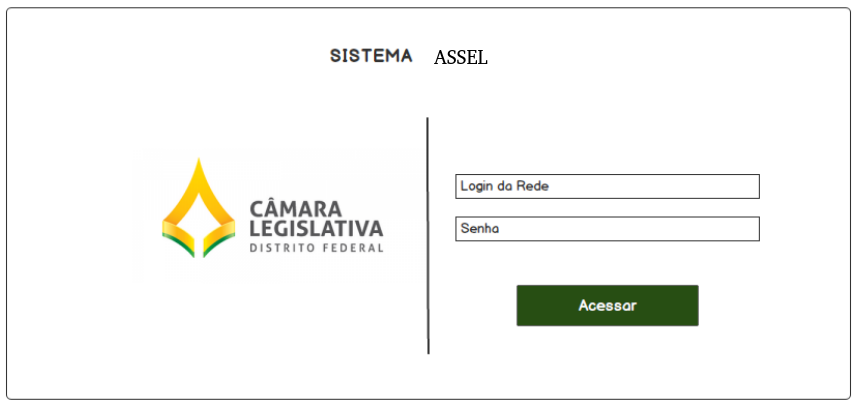
\includegraphics[width=0.8\textwidth]{fig/S1/fig-login.png}
		\caption{Tela de Login Principal}
	\label{fig:login}
	\end{figure}


	\subsection{Mudanças no Gerenciar Usuário}	
	
	Um Usuário pode estar vinculado com diversas Unidades.
	
	Então não existe mais o tipo "Externo".
	
	Pedro precisa fazer algumas mudanças lá.


	\subsection{Gerenciar Perfil}	
	
	 Parece OK
	 
	\subsection{Gerenciar Ordem de Serviço}		 
	
	\begin{enumerate}
		\item Listar - Cancelar e Abortar saem e agora é só Cancelar. O sistema verifica qual é o caso e quais são as operações.
		
		\item \textbf{Incluir e Visualizar}
		
		\begin{itemize}
			\item Quero uma tela só para incluir os Anexos um de cada vez.
			
			
			A estrutura de um Artefato é:
			\begin{itemize}			
				\item Anexo (Arquivo PDF, Imagem, Video, Etc...) - User Escolhe;
				\item Quem incluiu - Sistema registra;
				\item Data e Hora da Ultima Modificação - Sistema Registra;
				\item Nivel de Acesso (Publico ou Restrito) - User Escolhe;
				\item Justificativa Legal Se Restrito - User Escolhe;
				\item Tipo de Artefato (Inicial, Final, Pensar depois em mais casos) - Sistema Define;
				\item Descrição - User Escolhe;
			\end{itemize}		
			
			
			\item Os anexos deverão ser tratados já como Artefatos do Pacote de Artefatos vinculado a essa OS.
			
			
			\item A Especificação de Trabalho deve mostrar o \textbf{Textofato} do Tipo ``Especificação de Trabalho'' mais recente.
			
			
			A estrutura de um Textofato é:
			\begin{itemize}			
				\item Texto - User Escolhe;
				\item Quem incluiu - Sistema Registra;
				\item Data e Hora da Inclusão - Sistema Registra;
				\item Tipo de Textofato - Sistema Define;
			\end{itemize}		
			
			
		\end{itemize}
	\end{enumerate}


%\section{Reunião 13 08 21 - Ronie e Gilberto}

	Pauta: Segundo Gilberto, há uma situação que ocorreu essa semana, que temos que saber se é possível nós darmos entrada diretamente para um determinado setor. Exemplo ocorrido: Memo circular para a Assessoria Legislativa que gere algum documento.
	
	\subsection{Outros itens}
		
	\mschecknao	\xspace Modelo de Termo de Cancelamento
	
	\subsubsection{Dar entrada a uma nova OS pelo Apoio}
	

		
		
		\begin{funcionalidade}{\hypertarget{r1308-1}{Funcionalidade: Dar entrada a uma nova OS pelo Apoio}}
			A funcionalidade ``Solicitar OS'' desenvolvida parte do pressuposto que o próprio Solicitante vai fazer a solicitação.
	
			Poderíamos resolver isso fazendo uma nova funcionalidade ``Solicitar OS'' exclusiva para o pessoal do Apoio.
			
			Ela terá elementos parecidos com o outro, só que haverá a possibilidade do Apoio mesmo incluir informações.
			
			
			Temos que pegar exemplos disso para modelar ou talvez aproveitar o que já está modelado.
		\end{funcionalidade}

		
	

\chapter{Ajustes}

\section{Reunião 24 08 21 - Ronie e Gilberto}

\subsection{Codificação das OSs}

Gilberto me envia tabela contendo forma de nomear os arquivos.

Estou pensando se adotamos o mesmo modelo para nomear as OSs.

%\begin{pergunta}[1]{Muda?}
%	Esse nome pode mudar? Pode!
%\end{pergunta}

Esse nome pode mudar? 

Pode mudar. Por isso isso não pode ser usado como chave primária.


\subsection{Outros}

% >> Ver modelo do Termo de Cancelamento


% \TODO{Passar para Pedro novo campo no Solicitar OS}

% \TODO{Preciso escrever como esses códigos devem funcionar.}


	


\part{PLANEJAMENTO FUTURO}

\chapter{Planejamento Futuro}

\section{Tela de Gerenciamento de Configurações}

Configurações Identificadas:

\begin{itemize}
	\item url do sei;

	\item numero do processo;

	\item numero do documeto de solicitao;

	\item numero do documento de anexo;
\end{itemize}

os numeros atuais estao na pasta de figuras.



\section{Plano}

Esses 4 ficaram na 1 Sprint:

Login/Logout
Gerenciar Usuário
Gerenciar Perfil
Solicitar Ordem de Serviço

Gerenciar Unidades tem que estar na Próxima


Importante:
Gerenciar Ordens de Serviço


Fazer juntos:
Gerenciar Pacotes de Artefatos
Gerenciar Artefatos


Log e Auditoria por último



\section{Telas que serão necessárias}

Ver modelagem-telas que estou criando. 

\begin{itemize}
	\item Duas telas para a ASSEL

	\begin{itemize}
		\item Tela para Analisar (e aprovar) OSs;
		\item Tela para Aprovar OSs Analisadas;
	\end{itemize}
		
	Temos aqui dois Papéis: O Apoio e o Chefe.	

	\begin{itemize}
		\item Chefe = Perfil de Supervisor
		\item Apoio = Perfil de Apoio
	\end{itemize}

	
	
	
	
	
	


\end{itemize}




\section{Tela Principal da ASSEL}

Penso numa tela onde haverá um tabela contendo as OSs que \emph{estão} na ASSEL aguardando providências.

Então temos um ``Estado Interno'' da ASSEL ou ``Classes'' da OS que podem ser:


Classes das OSs dentro da ASSEL:
\begin{itemize}
	\item \textbf{Recebida} ou \textbf{Para Analisar} - OSs recebidas na ASSEL e que aguardam uma providência.
	
	Dentro dessa Classe temos as Subclasses baseadas em \emph{De onde a OS veio?} e para isso, as Subclasses fariam com que as Linhas da Tabela tivessem cores.
	
	\begin{itemize}
		\item Vermelho - OS chegou na ASSEL originando-se de um Solicitante;
		\item Amarelo - OS chegou na ASSEL pela via do ``Retorno'' de uma das Unidades Internas (UDA, Etc...);
		\item Verde - OS chegou na ASSEL pela via da ``Conclusão'' de uma das Unidades Internas (UDA, Etc...);
	\end{itemize} 
	
	
	\item \textbf{Para Cancelar} - Trata de OS já analisada e assumiu o estado ``Para Cancelar''. A linha da tabela ainda tem a cor da subclasse original, contudo, a fonte torna-se negrito. Essa OS precisa receber o consentimento do ``Perfil de Chefe'' da ASSEL para que, de fato, a OS seja cancelada e siga para frente.
	
	\item \textbf{Para Pendência} - Trata de OS já analisada e assumiu o estado ``Para Pendencia''. A linha da tabela ainda tem a cor da subclasse original, contudo, a fonte torna-se negrito. Essa OS precisa receber o consentimento do ``Perfil de Chefe'' da ASSEL para que, de fato, a OS siga seu caminho.
	
	\item \textbf{Para Distribuir} - Idem.
	
	\item \textbf{Para Entregar} - Idem.	
	
	
\end{itemize}


Outra forma de classificar as OSs dentro da ASSEL e, portanto separá-las, são em OSs não analisadas, e OSs analisadas e esperando aprovação do ``Perfil de Chefe''.

Podemos criar duas Telas separadas. 

Na primeira estarão as OSs não analisadas. Na outra, as OSs analisadas e aguardando aprovação para seguir seu caminho.

Na primeira, cujo acesso será do Apoio, contem as OSs não analisadas. De forma que o apoio possa analisar e dar um destino a elas até que a tabela fique sem nada. O trabalho do Apoio é justamente analisar OSs dessa tabela.

Na outra, acessa somente quem tem o ``Perfil de Chefe'' e o objetivo é verificar a análise que foi feita aprovando ou não a análise feita e dando seguimento às OSs.

















\section{Backlog Futuro}

\hypertarget{backlog}{Backlog}

Aqui vou adicionando funcionalidades pedidas pelos usuários que deverão se tornar funcionalidades para o futuro.

\begin{itemize}
	\item \mschecknao \xspace \hyperlink{r1308-1}{Capacidade do Apoio fazer OS em nome de outro Solicitante}
	
	\item \mschecknao \xspace \hyperlink{r160522-1}{Evolução: Campo Deputado e Orgao do SOS já vem pré-preenchido}
	
	
	
	
	
	
	
\end{itemize}














\chapter{Planejamento dos Perfis}

\section{Unidade ASSEL}

	\subsection{Perfil ASSEL Supervisor}
	
	Esse é o perfil do Chefe da Assel (e quem mais ele quiser).
	
	
	\subsection{Perfil ASSEL Apoio}
	
	Esse é o perfil de quem trabalha na Assel com o Apoio.

\section{Unidades Internas}

São os Perfis para Usuários membros das Unidades Internas da ASSEL: UDA, etc...


	\subsection{Perfil Unidade Supervisor}
	
	São os Chefes das Unidades (e quem mais eles indicarem).

	\subsection{Perfil Unidade Consultor Legislativo Elaborador}
	
	São os Consultores Legislativos que trabalham com a Elaboração de Artefatos.
	
	\subsection{Perfil Unidade Consultor Legislativo Revisor}
	
	São os Consultores Legislativos que trabalham com a Revisão de Artefatos.
	
	\subsection{Perfil Unidade Consultor Legislativo}
	
	Fazem o mesmo que os dois perfis anteriores, isto é, Perfil Unidade Consultor Legislativo Elaborador e Perfil Unidade Consultor Legislativo Revisor.
		
	\begin{imagine}{Consultores Legislativos}
		Normalmente, os Consultores Legislativos terão ambos os Perfis de Elaboradores e Revisores.
	\end{imagine}

	\begin{funcionalidade}{CL que puxam ou nao OSs}
		Terá que ter Perfis capazes de puxar OSs ou não.
	\end{funcionalidade}
	
	\begin{funcionalidade}[1]{Inserir Tipo de Unidade Dentro do Ger Perfil}
		Talvez seria bom classificar os Perfis Por Tipo com os seguintes tipos: ASSEL, INTERNO e SOLICITANTE. 
		
		Não vamos fazer assim.		
	\end{funcionalidade}
	

	\begin{funcionalidade}[1]{Caixa de Ajuda em baixo da tela}
		Inserir uma caixa de ajuda embaixo da tela.
		
		Por enquanto vou descartar isso.
	\end{funcionalidade}

	
	
\section{Unidades Externas = Solicitantes}	

São os Perfis de Unidades Solicitantes.

	\subsection{Perfil Solicitante Supervisor}
	
	São usuários capazes de fazer solicitações e, principalmente, \textbf{incluir e remover novos usuários da sua unidade} e \textbf{escolher para eles dentre os perfis possíveis}: Supervisor, Normal e Restrito.
	
	\subsection{Perfil Solicitante Normal}
	
	São os demais Solicitantes do sistema capazes de fazer tudo exceto incluir novos usuários na unidade.	
	
	\subsection{Perfil Solicitante Restrito}
	
	São usuários com o Perfil mais restrito capaz de ver os estados das OSs mas não conseguem fazer Solicitação de OSs nem tampouco cancelar OSs. Eles apenas veem.
	
	
	
	

	







\chapter{Funcionalidades Futuras}

\begin{table}[!h]
	\begin{center}
		\begin{tabular}{|p{0.4\textwidth}|c|c|}
			\hline
			\rowcolor{corCOULD!50} \multicolumn{3}{|c|}{\Large Legenda \normalsize} \\ \hline \hline
			% CABEÇALHO        
			\rowcolor{lightgray}\textbf{Estado} & \textbf{Sigla} & \textbf{Ícone} \\ \hline
			% CONTEÚDO
			% Código escrito manualmente
			\rowcolor{corCOULD!10} Requisitos a Levantar & RLN  & \msrln \\ \hline
			\rowcolor{corCOULD!20} Requisitos Levantado & RLS & \msrls \\ \hline
			\rowcolor{corCOULD!10} Requisito Novo a Aprovar & RLV & \msrlv \\ \hline
			\rowcolor{corCOULD!20} Funcionalidade Construída & FCS & \msfcs \\ \hline
			\rowcolor{corCOULD!10} Funcionalidade Não Construída & FCN & \msfcn \\ \hline
		\end{tabular}    
		\caption{\label{tab:legenda:funcionalidades} Legendas de Funcionalidades.}
	\end{center}
\end{table}

% Requisito Levantado Sim / Não / Novo
% Funcionalidade Construida Sim / Não


\section{Login/Logout \msfcn - TODOS}

\section{Gerenciar Usuário \msrls - ADM/APOIO DA ASSEL}

	\subsection{Listar}
	
	Sigla
	
	Nome Completo
	
	Divisão: Interna ou Externa
	
	Quantidade de Usuários Participantes
	
		
	\subsection{Incluir}
	\subsection{Editar}
	\subsection{Visualizar}
	\subsection{Excluir}
	\subsection{Pesquisar}
	\subsection{Vincular Perfil}


\section{Gerenciar Perfil \msrls - ADM DA ASSEL}


	\subsection{Listar}
	\subsection{Incluir}
	\subsection{Editar}
	\subsection{Visualizar}
	\subsection{Excluir}
	\subsection{Pesquisar}


\section{Solicitar Ordem de Serviço \msfcn - SOLICITANTE}



	\subsection{Listar}

	\subsection{\textcolor{red}{Incluir pelo Solicitante} \msrls}
	
	Esse é o original.
	
	
	\begin{evolutivo}[1]{\hypertarget{r160522-1}{Evolução: Campo Deputado e Orgao já vem pré-preenchido}}
		\begin{itemize}
			\item Juliana deu essa idéia e vale a pena acatar.
			\item Isso é uma coisa que deverá ser alterada depois em alguma Sprint no futuro.
			\item Coloquei isso no \hyperlink{backlog}{backlog}.
		\end{itemize}
		\tcblower		
		\begin{itemize}
			\item No Solicitar Ordem de Serviço, no formulário de criação de nova OS, existe o Campo ``Deputado/Orgao'' que está livre para o usuário escolher o que quer.
		
			\item 	O ideal é que isso não seja possível pois o ``Deputado/Orgao'' é aquele escolhido no ComboBox de Unidades.
			
			\item 	Ou seja, isso terá de ser alterado lá para que venha já pré-preenchido sem capacidade de ser Editado.
			
			\item Repassei isso para o Robson na reunião de 05 de Setembro 2022.	
		\end{itemize}
	\end{evolutivo}
	

	
	\subsection{\textcolor{red}{Incluir pelo Apoio} \msrlv}
	
	Esse foi pedido pelo Gil, mas ainda não foi feito pela Fábrica.
	
	\subsection{Visualizar}
	\subsection{Cancelar}
	
	
	
	%\toPedro{Melhorar Solicitar OS - Parte de como funciona no SEI} RESOLVIDO
	
	
	\begin{enumerate}
		\item Processo é gerado na Unidade do Sei pertencente ao Solicitante.
	
		\item 	O Arquivo da OS é gerado junto com os anexos e espera-se que ele seja assinado.
		
		\item 	Depois que é assinado, nada mais é feito.
		
		\item 	O sistema manda o processo para a ASSEL.
		
		\item 	Recebe na ASSEL, coloca um Acompanhamento Especial (ou algo assim) e arquiva (ou nao). Esse comportamento tem que ser conversado com o Gilberto.	

		%\toGil{Qual comportamento deve ocorrer?} RESOLVIDO

	\end{enumerate}
	

	
		
	%\TODO{Vai precisar editar OS para incluir anexos caso ocorra pendencia}.	RESOLVIDO
	
	
	
\section{\textcolor{red}{Gerenciar Usuários do Solicitante} \msrlv - SOLICITANTE}

\begin{funcionalidade}{Tela Gerenciar Usuários do Solicitante}
	Vai ter que ter essa tela no futuro.
\end{funcionalidade}

Essa tela deve estar disponível por cada Solicitante para que eles possam gerenciar seus próprios usuários.



	

\section{Gerenciar Unidades \msrln - ADM/APOIO ASSEL}


	\begin{nota}{Novas Eleições}
		Futuramente, essa Gerenciar Unidade pode ter de passar por algumas revisões para comportar a característica de coisas que podem ser necessárias quando ocorrem eleições.
		
		O vínculo dos Gabinetes é com os Deputados.
		
		Talvez seja necessário ATIVAR e DESATIVAR unidades inteiras. Ou seja, um Deputado que saiu terá sua unidade de seu Gabinete desativado e poderá ser reativado depois, caso reeleito no futuro, e assim terá de volta o histórico de Solicitações feitas por ele.
		
		Aqui é importante ressaltar que pode-se perder o vínculo com o SEI.
		
		O ideal é perguntar para o Jefferson como isso será feito no SEI e talvez espelhar o comportamento para o sistema.				
	\end{nota}
		
		
	\begin{nota}{Novas Eleições}		
		Ao conversar com o Gilberto, ele diz que o histórico do solicitante no caso de ser Gabinete é atrelado ao Deputado. 
		
		Assim, o Deputado tem uma pasta. 
		
		Seria bom ver com o Jefferson mesmo assim como isso se dará no SEI.
	\end{nota}

	%\TODO{Perguntar isso ao Jefferson}
	
	
	O negócio vai ser vincular os Gabinetes aos Deputados. Fazer uma tabela separada de Deputados e vincular eles 1 a 1. É uma forma.	


	\subsection{Listar}
	
	SIGLA
	
	NOME
	
	Divisão
	
	Quantidade de Usuários Ativos Vinculados à Unidade
	
	
	\subsection{Incluir}
	
	Elas terão que vir do SEI.
	
	Inclusão Individual: Lista com campo de pesquisa.
	
	Seleciona apenas 1.
	
	Combobox \emph{Origem} com 2 Opções: Externo Interno
	Externo é o Default
	
	Salvar	
	
	Tem que ter vinculação com a Unidade do SEI.
	
	Não pode criar a Unidade Duas Vezes;
	
	
	\subsection{Editar}
	
	Permitindo Ações
	
	
	
	
	\subsection{Visualizar}
	
	Não permitiria Ação
	
	
	Nome
	
	Sigla
	
	Origem: Interno ou Externo
	
	%\TODO[1]{Mudar o nome da divisão}
	% Eu desisti de mudar esse nome. Vou deixar divisão. Virou origem.	
		
	Apresentar a Lista de Usuários Vinculados Áquela Unidade
	
	Filtro
	
	Ativar / Desativar aqui nessa Visualização
	
	Desvincular dessa Unidade () Não
	
	Imprimir um PDF  (Usuários Ativos da Unidade)
	
	
	% \TODO{Fazer padrão de como seria o pdf com isso.}	
	
	\subsection{Excluir}
	
	Não pode excluir se tiverem usuários vinculados à Unidade.
	
	Inicialmente tornar impossível excluir as Unidades Internas que já devem vir pré-cadastradas.
	
	\subsection{Pesquisar}

	Filtro da Lista



	% \TODO{Ver questão da eleição - O que acontece com os Gabinetes?} Já tem TODO para isso.
	
	%\TODO{Questão de ter usuários sem unidade.} Já está nos ajustes.
	
	
	

\section{Gerenciar Ordens de Serviço da Assel \msrln - ASSEL}
\label{tela:ger-os-assel}

	Reuniões: \ref{reuniao:r200921}.
	
	Ver detalhamento em \ref{detalhes:ger-os-assel}.
	

	\subsection{Listar}
		Ver Protótipo que fiz no Google SpreadSheets.
		
		Listar vai ter os campos:
		
		\begin{env-cor}{Campos Associados à Solicitação}{blue}
			\begin{itemize}
				\item Solicitação
				\item Unidade Solicitante
				\item Tipo
				\item Subtipo
				\item Urgente
			\end{itemize}
		\end{env-cor}
		
		\begin{env-cor}{Informações Enviadas Pelo Remetente}{cyan}
			\begin{itemize}
				\item Remetente
				\item Assunto	
			\end{itemize}
		\end{env-cor}
				
		\begin{env-cor}{Somente Aqui na ASSEL}{orange}
			\begin{itemize}
				\item Atribuição
				\item Análise
				\item Destino
				\item Ação	
			\end{itemize}
		\end{env-cor}


		Vou descrever cada coluna:

		\subsubsection{Solicitação} 
			Contém o código único da Solicitação.
		\subsubsection{Unidade Solicitante} 
			Unidade Solicitante
		\subsubsection{Tipo} 
			Tipo
		\subsubsection{Subtipo} 
			Subtipo
		\subsubsection{Urgente} 
			Atributo da Solicitação que ainda não tinha aparecido nas especificações porque somente aqui na ASSEL que ele é definido.
			
			Urgente é um atributo booleano (SIM/NÃO). Default é Não.
			
			Aqui na ASSEL é que o Apoio vai definir se uma Solicitação é Urgente ou não.			
		\subsubsection{Remetente} 
			Última unidade onde tramitou a Solicitação antes de chegar aqui na ASSEL.
		\subsubsection{Assunto} 
			Nesse sistema, todo trâmite de solicitações terá associado uma mensagem (digitada pelo usuário) com um assunto. Os assuntos serão definidos pelo sistema.
			
		\subsubsection{Atribuição} 			
		
			Default: Não Atribuído.
			
			Toda vez que uma Solicitação é enviada para a ASSEL, esse campo é mantido.
			

			
		\subsubsection{Análise}
			
			Default: Não Analisado.			
			
			Toda vez que uma Solicitação é enviada para a ASSEL, esse campo é resetado para Não Analisado.
			
			As opções para Usuários são: Cancelar, Pendencia, Distribuir. Mas o campo ainda pode receber o valor Não Se Aplica.
			
		\subsubsection{Destino}			
		
			Default: Não Especificado.
				
			Toda vez que uma Solicitação é enviada para a ASSEL, esse campo é resetado para Não Especificado.
			
			As opções são: Enviar para UDA, USE...
			
			
		\subsubsection{Ação}			
		
			Ação é um resultado de uma regra aplicada sobre os campos Análise e Destino.
			
		
		
		
		% \TODO{Falar que tem que ter 2 popups: Ementa ou Especificação do Trabalho e Texto do Remetente} RESOLVIDO

		% \TODO{Falar do Memo Texto da Análise} Está previsto.
		
		% \TODO{Especificar as funcionalidades} Está especificado.
	
	\subsection{Editar}

	\begin{itemize}
		\item Atribuir Urgência
		\item Atribuir Servidor  - Forma de Atribuir a Solicitação a um determinado Usuário da Unidade ASSEL.
		\item Atribuir Análise
		\item Atribuir Destino
		\item Executar Ação
	\end{itemize}	


	%\begin{funcionalidade}[1]{Não esquecer disso - Funcionalidades}
	
	% Em algum lugar aqui deve ter que ser possível adicionar novos arquivos na Solicitação.
		
	% Deve ser possível também adicionar ``Anotações'' na Solicitação.
		
	% Deve ser possível vincular uma Solicitação a Outras.
	
	% Talvez o lugar para fazer essas coisas acima seja dentro da tela de Analisar.
	
	% Resolvido
	
	%\end{funcionalidade}

	
	





	\subsection{Visualizar}

	Vai mostrar todos os detalhes da Solicitação.
	
	Aqui deve ser possível inserir novos Anexos (Artefatos) à Solicitação. Artefatos incluídos aqui deverão ser classificado com o tipo ``ASSEL''.
	 

	\subsection{Pesquisar}
	\subsection{Filtrar}
	\subsection{Gerar Relatório}


\section{\red{Gerenciar Ordens de Serviço das Unidades} \msrlv - UNIDADES}

\TODO{A gente só vai se preocupar com isso depois de corrigir os defeitos e deixar tudo funcionando.}








\section{Gerenciar Pacotes de Artefatos \msrln}


	\subsection{Listar}
	\subsection{Incluir}
	\subsection{Excluir}
	\subsection{Pesquisar}
	
	Essa funcionalidade é uma das mais importantes pois acho que aqui devemos fazer a pesquisa textual dentro dos artefatos.



\section{Gerenciar Artefatos \msrln}


	\subsection{Listar}
	\subsection{Incluir}
	\subsection{Editar}
	\subsection{Excluir}
	\subsection{Pesquisar}


\section{Log e Auditoria \msrln}


	\subsection{Pesquisar}


\chapter{Telas Adicionais}


\section{Tela de Pesquisa de Artefatos \msrln}






\part{RESUMO}


\chapter{Ambientes}
\newcounter{CounterAmbientes}

\TODO{Último}

\toGil{Último}

\toPedro{Último}

\begin{pergunta}{Última}
	Última
\end{pergunta}

\begin{resposta}{Última}
	Última
\end{resposta}

\begin{importante}{Última}
	Última
\end{importante}

\begin{requisito}{Última}
	Última
\end{requisito}

\begin{funcionalidade}{Última}
	Última
\end{funcionalidade}

\begin{exemplo}{Última}
	Última
\end{exemplo}

\begin{nota}{Última}
	Última
\end{nota}

\begin{imagine}{Última}
	Última
\end{imagine}

\begin{ajuste}{Último}
	Última
\end{ajuste}

\begin{falha}[1]{Último}
	Antes
	\tcblower
	Depois
\end{falha}


\begin{falha}[0]{Último}
	Antes
	\tcblower
	Depois
\end{falha}

\begin{evolutivo}[0]{Último}
	Evolutivo
\end{evolutivo}


Resumo dos principais \hypertarget{TargetResumoAmbientes}{ambientes}:

\section{Afazeres}

Afazeres é qualquer manifestação de algo que precisa ser feito em algum momento. Não sei ainda aonde se encaixa mas precisos deixar escrito para não esquecer e depois eu reavalio esse afazer.

\subsection{Gerais}

\listarAmbiente[TargetTodo]{\ListaTodo}

\subsection{Para Gilberto}

\listarAmbiente[TargetTogil]{\ListaTogil}

\subsection{Para Pedro}

\listarAmbiente[TargetTopedro]{\ListaTopedro}

\section{Perguntas}

São dúvidas e perguntas que preciso fazer para alguém me responder. Geralmente esse alguém é o Líder de Negócios ou integrantes da área de negócios.

\listarAmbiente[TargetPergunta]{\ListaPergunta}

\section{Respostas}

São respostas às perguntas. Deixo registrado.

\listarAmbiente[TargetResposta]{\ListaResposta}

\section{Importante}

Qualquer coisa que queira destacar como importante.

\listarAmbiente[TargetImportante]{\ListaImportante}

\section{Requisitos}

Nascem dentro das entrevistas.

\listarAmbiente[TargetRequisito]{\ListaRequisito}

\section{Funcionalidades}

Já são declarações mais consolidadas de coisas que precisam acontecer.

\listarAmbiente[TargetFuncionalidade]{\ListaFuncionalidade}

\section{Exemplos}

Exemplo de algo.

\listarAmbiente[TargetExemplo]{\ListaExemplo}

\section{Nota}

Notas sobre qualquer coisa.

\listarAmbiente[TargetNota]{\ListaNota}

\section{Imagine}

Descrição de uma possibilidade. Um cenário para servir de inspiração.

\listarAmbiente[TargetImagine]{\ListaImagine}


\section{Ajustes}

Preocupações relacionadas a coisas já desenvolvidas e que podem levar a erros. 

\listarAmbiente[TargetAjuste]{\ListaAjuste}


\section{Falhas}

Falhas encontradas nos testes.

\listarAmbiente[TargetFalha]{\ListaFalha}

\section{Evolutivos}

São funcionalidades evolutivas identificadas.

\listarAmbiente[TargetEvolutivo]{\ListaEvolutivo}







% \chapter{Testes}

\begin{pergunta}{Teste 1}
	Pergunta 1
\end{pergunta}

\begin{pergunta}{Teste 2}
	Pergunta 2
\end{pergunta}

\begin{pergunta}{Teste 3}
	Pergunta 3
\end{pergunta}

\begin{pergunta}{Teste 4}
	Pergunta 4
\end{pergunta}


\begin{resposta}{Teste 1}
	Resposta 5
\end{resposta}


\printlista{\perglista}

Separa

\printlista{\resplista}





% define few variables that hold some value
\def\One{this is one}
\def\Two{this is two}
\def\Three{this is three}

% add the above commands to a list named `CmdList'
\listcsgadd{CmdList}{One}
\listcsgadd{CmdList}{Two}
\listcsgadd{CmdList}{Three}

% Now loop-over them to print their values
\begin{description}
	\renewcommand*{\do}[1]{\item[#1:] \csuse{#1}}
	\dolistcsloop{CmdList}
\end{description}    

% creating a table needs little bit more trickery; You cannot insert table entries directly.
% You first have to accumulate all table data into some temporary variable and then use that.
\begingroup
\newcommand\tablecontent{}
\def\do#1{\appto\tablecontent{\hline \textbf{#1} & \csuse{#1}\\}}%
\dolistcsloop{CmdList} % collect the data in a table format
\begin{tabulary}{\textwidth}{|L|L|} % now print the collected data 
	\tablecontent \hline
\end{tabulary}              
\endgroup

\section{Funcionalidades}


\setcounter{CounterFuncionalidade}{0}
\begin{itemize}
	\renewcommand*{\do}[1]{\item #1}
	\dolistcsloop{ListaFuncionalidade}
\end{itemize}   


%\hyperlink{TargetFuncionalidade\arabic{CounterFuncionalidade}}{#1}

separa

\setcounter{CounterFuncionalidade}{0}
\begin{itemize}
	\forlistloop{\stepcounter{CounterFuncionalidade} \item \hyperlink{TargetFuncionalidade\arabic{CounterFuncionalidade}}}{\ListaFuncionalidade}
\end{itemize}

%Posso fazer um novo counter aqui e vai funcionar


\hypertarget{TA}{Aqui}

\begin{envteste}[1]{Titulo}
Deu verdade = Foi feito + Nao entra na lista
\end{envteste}
 


\begin{envteste}{Titulo}
Deu falso = Nao foi feito = Entra na lista
\end{envteste}



\section{Comando Novo}

\begin{importante}{Importante 1}
	Teste
\end{importante}


\begin{importante}{Importante 2}
	Teste
\end{importante}


\begin{importante}{Importante 3}
	Teste
\end{importante}


\begin{importante}{Importante 4}
	Teste
\end{importante}


\begin{importante}{Importante 5}
	Teste
\end{importante}


%\setcounter{CounterImportante}{0}
%\begin{itemize}
%	\forlistloop{\stepcounter{CounterImportante} \item %\hyperlink{TargetImportante\arabic{CounterImportante}}}{\ListaImportante}
%\end{itemize}



\setcounter{CounterAmbientes}{0}
\begin{itemize}
	\forlistloop{\stepcounter{CounterAmbientes} \item \hyperlink{TargetFuncionalidade\arabic{CounterAmbientes}}}{\ListaFuncionalidade}
\end{itemize}


\setcounter{CounterFuncionalidade}{0}
\begin{itemize}
	\forlistloop{\stepcounter{CounterFuncionalidade} \item \hyperlink{TargetFuncionalidade\arabic{CounterFuncionalidade}}}{\ListaFuncionalidade}
\end{itemize}

Separa

%\setcounter{CounterAmbientes}{0}
%\begin{itemize}
%	\forlistloop{\stepcounter{CounterAmbientes} \item %\hyperlink{TargetImportante\arabic{CounterAmbientes}}}{\ListaImportante}
%\end{itemize}


% ####
% DESENVOLVIMENTO
% ####

% Aqui você coloca os .tex na ordem que serão compilados
% Pode usar os comandos parte para dividir em partes se quiser

\part{PLANEJAMENTO}

\chapter{Afazeres}


\TODO{Aqui todos}


\section{Afazeres Gerais}

\TODO{Qualquer todo}





\chapter{Diário}

\section{26 Nov 2023}

Criei esse ambiente latex a partir de al para escrever alguma documentação.

\part{MODELAGEM}

\chapter{Passos Fundamentais}

Temos:

\begin{itemize}
	\item ABR - Abre;
	\item JUN - Junta;
	\item FRT - Frente;
	\item TRS - Trás;
	\item LUG - Lugar;
\end{itemize}

E:

\begin{itemize}
	\item JCF - Junta Cruzando à Frente;
	\item JCT - Junta Cruzando Atrás;
\end{itemize}

E:

\begin{itemize}
	\item ABF - Abre indo à Frente;
	\item ABT - Abre indo à Trás;
	\item FCF - Frente Cruzando à Frente;
	\item TCT - Tráz Cruzando à Traz;
\end{itemize}




\part{RESUMO}

\chapter{Ambientes}
\newcounter{CounterAmbientes}

\TODO{Último}

\toGil{Último}

\toPedro{Último}

\begin{pergunta}{Última}
	Última
\end{pergunta}

\begin{resposta}{Última}
	Última
\end{resposta}

\begin{importante}{Última}
	Última
\end{importante}

\begin{requisito}{Última}
	Última
\end{requisito}

\begin{funcionalidade}{Última}
	Última
\end{funcionalidade}

\begin{exemplo}{Última}
	Última
\end{exemplo}

\begin{nota}{Última}
	Última
\end{nota}

\begin{imagine}{Última}
	Última
\end{imagine}

\begin{ajuste}{Último}
	Última
\end{ajuste}

\begin{falha}[1]{Último}
	Antes
	\tcblower
	Depois
\end{falha}


\begin{falha}[0]{Último}
	Antes
	\tcblower
	Depois
\end{falha}

\begin{evolutivo}[0]{Último}
	Evolutivo
\end{evolutivo}


Resumo dos principais \hypertarget{TargetResumoAmbientes}{ambientes}:

\section{Afazeres}

Afazeres é qualquer manifestação de algo que precisa ser feito em algum momento. Não sei ainda aonde se encaixa mas precisos deixar escrito para não esquecer e depois eu reavalio esse afazer.

\subsection{Gerais}

\listarAmbiente[TargetTodo]{\ListaTodo}

\subsection{Para Gilberto}

\listarAmbiente[TargetTogil]{\ListaTogil}

\subsection{Para Pedro}

\listarAmbiente[TargetTopedro]{\ListaTopedro}

\section{Perguntas}

São dúvidas e perguntas que preciso fazer para alguém me responder. Geralmente esse alguém é o Líder de Negócios ou integrantes da área de negócios.

\listarAmbiente[TargetPergunta]{\ListaPergunta}

\section{Respostas}

São respostas às perguntas. Deixo registrado.

\listarAmbiente[TargetResposta]{\ListaResposta}

\section{Importante}

Qualquer coisa que queira destacar como importante.

\listarAmbiente[TargetImportante]{\ListaImportante}

\section{Requisitos}

Nascem dentro das entrevistas.

\listarAmbiente[TargetRequisito]{\ListaRequisito}

\section{Funcionalidades}

Já são declarações mais consolidadas de coisas que precisam acontecer.

\listarAmbiente[TargetFuncionalidade]{\ListaFuncionalidade}

\section{Exemplos}

Exemplo de algo.

\listarAmbiente[TargetExemplo]{\ListaExemplo}

\section{Nota}

Notas sobre qualquer coisa.

\listarAmbiente[TargetNota]{\ListaNota}

\section{Imagine}

Descrição de uma possibilidade. Um cenário para servir de inspiração.

\listarAmbiente[TargetImagine]{\ListaImagine}


\section{Ajustes}

Preocupações relacionadas a coisas já desenvolvidas e que podem levar a erros. 

\listarAmbiente[TargetAjuste]{\ListaAjuste}


\section{Falhas}

Falhas encontradas nos testes.

\listarAmbiente[TargetFalha]{\ListaFalha}

\section{Evolutivos}

São funcionalidades evolutivas identificadas.

\listarAmbiente[TargetEvolutivo]{\ListaEvolutivo}







%\part{Part One}

%----------------------------------------------------------------------------------------
%	CHAPTER 1
%----------------------------------------------------------------------------------------

\chapterimage{chapter_head_2.pdf} % Chapter heading image

\chapter{Text Chapter}

\section{Paragraphs of Text}\index{Paragraphs of Text}

\lipsum[1-7] % Dummy text

%------------------------------------------------

\section{Citation}\index{Citation}


\TODO{Teste}

\TODO{Teste}

\begin{env-cinza}
    Teste de Ambiente
\end{env-cinza}

\begin{envtodo}{Todo}
    Teste de Ambiente
\end{envtodo}



This statement requires citation \cite{article_key}; this one is more specific \cite[162]{book_key}.

%------------------------------------------------

\section{Lists}\index{Lists}

Lists are useful to present information in a concise and/or ordered way\footnote{Footnote example...}.

\subsection{Numbered List}\index{Lists!Numbered List}

\begin{enumerate}
\item The first item
\item The second item
\item The third item
\end{enumerate}

\subsection{Bullet Points}\index{Lists!Bullet Points}

\begin{itemize}
\item The first item
\item The second item
\item The third item
\end{itemize}

\subsection{Descriptions and Definitions}\index{Lists!Descriptions and Definitions}

\begin{description}
\item[Name] Description
\item[Word] Definition
\item[Comment] Elaboration
\end{description}

%----------------------------------------------------------------------------------------
%	CHAPTER 2
%----------------------------------------------------------------------------------------

\chapter{In-text Elements}

\section{Theorems}\index{Theorems}

This is an example of theorems.

\subsection{Several equations}\index{Theorems!Several Equations}
This is a theorem consisting of several equations.

\begin{theorem}[Name of the theorem]
In $E=\mathbb{R}^n$ all norms are equivalent. It has the properties:
\begin{align}
& \big| ||\mathbf{x}|| - ||\mathbf{y}|| \big|\leq || \mathbf{x}- \mathbf{y}||\\
&  ||\sum_{i=1}^n\mathbf{x}_i||\leq \sum_{i=1}^n||\mathbf{x}_i||\quad\text{where $n$ is a finite integer}
\end{align}
\end{theorem}

\subsection{Single Line}\index{Theorems!Single Line}
This is a theorem consisting of just one line.

\begin{theorem}
A set $\mathcal{D}(G)$ in dense in $L^2(G)$, $|\cdot|_0$. 
\end{theorem}

%------------------------------------------------

\section{Definitions}\index{Definitions}

This is an example of a definition. A definition could be mathematical or it could define a concept.

\begin{definition}[Definition name]
Given a vector space $E$, a norm on $E$ is an application, denoted $||\cdot||$, $E$ in $\mathbb{R}^+=[0,+\infty[$ such that:
\begin{align}
& ||\mathbf{x}||=0\ \Rightarrow\ \mathbf{x}=\mathbf{0}\\
& ||\lambda \mathbf{x}||=|\lambda|\cdot ||\mathbf{x}||\\
& ||\mathbf{x}+\mathbf{y}||\leq ||\mathbf{x}||+||\mathbf{y}||
\end{align}
\end{definition}

%------------------------------------------------

\section{Notations}\index{Notations}

\begin{notation}
Given an open subset $G$ of $\mathbb{R}^n$, the set of functions $\varphi$ are:
\begin{enumerate}
\item Bounded support $G$;
\item Infinitely differentiable;
\end{enumerate}
a vector space is denoted by $\mathcal{D}(G)$. 
\end{notation}

%------------------------------------------------

\section{Remarks}\index{Remarks}

This is an example of a remark.

\begin{remark}
The concepts presented here are now in conventional employment in mathematics. Vector spaces are taken over the field $\mathbb{K}=\mathbb{R}$, however, established properties are easily extended to $\mathbb{K}=\mathbb{C}$.
\end{remark}

%------------------------------------------------

\section{Corollaries}\index{Corollaries}

This is an example of a corollary.

\begin{corollary}[Corollary name]
The concepts presented here are now in conventional employment in mathematics. Vector spaces are taken over the field $\mathbb{K}=\mathbb{R}$, however, established properties are easily extended to $\mathbb{K}=\mathbb{C}$.
\end{corollary}

%------------------------------------------------

\section{Propositions}\index{Propositions}

This is an example of propositions.

\subsection{Several equations}\index{Propositions!Several Equations}

\begin{proposition}[Proposition name]
It has the properties:
\begin{align}
& \big| ||\mathbf{x}|| - ||\mathbf{y}|| \big|\leq || \mathbf{x}- \mathbf{y}||\\
&  ||\sum_{i=1}^n\mathbf{x}_i||\leq \sum_{i=1}^n||\mathbf{x}_i||\quad\text{where $n$ is a finite integer}
\end{align}
\end{proposition}

\subsection{Single Line}\index{Propositions!Single Line}

\begin{proposition} 
Let $f,g\in L^2(G)$; if $\forall \varphi\in\mathcal{D}(G)$, $(f,\varphi)_0=(g,\varphi)_0$ then $f = g$. 
\end{proposition}

%------------------------------------------------

\section{Examples}\index{Examples}

This is an example of examples.

\subsection{Equation and Text}\index{Examples!Equation and Text}

\begin{example}
Let $G=\{x\in\mathbb{R}^2:|x|<3\}$ and denoted by: $x^0=(1,1)$; consider the function:
\begin{equation}
f(x)=\left\{\begin{aligned} & \mathrm{e}^{|x|} & & \text{si $|x-x^0|\leq 1/2$}\\
& 0 & & \text{si $|x-x^0|> 1/2$}\end{aligned}\right.
\end{equation}
The function $f$ has bounded support, we can take $A=\{x\in\mathbb{R}^2:|x-x^0|\leq 1/2+\epsilon\}$ for all $\epsilon\in\intoo{0}{5/2-\sqrt{2}}$.
\end{example}

\subsection{Paragraph of Text}\index{Examples!Paragraph of Text}

\begin{example}[Example name]
\lipsum[2]
\end{example}

%------------------------------------------------

\section{Exercises}\index{Exercises}

This is an example of an exercise.

\begin{exercise}
This is a good place to ask a question to test learning progress or further cement ideas into students' minds.
\end{exercise}

%------------------------------------------------

\section{Problems}\index{Problems}

\begin{problem}
What is the average airspeed velocity of an unladen swallow?
\end{problem}

%------------------------------------------------

\section{Vocabulary}\index{Vocabulary}

Define a word to improve a students' vocabulary.

\begin{vocabulary}[Word]
Definition of word.
\end{vocabulary}

%----------------------------------------------------------------------------------------
%	PART
%----------------------------------------------------------------------------------------

\part{Part Two}

%----------------------------------------------------------------------------------------
%	CHAPTER 3
%----------------------------------------------------------------------------------------

\chapterimage{chapter_head_1.pdf} % Chapter heading image

\chapter{Presenting Information}

\section{Table}\index{Table}

\begin{table}[h]
\centering
\begin{tabular}{l l l}
\toprule
\textbf{Treatments} & \textbf{Response 1} & \textbf{Response 2}\\
\midrule
Treatment 1 & 0.0003262 & 0.562 \\
Treatment 2 & 0.0015681 & 0.910 \\
Treatment 3 & 0.0009271 & 0.296 \\
\bottomrule
\end{tabular}
\caption{Table caption}
\label{tab:example} % Unique label used for referencing the table in-text
%\addcontentsline{toc}{table}{Table \ref{tab:example}} % Uncomment to add the table to the table of contents
\end{table}

Referencing Table \ref{tab:example} in-text automatically.

%------------------------------------------------

\section{Figure}\index{Figure}

\begin{figure}[h]
\centering
\includegraphics[scale=0.5]{placeholder.jpg}
\caption{Figure caption}
\label{fig:placeholder} % Unique label used for referencing the figure in-text
%\addcontentsline{toc}{figure}{Figure \ref{fig:placeholder}} % Uncomment to add the figure to the table of contents
\end{figure}

Referencing Figure \ref{fig:placeholder} in-text automatically.


%%--------------------------------------------------------------
%  Capítulos e seções
%--------------------------------------------------------------
%
% Um capítulo se inicia com o seguinte comando "\capitulo{Título}."
%
% Uma seção se inicia com o seguinte comando "\secao{Título da Seção}". Caso queira adicionar a seção ao índice acrescente o comando "\index{Título da Seção}. 
%
% O mesmo princípio é utilizado para os subníveis da seção. São eles: subseção e subsubseção, dados pelos comandos "\subsecao{Título}" e "\subsubsecao{Título}". Estes podem ser seguidos ou não do comando "\index{Título}"
%
%--------------------------------------------------------------



% Título do capítulo
\part{Exemplos}
\capitulo{Exemplos}


  Aqui fica o texto introdutório do capítulo.
  Este é o texto de um capítulo.

    % título da seção
    \secao{titulo da seção}\index{Palavra-chave}
 
        Escreva o texto da seção aqui. 
    
    
        % título da subseção
        \subsecao{titulo da subseção}
                
                Texto da seção.
        
                % título da subsubseção
                \subsubsecao{titulo da subseção}\index{palavra-chave(seção)!palavra-chave} 

                    Texto da subsubseção.

%--------------------------------------------------------------
%   Teoremas
%--------------------------------------------------------------


    \secao{Teoremas}\index{Teoremas}

        Esta seção traz exemplos de teoremas.

        \subsecao{Várias Equações}\index{Teoremas!Várias Equações}

            Exemplo de Teorema com várias equações.

            \begin{theorem}[Nome do teorema]
                In $E=\mathbb{R}^n$ all norms are equivalent. It has the properties:
                \begin{align}
                    & \big| ||\mathbf{x}|| - ||\mathbf{y}|| \big|\leq || \mathbf{x}- \mathbf{y}||\\
                    &  ||\sum_{i=1}^n\mathbf{x}_i||\leq \sum_{i=1}^n||\mathbf{x}_i||\quad\text{where $n$ is a finite integer}
                \end{align}
            \end{theorem}

        \subsecao{Linha Única}\index{Teoremas!Linha Única}
            Teorema em Linha Única.
            \begin{theorem}
                A set $\mathcal{D}(G)$ in dense in $L^2(G)$, $|\cdot|_0$. 
            \end{theorem}

%--------------------------------------------------------------


%--------------------------------------------------------------
%   Definições
%--------------------------------------------------------------
\secao{Definições}\index{Definições}

    Exemplo de Definição.
    \begin{definition}[Nova Definição]
        Given a vector space $E$, a norm on $E$ is an application, denoted $||\cdot||$, $E$ in $\mathbb{R}^+=[0,+\infty[$ such that:
        \begin{align}
            & ||\mathbf{x}||=0\ \Rightarrow\ \mathbf{x}=\mathbf{0}\\
            & ||\lambda \mathbf{x}||=|\lambda|\cdot ||\mathbf{x}||\\
            & ||\mathbf{x}+\mathbf{y}||\leq ||\mathbf{x}||+||\mathbf{y}||
        \end{align}
    \end{definition}

%--------------------------------------------------------------

%--------------------------------------------------------------
%   Notações
%--------------------------------------------------------------
\secao{Notações}\index{Notações}

    \begin{notation}
        Given an open subset $G$ of $\mathbb{R}^n$, the set of functions $\varphi$ are:
        \begin{enumerate}
            \item Bounded support $G$;
            \item Infinitely differentiable;
        \end{enumerate}
        a vector space is denoted by $\mathcal{D}(G)$. 
    \end{notation}

%--------------------------------------------------------------



%--------------------------------------------------------------
%  Indicação de ícones
%--------------------------------------------------------------
    \secao{Indicação de Ícones}\index{Indicação de Ícones}

        \mais{ Oferece novas informações que enriquecem o assunto ou “curiosidades” e notícias recentes relacionadas ao tema estudado. Não indicar simplesmente livros, filmes, links, etc. Oriente os estudantes sobre o que vão encontrar no material indicado.
        }

        \midia{ Sempre que se desejar que os estudantes desenvolvam atividades empregando diferentes mídias: vídeos, filmes, jornais, ambiente AVA, sites e outras.
        }

        \glossario{ Indica a definição de um termo, palavra ou expressão utilizada no texto.
        }

        \atividade{ Apresenta atividades em diferentes níveis de aprendizagem para que o estudante possa realizá-las e conferir o seu domínio do tema estudado.
        }

        \atencao{  Indica pontos de maior relevância no texto.
       
        o 
        
        quadro 
       
        aumenta automaticamente
      
        kkk
        }

%--------------------------------------------------------------


%--------------------------------------------------------------
%   Proposições
%--------------------------------------------------------------
    \secao{Proposições}\index{Proposições}

    Estes são exemplos de proposição.
    
        \subsecao{Várias Equações}\index{Proposições!Várias Equações}
            Exemplo com várias equações.
            \begin{proposition}[Nome da Proposição]
                It has the properties:
                \begin{align}
                    & \big| ||\mathbf{x}|| - ||\mathbf{y}|| \big|\leq || \mathbf{x}- \mathbf{y}||\\
                    &  ||\sum_{i=1}^n\mathbf{x}_i||\leq \sum_{i=1}^n||\mathbf{x}_i||\quad\text{where $n$ is a finite integer}
                \end{align}
            \end{proposition}

        \subsecao{Linha Única}\index{Proposições!Linha Única}
            Exemplo em Linha única.
            \begin{proposition} 
                Let $f,g\in L^2(G)$; if $\forall \varphi\in\mathcal{D}(G)$, $(f,\varphi)_0=(g,\varphi)_0$ then $f = g$. 
            \end{proposition}

%--------------------------------------------------------------

%--------------------------------------------------------------
%   Equações 
%--------------------------------------------------------------
    \secao{Equações}\index{Equações}
        Este é um exemplo de uma equação.
        \begin{equation}
            \cos^{2}{x} + \sin^{2}{x} = 1, \quad \forall x \in \mathbb{R}
            \label{equ:1}
        \end{equation}
        
        A equação \ref{equ:1} está referenciada.
        
        Caso não queira uma numeração para a equação:
        \begin{equation*}
            \cos^{2}{x} + \sin^{2}{x} = 1, \quad \forall x \in \mathbb{R}
        \end{equation*}       
        %Note a existência de funções como "\cos{}" e "sin{}" e não, simplismente escrito "cos()" e "sin()".
        
        Um conjunto de equações:
        
        \begin{equation}
            f(x) = 
            \begin{cases}
                2x+1, \quad  x \leq 0 \\
               x^2 +\frac{3}{2}x +\log{x},  \quad  x > 0
            \end{cases}
            \label{equ:2}
        \end{equation}   
        %Note como é criada uma fração com o comando "\frac{}{}"
        
  
       \subsecao{Matrizes}\index{Equações!Matriz}
        
         Exemplo padrão % o símbolo "&" é o separador de colunas e o "\\" indica final de linha
        
        $ %Entrando no Modo matémático entre "$$"
        \begin{bmatrix}
            1 & 2 & 3\\
            a & b & c
        \end{bmatrix}
        $
            Exemplo de equação matricial.
            \begin{equation}
                \begin{bmatrix}
                    Y_{1,1}\\ 
                    \vdots \\   
                    \vdots \\ 
                    Y_{m,1}
                \end{bmatrix}
                =\begin{bmatrix}
                    A_{1,1} & \ldots & \ldots & A_{1,n}\\ 
                    \vdots & \ddots &  & \\   
                    \vdots &  & \ddots  & \\ 
                    A_{m,1}&  &  & A_{m,n}
                \end{bmatrix}
                .\begin{bmatrix}
                    \mathbf{X_{1,1}} \\  %Negrito 
                    \mathbf{\vdots} \\   
                    \mathbf{\vdots} \\ 
                    \mathbf{X_{m,1}}
                \end{bmatrix}
                +\begin{bmatrix}
                    B_{1,1} \\ 
                    \vdots \\   
                    \vdots \\ 
                    B_{m,1}
                \end{bmatrix}
            \end{equation}


        Exemplos de outros modelos de matrizes 
        \url{https://pt.overleaf.com/learn/latex/Matrices}
      

      

%--------------------------------------------------------------
%   Exemplos 
%--------------------------------------------------------------
    \secao{Exemplos}\index{Exemplos}

        Este é um exemplo de exemplos.
        
        \subsecao{Equações e Texto}\index{Exemplos!Equações e Texto}
            \begin{example}
                Let $G=\{x\in\mathbb{R}^2:|x|<3\}$ and denoted by: $x^0=(1,1)$; consider the function:
                \begin{equation}
                    f(x)=\left\{\begin{aligned} & \mathrm{e}^{|x|} & & \text{si $|x-x^0|\leq 1/2$}\\
                    & 0 & & \text{si $|x-x^0|> 1/2$}\end{aligned}\right.
                \end{equation}
                The function $f$ has bounded support, we can take $A=\{x\in\mathbb{R}^2:|x-x^0|\leq 1/2+\epsilon\}$ for all $\epsilon\in\intoo{0}{5/2-\sqrt{2}}$.
            \end{example}
        \subsecao{Parágrafo de Texto}\index{Exemplos!Parágrafo de Texto}
            \begin{example}[Nome do Exemplo]
                \lipsum[2]
            \end{example}

%--------------------------------------------------------------

%--------------------------------------------------------------
%   Exercícios
%--------------------------------------------------------------
    \secao{Exercícios}\index{Exercícios}

        Exemplo de exercício.
        \begin{exercise}
            This is a good place to ask a question to test learning progress or further cement ideas into students' minds.
        \end{exercise}

%--------------------------------------------------------------


%--------------------------------------------------------------
%   Problemas
%--------------------------------------------------------------
    \secao{Problemas}\index{Problemas}
        \begin{problem}
            Qual é o sentido do mundo?
        \end{problem}

%--------------------------------------------------------------



%--------------------------------------------------------------
%--------------------------------------------------------------
%  Nota de rodapé
%--------------------------------------------------------------
 \secao{Nota de rodapé}\index{Rodapé}

        Notas de rodapé são legais para informações extras\footnote{Exemplo de nota de rodapé}.


%--------------------------------------------------------------
%   Listas 
%--------------------------------------------------------------
    \secao{Listas}\index{Listas}

        Listas são úteis para apresentar informção de maneira concisa e ordenada.

        \subsecao{Lista Numerada}\index{Listas!Lista Numerada}

            \begin{enumerate}
                \item The first item
                \item The second item
                \item The third item
            \end{enumerate}

        \subsecao{Bolinhas}\index{Listas!Bullet Points}

            \begin{itemize}
                \item The first item
                \item The second item
                \item The third item
            \end{itemize}

Observação: tem como mudar de bolinha para outros símbolos, pergunte ao Rodolfo.

\secao{Listas aninhadas1}\index{Listas!Lista Aninhada}

\begin{enumerate}
   \item topico 1
     \begin{itemize}
         \item subitem 1
         \item subitem 2
      \end{itemize}
   \item topico 2
       \begin{itemize}
         \item subitem 1
         \item subitem 2
       \end{itemize}
\end{enumerate}


Outros exemplos de listas aqui \url{https://pt.overleaf.com/learn/latex/Lists}

%--------------------------------------------------------------


%--------------------------------------------------------------
%   Tabelas
%--------------------------------------------------------------
    \secao{Tabelas}\index{Tabelas}

        Para criar tabelas facilmente \href{https://www.tablesgenerator.com/}{\textbf{Clique Aqui}}

        %% INÍCIO DA TABELA %%
        \begin{table}[h]  %-- Início da Tabela
            %-- Legenda e Referências --%%
            \caption{Legenda Tabela}
            \label{tab:exemplo}             % comando para permitir citar a tabela
            \addcontentsline{toc}{table}{Tabela \ref{tab:exemplo}}

            %-- Corpo da Tabela --%
            \centering
            \begin{tabular}{l l l}
                \toprule
                \textbf{tópico 1} & \textbf{Valor 2} & \textbf{Valor 3}\\
                \midrule
                A 1 & 0.0003262 & 0.562 \\
                B 2 & 0.0015681 & 0.910 \\
                C 3 & 0.0009271 & 0.296 \\
                \bottomrule
            \end{tabular}
        \end{table}  %-- Fim da Tabela
        %% FIM TABELA %%


%---------------------------------------------------------------
%   Citação de tabela 
%---------------------------------------------------------------

    Como referenciar à Tabela  \ref{tab:exemplo} no texto automaticamente.

%--------------------------------------------------------------


\newcommand{\corLN}{blue!30}
\newcommand{\corLT}{green!30}
\newcommand{\corLA}{orange!50} %Líderes
\newcommand{\corFS}{orange!20}
\newcommand{\corFQ}{yellow!20}
\newcommand{\corFM}{blue!20}
\newcommand{\corAL}{gray!20}






%--------------------------------------------------------------
%  Figuras
%--------------------------------------------------------------
    \secao{Figuras}\index{Figuras}

        Aqui será acrescentada uma figura.
        % Para adicionar uma figura, copie o código abaixo e substitua o caminho "Pictures/placeholder.jpg" pelo nome da figura desejada, escolhendo-a nas opções que aparecerão. Outros formatos além do .jpg são suportados, na dúvida só testar.
        %
        % Caso queira modificar o tamanho da imagem, altere o valor "0.3" para o desejado. Este valor representa a porcentagem do espaço de uma linha.
        %
        % Para referenciá-la no texto, dê um nome único para o argumento "fig:ref" do comando \label{}, por ex.: \label{fig:motor1.jpg}

        \begin{figure}[htbp!]
            \centering
            
\includegraphics[width=0.3\textwidth]{Pictures/placeholder.jpg}
            \caption{Legenda da Figura}
            \label{fig:ref}
        \end{figure}

%--------------------------------------------------------------
%   Citação de Figuras
%--------------------------------------------------------------
% O comando \ref{nome que esta no label} irá gerar o numero da figura automaticamente

Como mostrado na Figura \ref{fig:ref}, ....


%--------------------------------------------------------------



%--------------------------------------------------------------
% Figuras lado a lado
%--------------------------------------------------------------
        \subsecao{Figuras}\index{Figuras!Figuras lado a lado}
            
            Segue um exemplo de imagens lado a lado

            %Caso deseje adicionar uma figura embaixo de outra, modifique o valor "0.4" na propriedade "width" do comando "\includegraphics", em ambas as figuras, para um valor maior.

            \begin{figure}[H]
                \centering
                \subfigure[Legenda A]{
                    
\includegraphics[width=0.4\textwidth]{Pictures/placeholder.jpg}
                    \label{fig:ref1}
                }
                \hfill
                \subfigure[Legenda B]{
                    
\includegraphics[width=0.4\textwidth]{Pictures/placeholder.jpg}
                    \label{fig:ref2}
                }
                \caption{Legenda das duas Figuras}
                \label{fig:ref3}
            \end{figure}
            
            Apontando para as subfiguras \ref{fig:ref1} e \ref{fig:ref2} da imagem \ref{fig:ref3}.


            Alterando o valor da propriedade "width" para "0.5", teremos o seguinte efeito:
            \begin{figure}[H]
                \centering
                \subfigure[Legenda A]{
                    
\includegraphics[width=0.5\textwidth]{Pictures/placeholder.jpg}
                    \label{fig:ref4}
                }
                \hfill
                \subfigure[Legenda B]{
                    
\includegraphics[width=0.5\textwidth]{Pictures/placeholder.jpg}
                    \label{fig:ref5}
                }
                \caption{Legenda das duas Figuras}
                \label{fig:ref6}
            \end{figure}      

            Para 3 figuras:
        
            \begin{figure}[H]
                \centering
                \subfigure[Legenda A]{
                    
\includegraphics[width=0.3\textwidth]{Pictures/placeholder.jpg}
                    \label{fig:ref7}
                }
                \hfill
                \subfigure[Legenda B]{
                    
\includegraphics[width=0.3\textwidth]{Pictures/placeholder.jpg}
                    \label{fig:ref8}
                }
                \hfill
                \subfigure[Legenda C]{
                    
\includegraphics[width=0.3\textwidth]{Pictures/placeholder.jpg}
                    \label{fig:ref9}
                }
                \caption{Legenda das duas Figuras}
                \label{fig:ref10}
            \end{figure}
            
            %   Lembre-se que o conteúdo nos comandos "\label{}" devem ser únicos para o referenciamento correto de cada imagem/subimagem.
        
%--------------------------------------------------------------
% Citação de referência bibliográfica
%--------------------------------------------------------------
\secao{Citação de referência bibliográfica}\index{Referência}

Segundo \cite{sobrenome_id}, é assim que cita uma referência no \LaTeX.

\label{cap1}
\label{cap2}
\label{cap3}

%--------------------------------------------------------------
% Citação de capítulo
%--------------------------------------------------------------
\secao{Citação de capítulo}\index{Citação de Capítulo}


Citação do capítulo \ref{cap1} , capítulo \ref{cap3}, ...., é o mesmo esquema para imagens e tabelas.


%--------------------------------------------------------------
%   Corolários
%--------------------------------------------------------------
    \secao{Corolários}\index{Corolários}

        Exemplo de Corolário
        \begin{corollary}[Corollary name]
            The concepts presented here are now in conventional employment in mathematics. Vector spaces are taken over the field $\mathbb{K}=\mathbb{R}$, however, established properties are easily extended to $\mathbb{K}=\mathbb{C}$.
        \end{corollary}

%--------------------------------------------------------------



%--------------------------------------------------------------
%   Descrição
%--------------------------------------------------------------

        \subsecao{Descrição e Definições}\index{Listas!Descrição e Definições}

            \begin{description}
                \item[Name] Description
                \item[Word] Definition
                \item[Comment] Elaboration
            \end{description}
%--------------------------------------------------------------

%--------------------------------------------------------------
%   Vocabulário
%--------------------------------------------------------------
    \secao{Vocabulário}\index{Vocabulário}

        Define a word to improve a students' vocabulary.

        \begin{vocabulary}[Palavra]
            Definição da palavra.
        \end{vocabulary}

% ----
%	BIBLIOGRAPHY
% ----

\chapterimage{Biblio.pdf}
%\chapter*{Bibliografia}
\printbibliography

%As ilustrações utilizadas no decorrer deste documento são creditadas ao \emph{freepik.com};

% ----
%	INDEX
% ----
\part{Índice}
\label{parte-indice}
\chapterimage{capitulos.pdf}
%\cleardoublepage % Make sure the index starts on an odd (right side) page
\phantomsection
\setlength{\columnsep}{0.75cm} % Space between the 2 columns of the index
\addcontentsline{toc}{chapter}{\textcolor{ocre}{Índice}} % Add an Index heading to the table of contents
\printindex % Output the index

% ----
%	ANEXOS
% ----

% ----------------------------------
        % Anexos
% ----------------------------------
%\clearpage
%\newpage
%\appendix
%\part{Anexos}
\label{parte-anexos}

\chapterimage{capitulos.pdf}
\chapter{\emph{Data \& AI Landscape 2019}}
\label{anexo-landscape}

A próxima folha apresenta o ``\emph{DATA \& AI LANDSCAPE 2019}'' desenvolvidos por Matt Turck e Lisa Xu \cite{mattturck:principal,mattturck:trends}. Essa figura apresenta um panorama de tecnologias relacionadas com dados e inteligência artificial (AI - \emph{Artificial Intelligence}). Observa-se que esse panorama exibe apenas uma amostra dos 1335 fornecedores de soluções de dados e inteligência artificial identificados. Dessa forma, Matt Turck disponiniliza uma planilha contendo todos os fornecedores exibidos nesse panorama além de centenas de outros. Essa planilha pode ser acessada em \url{http://dfkoz.com/ai-data-landscape/} \cite{mattturck:sheet}.

\thispagestyle{empty}
\KOMAoptions{paper=a3}
\recalctypearea
    \begin{landscape}
        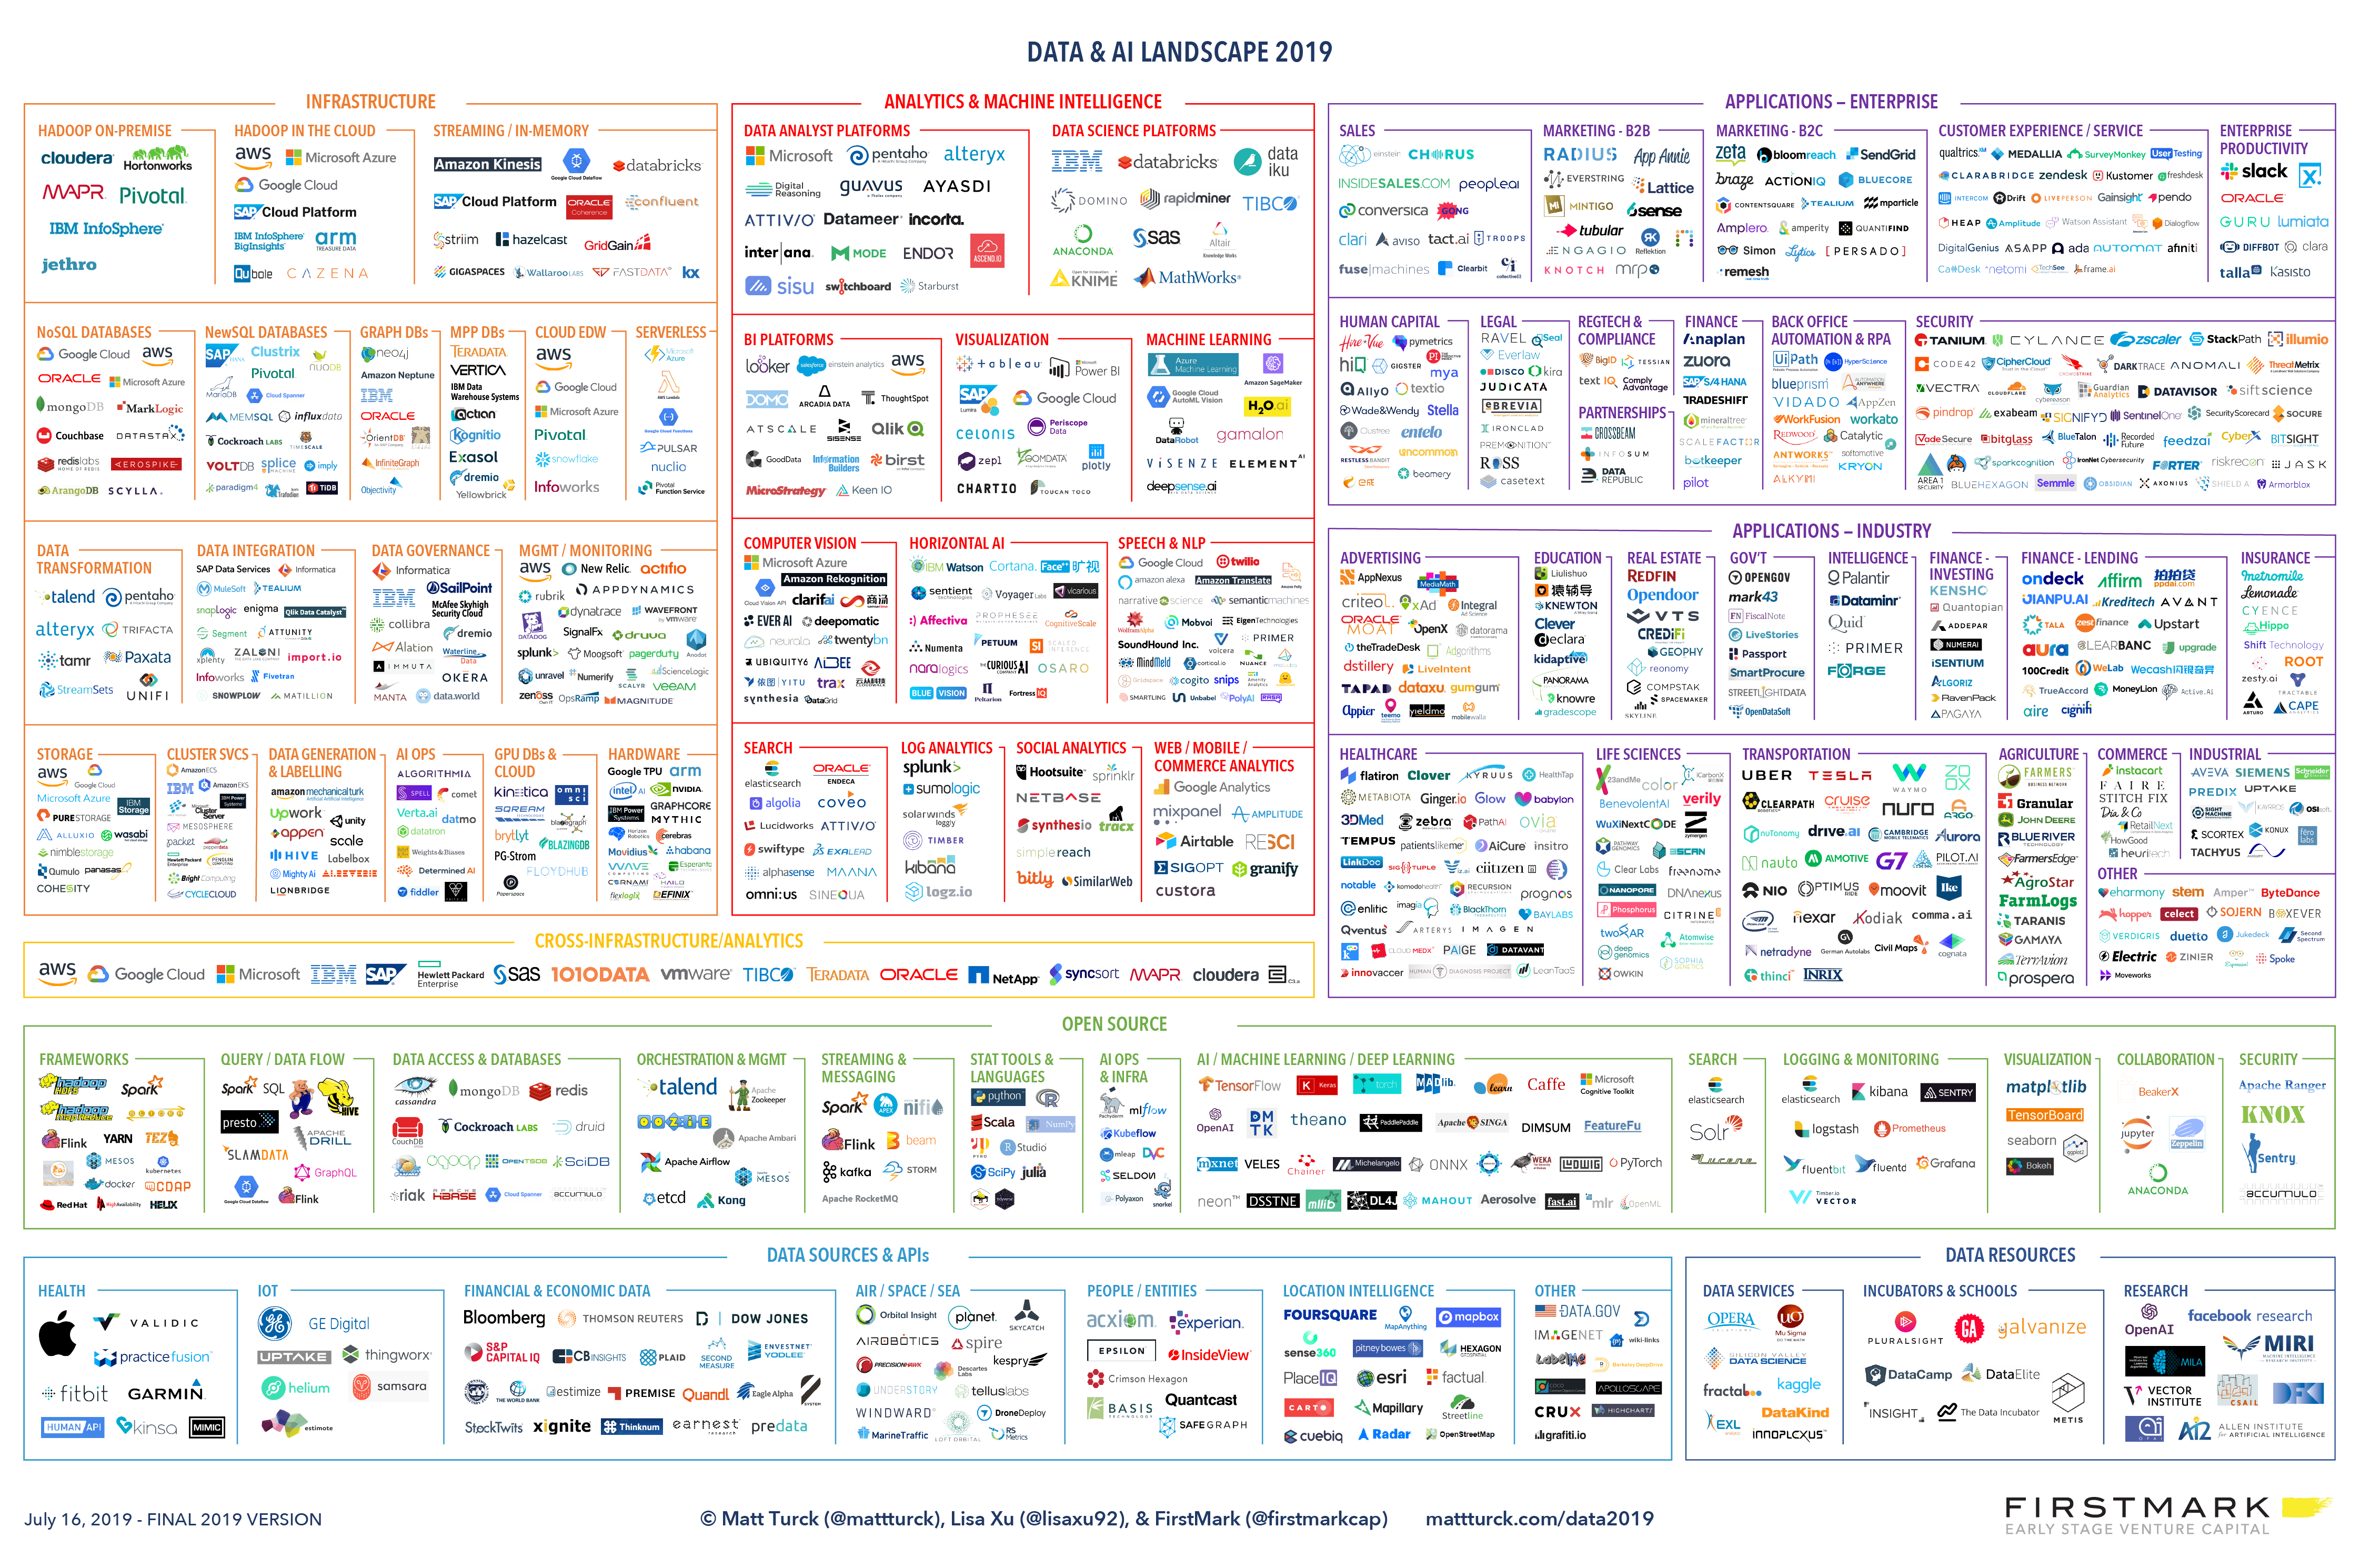
\includepdf[pages=-,angle=90]{landscape.pdf}
    \end{landscape}
\KOMAoptions{paper=a4}
\recalctypearea


\chapterimage{capitulos.pdf}
\chapter{\emph{Gartner Scores}}
\label{anexo-tabelacc}

%A próxima página apresenta tabela\footnote{A tabela original do \relatorioGCC \xspace é chamada de ``\emph{Table 2: Product/Service Rating on Critical Capabilities}.''} contendo a atribuição de notas (\emph{scores}) para cada fornecedor avaliado (horizontal) para cada uma das 15 áreas de capacidade (vertical). 

A próxima página apresenta tabela elaborada a partir do \relatorioGCC contendo a atribuição de notas (\emph{scores}) para cada fornecedor avaliado (horizontal) de cada uma das 15 áreas de capacidade (vertical).

As notas variam de $1,0$ a $5,0$ e apresentam o seguinte significado:

\begin{itemize}
    \item \textbf{1 = Fraco ou ausente}: a maioria ou todos os requisitos definidos para uma capacidade não são alcançados;   
    \item \textbf{2 = Regular}: alguns requisitos não são alcançados;
    \item \textbf{3 = Bom}: atende aos requisitos;
    \item \textbf{4 = Excelente}: atende ou excede alguns requisitos;   
    \item \textbf{5 = Excelente}: excede significativamente os requisitos;
\end{itemize}

Os resultados dos casos de uso construídos no ``\autoref{cap-casos-gartner} -- \nameref{cap-casos-gartner}'' da ``\autoref{parte-estudosdecaso} -- \nameref{parte-estudosdecaso}'' são obtidos pela soma da multiplicação dos pesos definidos para cada área de capacidade e as notas atribuídas a cada fornecedor de acordo com essa tabela. 
\thispagestyle{empty}
\begin{landscape}
    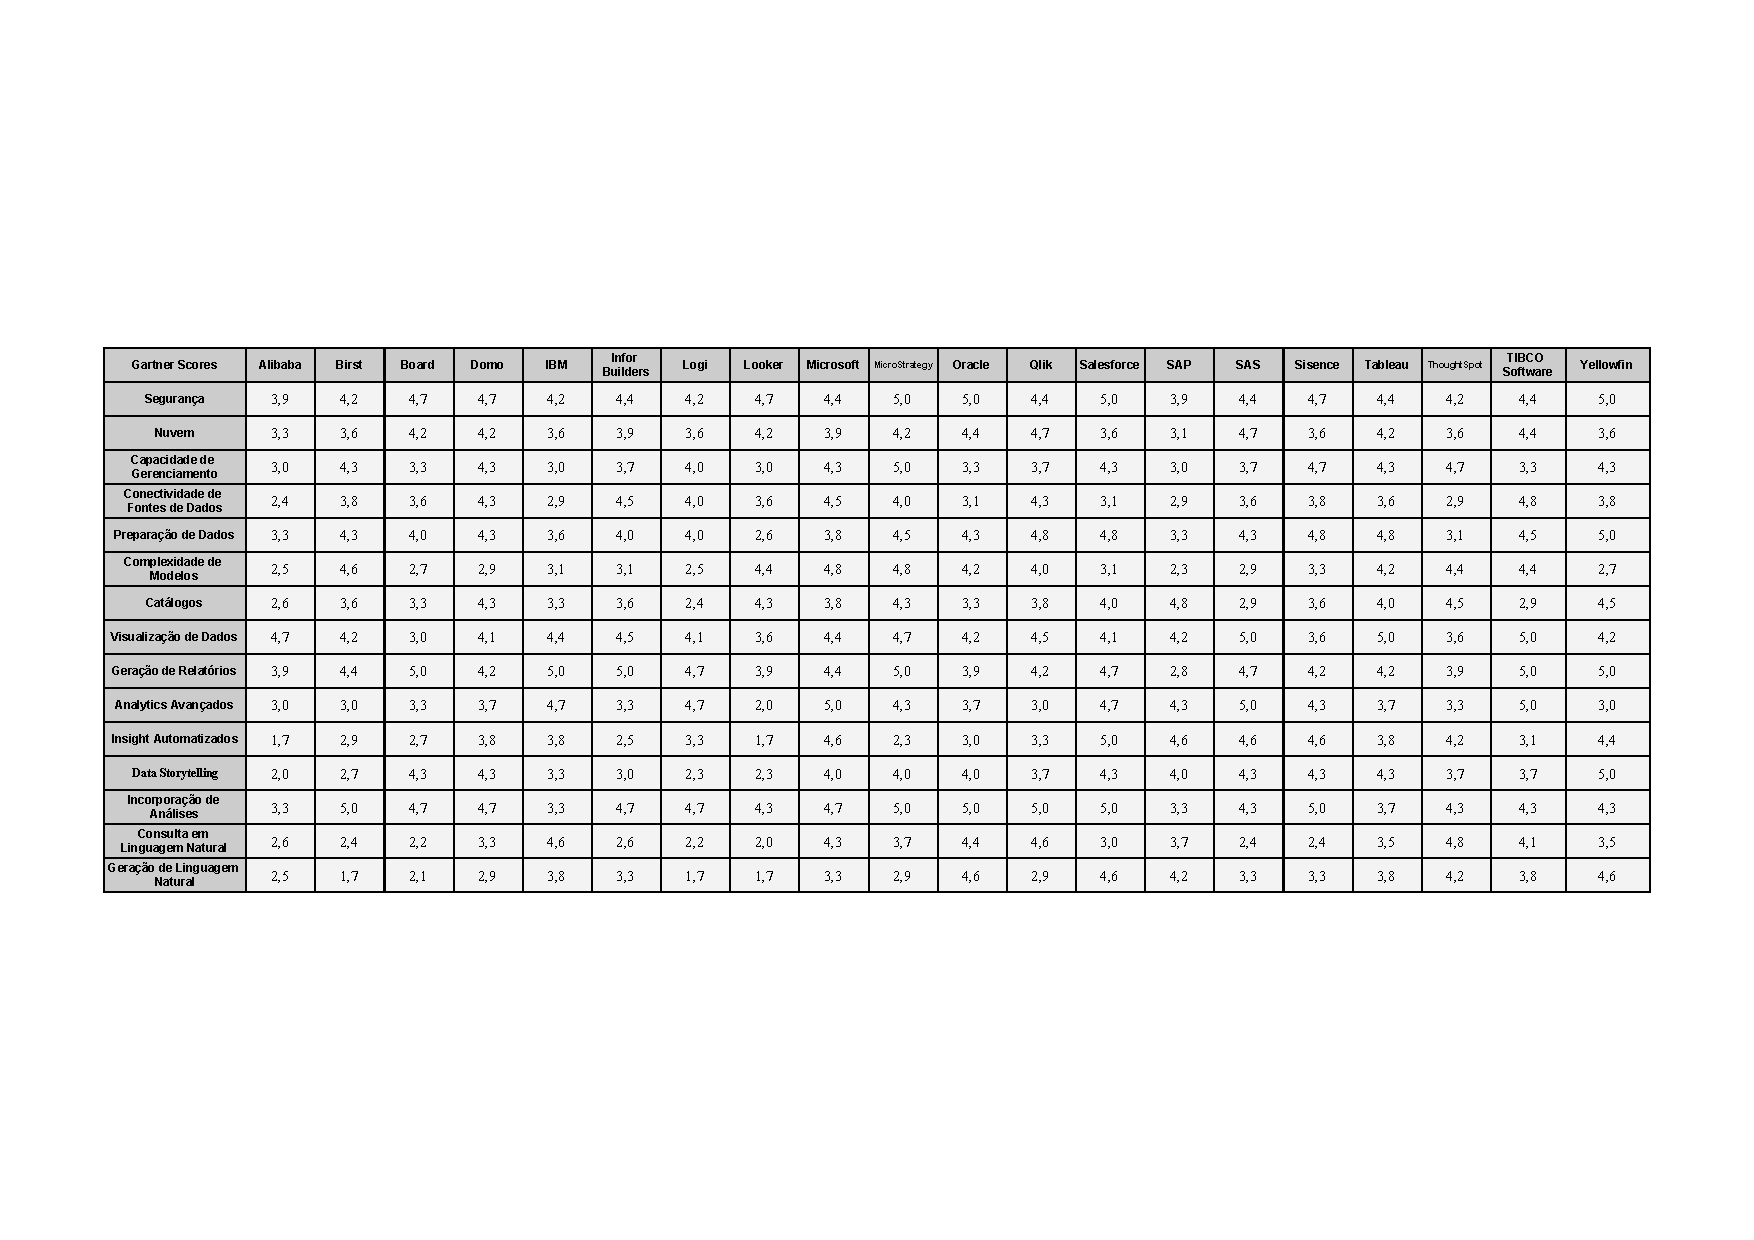
\includepdf[pages=-,angle=90]{gartner.pdf}
\end{landscape}

\chapterimage{capitulos.pdf}
\chapter{\emph{Forrester Scores}}
\label{anexo-tabelafw}

%A próxima página apresenta tabela\footnote{A tabela original do \relatorioFCM \xspace é chamada de ``\emph{FIGURE 2 Forrester WaveTM: Enterprise BI Platforms (Client-Managed) Scorecard, Q3 2019}.''} contendo a atribuição de notas (\emph{scores}) para cada fornecedor avaliado (horizontal) para cada um dos critérios (vertical).

A próxima página apresenta tabela elaborada a partir do \relatorioFCM contendo a atribuição de notas (\emph{scores}) para cada fornecedor avaliado (horizontal) de cada um dos critérios (vertical). De forma semelhante ao anexo anterior, essas notas avaliam os requisitos na escala de $1,0$ a $5,0$.

Os resultados dos casos de uso construídos no ``\autoref{cap-casos-forrester} -- \nameref{cap-casos-forrester}'' da ``\autoref{parte-estudosdecaso} -- \nameref{parte-estudosdecaso}'' são obtidos pela soma da multiplicação dos pesos definidos para cada critério e as notas atribuídas a cada fornecedor de acordo com essa tabela. 

\thispagestyle{empty}
\begin{landscape}
    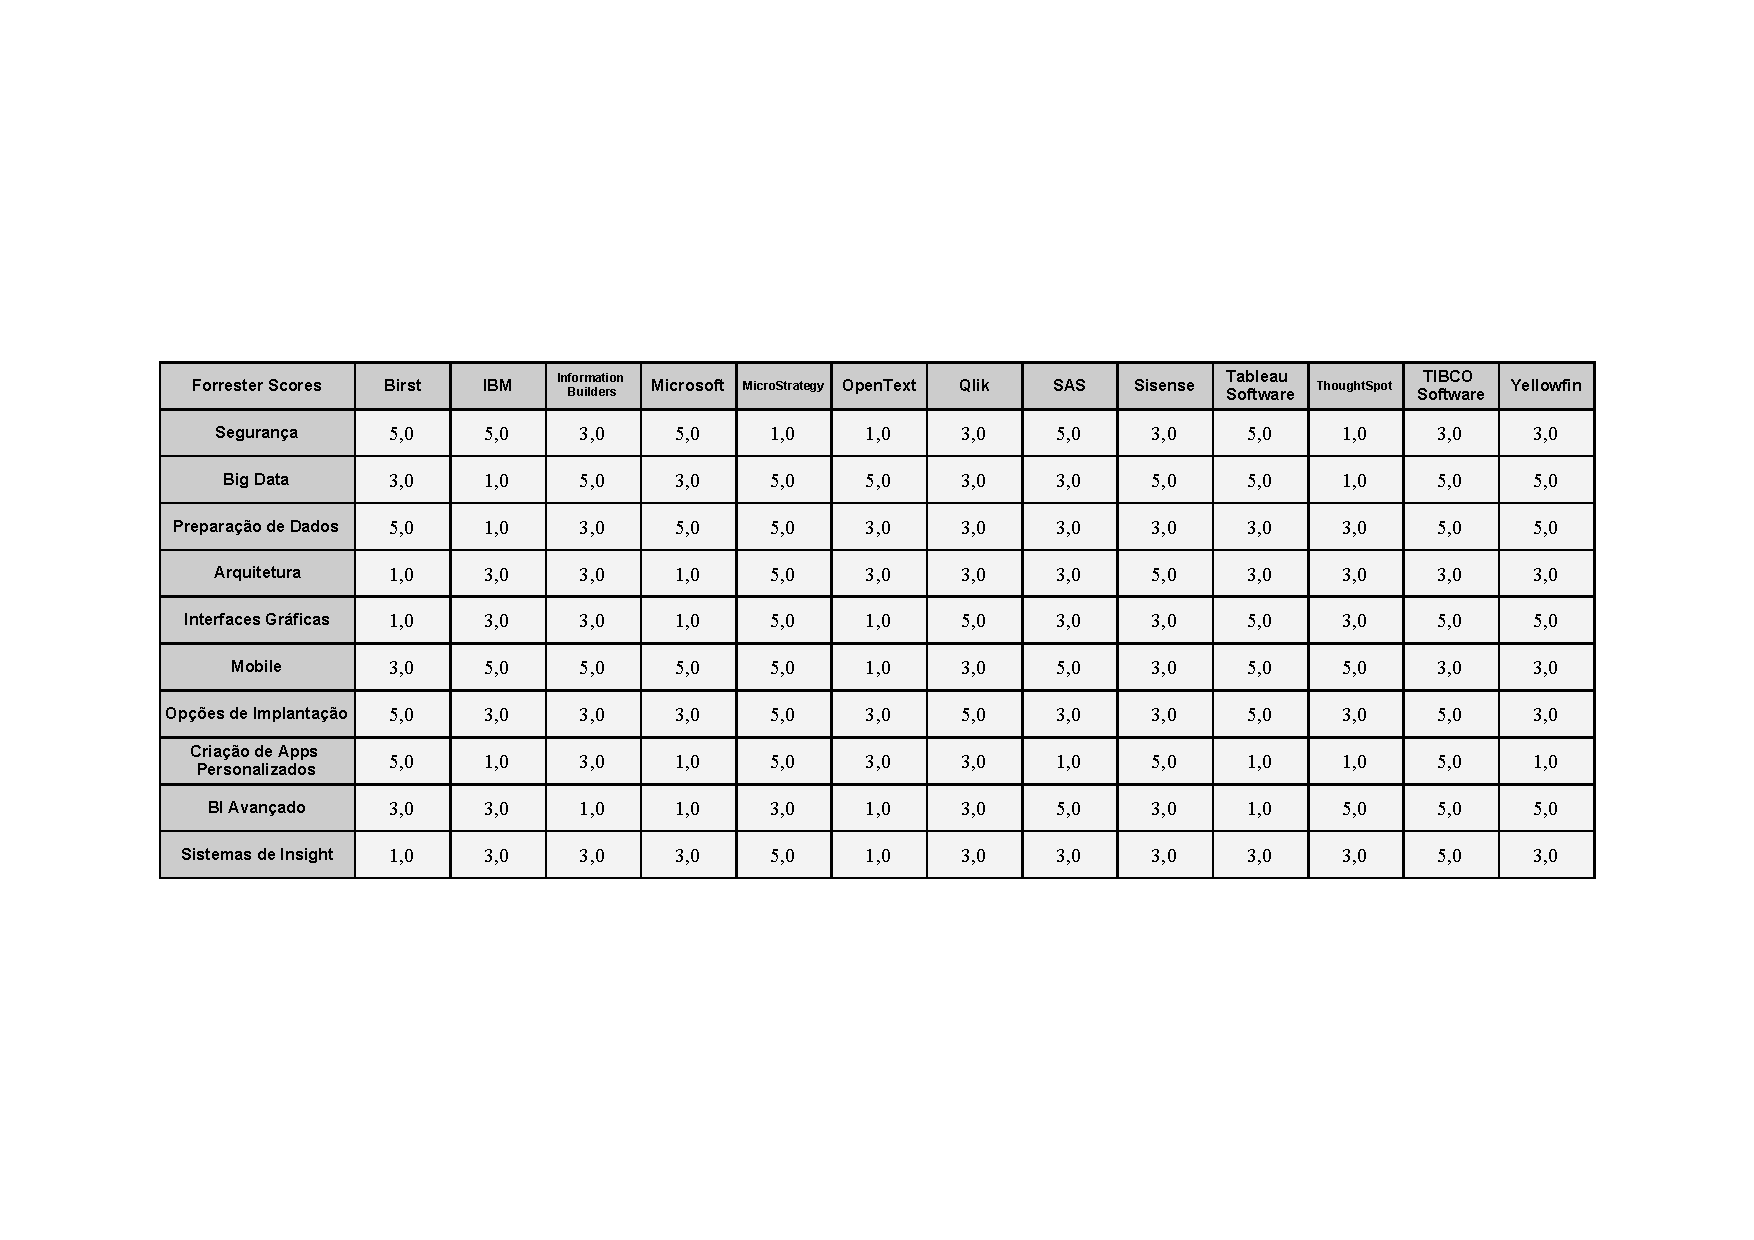
\includepdf[pages=-,angle=90]{forrester.pdf}
\end{landscape}



% ----

\end{document}
